\documentclass{article}
%DIF LATEXDIFF DIFFERENCE FILE
%DIF DEL SST_main.tex            Sun Sep 17 10:19:49 2023
%DIF ADD SST_main_polished.tex   Sun Sep 17 10:30:38 2023
\usepackage[utf8]{inputenc}
\usepackage{authblk}
\usepackage{setspace}
\usepackage[margin=1.25in]{geometry}
\usepackage{graphicx}
% \graphicspath{ {./figures/} }
\graphicspath{ {../figures/} }
\usepackage{subcaption}
\usepackage{amsmath}
\usepackage{lineno}
% \linenumbers

\usepackage{enumerate}
\DeclareMathOperator{\diag}{diag}
\usepackage{multirow}
\usepackage{booktabs}
\usepackage{footnote}
\usepackage{bm}
\usepackage[ruled,linesnumbered]{algorithm2e}
\setcounter{MaxMatrixCols}{20}
\usepackage{tikz}
\usetikzlibrary{arrows.meta, calc, fit, positioning, quotes, graphs, shapes.geometric}
\def\T{\mathrm{T}}

%DIF 26c26
%DIF < \usepackage[final]{changes}
%DIF -------
% \usepackage[final]{changes} %DIF > 
%DIF -------
% \usepackage[defaultcolor=red]{changes}
% \added{xxx}
% \deleted{xxxx}
% \replaced{a}{b}

%%%%%% Bibliography %%%%%%
% Replace "sample" in the \addbibresource line below with the name of your .bib file.
\usepackage[style=nejm, citestyle=numeric-comp, sorting=none]{biblatex}
\addbibresource{SST_main.bib}

%%%%%% Title %%%%%%
% Full titles can be a maximum of 100 characters, including spaces. 
% Title Format: Use title case, capitalizing the first letter of each word, except for certain small words, such as articles and short prepositions
%DIF 40c40
%DIF < \title{Maximum Allowable Current Determination of RBS By Using a Directed Graph Model and Greedy Algorithm}
%DIF -------
\title{Using a Directed Graph Model and Greedy Algorithm to Determine the Maximum Allowable Current in a Reconfigurable Battery System} %DIF > 
%DIF -------

%%%%%% Authors %%%%%%
% Authors should be listed in order of contribution to the paper, by first name, then middle initial (if any), followed by last name.
% Authors should be listed in the order in which they will appear in the published version if the manuscript is accepted. 
% Use an asterisk (*) to identify the corresponding author, and be sure to include that person’s e-mail address. Use symbols (in this order: †, ‡, §, ||, ¶, #, ††, ‡‡, etc.) for author notes, such as present addresses, “These authors contributed equally to this work” notations, and similar information.
% You can include group authors, but please include a list of the actual authors (the group members) in the Supplementary Materials.
\author[1]{30577}
\author[1$\dag$]{Binghui Xu}
\author[1$\dag$]{Guangbin Hua}
\author[1*]{Cheng Qian}
\author[1,2]{Quan Xia}
\author[1]{Bo Sun}
\author[1]{Yi Ren}
\author[1]{Zili Wang}

%%%%%% Affiliations %%%%%%
\affil[1]{School of Reliability and Systems Engineering, Beihang University, Beijing, 100191, China}
\affil[2]{School of Aeronautic Science and Engineering at Beihang University, Beijing, China}
\affil[*]{Address correspondence to: cqian@buaa.edu.cn}
\affil[$\dag$]{These authors contributed equally to this work.}

%%%%%% Date %%%%%%
% Date is optional
\date{}

%%%%%% Spacing %%%%%%
% Use paragraph spacing of 1.5 or 2 (for double spacing, use command \doublespacing)
\onehalfspacing
%DIF PREAMBLE EXTENSION ADDED BY LATEXDIFF
%DIF UNDERLINE PREAMBLE %DIF PREAMBLE
\RequirePackage[normalem]{ulem} %DIF PREAMBLE
\RequirePackage{color}\definecolor{RED}{rgb}{1,0,0}\definecolor{BLUE}{rgb}{0,0,1} %DIF PREAMBLE
\providecommand{\DIFadd}[1]{{\protect\color{blue}\uwave{#1}}} %DIF PREAMBLE
\providecommand{\DIFdel}[1]{{\protect\color{red}\sout{#1}}}                      %DIF PREAMBLE
%DIF SAFE PREAMBLE %DIF PREAMBLE
\providecommand{\DIFaddbegin}{} %DIF PREAMBLE
\providecommand{\DIFaddend}{} %DIF PREAMBLE
\providecommand{\DIFdelbegin}{} %DIF PREAMBLE
\providecommand{\DIFdelend}{} %DIF PREAMBLE
\providecommand{\DIFmodbegin}{} %DIF PREAMBLE
\providecommand{\DIFmodend}{} %DIF PREAMBLE
%DIF FLOATSAFE PREAMBLE %DIF PREAMBLE
\providecommand{\DIFaddFL}[1]{\DIFadd{#1}} %DIF PREAMBLE
\providecommand{\DIFdelFL}[1]{\DIFdel{#1}} %DIF PREAMBLE
\providecommand{\DIFaddbeginFL}{} %DIF PREAMBLE
\providecommand{\DIFaddendFL}{} %DIF PREAMBLE
\providecommand{\DIFdelbeginFL}{} %DIF PREAMBLE
\providecommand{\DIFdelendFL}{} %DIF PREAMBLE
\newcommand{\DIFscaledelfig}{0.5}
%DIF HIGHLIGHTGRAPHICS PREAMBLE %DIF PREAMBLE
\RequirePackage{settobox} %DIF PREAMBLE
\RequirePackage{letltxmacro} %DIF PREAMBLE
\newsavebox{\DIFdelgraphicsbox} %DIF PREAMBLE
\newlength{\DIFdelgraphicswidth} %DIF PREAMBLE
\newlength{\DIFdelgraphicsheight} %DIF PREAMBLE
% store original definition of \includegraphics %DIF PREAMBLE
\LetLtxMacro{\DIFOincludegraphics}{\includegraphics} %DIF PREAMBLE
\newcommand{\DIFaddincludegraphics}[2][]{{\color{blue}\fbox{\DIFOincludegraphics[#1]{#2}}}} %DIF PREAMBLE
\newcommand{\DIFdelincludegraphics}[2][]{% %DIF PREAMBLE
\sbox{\DIFdelgraphicsbox}{\DIFOincludegraphics[#1]{#2}}% %DIF PREAMBLE
\settoboxwidth{\DIFdelgraphicswidth}{\DIFdelgraphicsbox} %DIF PREAMBLE
\settoboxtotalheight{\DIFdelgraphicsheight}{\DIFdelgraphicsbox} %DIF PREAMBLE
\scalebox{\DIFscaledelfig}{% %DIF PREAMBLE
\parbox[b]{\DIFdelgraphicswidth}{\usebox{\DIFdelgraphicsbox}\\[-\baselineskip] \rule{\DIFdelgraphicswidth}{0em}}\llap{\resizebox{\DIFdelgraphicswidth}{\DIFdelgraphicsheight}{% %DIF PREAMBLE
\setlength{\unitlength}{\DIFdelgraphicswidth}% %DIF PREAMBLE
\begin{picture}(1,1)% %DIF PREAMBLE
\thicklines\linethickness{2pt} %DIF PREAMBLE
{\color[rgb]{1,0,0}\put(0,0){\framebox(1,1){}}}% %DIF PREAMBLE
{\color[rgb]{1,0,0}\put(0,0){\line( 1,1){1}}}% %DIF PREAMBLE
{\color[rgb]{1,0,0}\put(0,1){\line(1,-1){1}}}% %DIF PREAMBLE
\end{picture}% %DIF PREAMBLE
}\hspace*{3pt}}} %DIF PREAMBLE
} %DIF PREAMBLE
\LetLtxMacro{\DIFOaddbegin}{\DIFaddbegin} %DIF PREAMBLE
\LetLtxMacro{\DIFOaddend}{\DIFaddend} %DIF PREAMBLE
\LetLtxMacro{\DIFOdelbegin}{\DIFdelbegin} %DIF PREAMBLE
\LetLtxMacro{\DIFOdelend}{\DIFdelend} %DIF PREAMBLE
\DeclareRobustCommand{\DIFaddbegin}{\DIFOaddbegin \let\includegraphics\DIFaddincludegraphics} %DIF PREAMBLE
\DeclareRobustCommand{\DIFaddend}{\DIFOaddend \let\includegraphics\DIFOincludegraphics} %DIF PREAMBLE
\DeclareRobustCommand{\DIFdelbegin}{\DIFOdelbegin \let\includegraphics\DIFdelincludegraphics} %DIF PREAMBLE
\DeclareRobustCommand{\DIFdelend}{\DIFOaddend \let\includegraphics\DIFOincludegraphics} %DIF PREAMBLE
\LetLtxMacro{\DIFOaddbeginFL}{\DIFaddbeginFL} %DIF PREAMBLE
\LetLtxMacro{\DIFOaddendFL}{\DIFaddendFL} %DIF PREAMBLE
\LetLtxMacro{\DIFOdelbeginFL}{\DIFdelbeginFL} %DIF PREAMBLE
\LetLtxMacro{\DIFOdelendFL}{\DIFdelendFL} %DIF PREAMBLE
\DeclareRobustCommand{\DIFaddbeginFL}{\DIFOaddbeginFL \let\includegraphics\DIFaddincludegraphics} %DIF PREAMBLE
\DeclareRobustCommand{\DIFaddendFL}{\DIFOaddendFL \let\includegraphics\DIFOincludegraphics} %DIF PREAMBLE
\DeclareRobustCommand{\DIFdelbeginFL}{\DIFOdelbeginFL \let\includegraphics\DIFdelincludegraphics} %DIF PREAMBLE
\DeclareRobustCommand{\DIFdelendFL}{\DIFOaddendFL \let\includegraphics\DIFOincludegraphics} %DIF PREAMBLE
%DIF COLORLISTINGS PREAMBLE %DIF PREAMBLE
\RequirePackage{listings} %DIF PREAMBLE
\RequirePackage{color} %DIF PREAMBLE
\lstdefinelanguage{DIFcode}{ %DIF PREAMBLE
%DIF DIFCODE_UNDERLINE %DIF PREAMBLE
  moredelim=[il][\color{red}\sout]{\%DIF\ <\ }, %DIF PREAMBLE
  moredelim=[il][\color{blue}\uwave]{\%DIF\ >\ } %DIF PREAMBLE
} %DIF PREAMBLE
\lstdefinestyle{DIFverbatimstyle}{ %DIF PREAMBLE
	language=DIFcode, %DIF PREAMBLE
	basicstyle=\ttfamily, %DIF PREAMBLE
	columns=fullflexible, %DIF PREAMBLE
	keepspaces=true %DIF PREAMBLE
} %DIF PREAMBLE
\lstnewenvironment{DIFverbatim}{\lstset{style=DIFverbatimstyle}}{} %DIF PREAMBLE
\lstnewenvironment{DIFverbatim*}{\lstset{style=DIFverbatimstyle,showspaces=true}}{} %DIF PREAMBLE
%DIF END PREAMBLE EXTENSION ADDED BY LATEXDIFF

\begin{document}

\maketitle

%%%%%% Abstract %%%%%%
\begin{abstract}
Reconfigurable \DIFdelbegin \DIFdel{Battery Systems }\DIFdelend \DIFaddbegin \DIFadd{battery systems }\DIFaddend (RBSs) present a promising alternative to traditional battery systems due to their flexible and dynamically changeable topological structure \DIFdelbegin \DIFdel{subjected to }\DIFdelend \DIFaddbegin \DIFadd{that can be adapted to different }\DIFaddend battery charging and discharging strategies.
During \DIFdelbegin \DIFdel{the operation of the RBS , the Maximum Allowable Current }\DIFdelend \DIFaddbegin \DIFadd{RBS operation, the maximum allowable current }\DIFaddend (MAC) of \DIFaddbegin \DIFadd{the }\DIFaddend system that ensures \DIFaddbegin \DIFadd{that }\DIFaddend each battery's current remains within a safe range \DIFdelbegin \DIFdel{, }\DIFdelend is a critical indicator to guide the system's \DIFdelbegin \DIFdel{reconfiguring control}\DIFdelend \DIFaddbegin \DIFadd{reconfiguration}\DIFaddend , ensuring its safety and reliability. 
\DIFdelbegin \DIFdel{In this paper , we firstly propose a calculation method for }\DIFdelend \DIFaddbegin \DIFadd{This paper proposes a method to calculate }\DIFaddend the MAC of arbitrary \DIFdelbegin \DIFdel{RBS }\DIFdelend \DIFaddbegin \DIFadd{RBSs }\DIFaddend using a greedy algorithm in conjunction with a directed graph model of the RBS.
\DIFdelbegin %DIFDELCMD < \added{
%DIFDELCMD < By introducing the shortest path of the battery, the greedy algorithm transforms the enumeration of switch states in the brute force algorithm into the combination of the shortest paths, which greatly increases the efficiency of the determination of the MAC.
%DIFDELCMD < The directed graph model, based on the equivalent circuit, provides a specific method for calculating the MAC of a given structure.
%DIFDELCMD < This method has been validated on two published 4-battery-RBSs and one with more complex structure.
%DIFDELCMD < It obtaining the same results as the brute force algorithm method, while achieves significantly improved computational efficiency ($N_s 2^{N_s - N_b} \log N_b$ times faster than the brute force algorithm for a RBS with $N_b$ batteries and $N_s$ switches, theoretically).
%DIFDELCMD < The main advantage of this method is its ability to calculate the MAC of RBSs with arbitrary structures, even in the scenarios with random isolated batteries.
%DIFDELCMD < }
%DIFDELCMD < \deleted{
%DIFDELCMD < In this method, a new directed graph model is developed to model the structure of RBS, and a greedy algorithm is designed to find the possible circuit that enable MAC.
%DIFDELCMD < Then, the MAC is calculated based on the circuit in-cooperate with the equivalent model of batteries and switches. 
%DIFDELCMD < The effectiveness of the proposed method is validated by a novel and complex RBS structure. 
%DIFDELCMD < The results show that this method is capable to calculated the MAC of RBSs with different structures or different battery sizes efficiently, which proves the correctness of this method and its potential in facilitating next-generation RBS designs and applications, including battery isolation.
%DIFDELCMD < }
%DIFDELCMD < %%%
\DIFdelend \DIFaddbegin \DIFadd{By introducing the shortest path of the battery, the greedy algorithm transforms the enumeration of switch states in the brute-force algorithm into the combination of the shortest paths, which greatly increases the efficiency with which the MAC is determined.
The directed graph model, based on the equivalent circuit, provides a specific method for calculating the MAC of a given structure.
The proposed method is validated on two published 4-battery-RBSs and one with a more complex structure.
The results are the same as those of the brute-force algorithm, but the proposed method significantly improves the computational efficiency ($N_s 2^{N_s - N_b} \log_{10} N_b$ times faster than the brute force algorithm for a RBS with $N_b$ batteries and $N_s$ switches, theoretically).
The main advantage of the proposed method is its ability to calculate the MAC of RBSs with arbitrary structures, even in scenarios with random isolated batteries.
}\DIFaddend \end{abstract}

%%%%%% Main Text %%%%%%

\section{Introduction}

Battery \DIFdelbegin \DIFdel{Energy Storage Systems }\DIFdelend \DIFaddbegin \DIFadd{energy storage systems }\DIFaddend (BESSs) are extensively \DIFdelbegin \DIFdel{employed }\DIFdelend \DIFaddbegin \DIFadd{used }\DIFaddend in various applications, such as wind power plants and space power systems, to store and release high-quality electrical energy \cite{desiqueiraControlStrategySmooth2021,yangBatteryEnergyStorage2018,choCommercialResearchBattery2015,zhangDevelopmentProspectChinese2021,schwanbeckInternationalSpaceStation2019}.
Typically, a BESS consists of numerous batteries interconnected by series-parallel circuitry to provide the required capacity storage.
However, traditional BESSs, in which the batteries are connected in a fixed topology, \DIFdelbegin \DIFdel{exhibit }\DIFdelend \DIFaddbegin \DIFadd{suffer from }\DIFaddend a significant weakness in their worst battery due to the so-called cask effect.
Moreover, if \DIFdelbegin \DIFdel{this }\DIFdelend \DIFaddbegin \DIFadd{the }\DIFaddend worst battery fails \DIFdelbegin %DIFDELCMD < \replaced{from}{during} %%%
\DIFdelend \DIFaddbegin \DIFadd{during }\DIFaddend operation, it \DIFdelbegin \DIFdel{can }\DIFdelend \DIFaddbegin \DIFadd{is highly likely to }\DIFaddend exacerbate the degradation of \DIFdelbegin \DIFdel{other batteries with a high possibility}\DIFdelend \DIFaddbegin \DIFadd{the other batteries}\DIFaddend , leading to reliability and safety issues \cite{yangUnbalancedDischargingAging2016,fengPropagationMechanismsDiagnosis2019,jeevarajanBatterySafetyQualifications2012}.
These problems have become significant technical barriers in the development of new-generation space vehicles \DIFdelbegin %DIFDELCMD < \replaced{unfortunately}{and urgently need to be addressed} %%%
\DIFdelend \DIFaddbegin \DIFadd{and need to be addressed }\DIFaddend \cite{pomboHybridPowerSystem2021}.


Reconfigurable \DIFdelbegin \DIFdel{Battery System (RBS}\DIFdelend \DIFaddbegin \DIFadd{battery systems (RBSs}\DIFaddend ), which can dynamically switch \DIFaddbegin \DIFadd{as required }\DIFaddend to different circuit \DIFdelbegin \DIFdel{topology configurations as required, is }\DIFdelend \DIFaddbegin \DIFadd{topologies, are }\DIFaddend expected to solve \DIFdelbegin \DIFdel{the above problems}\DIFdelend \DIFaddbegin \DIFadd{this problem }\DIFaddend \cite{hanNextGenerationBatteryManagement2020a}.
The \DIFdelbegin \DIFdel{ability of }\DIFdelend switching circuit helps to isolate unhealthy batteries, \DIFdelbegin %DIFDELCMD < \replaced{thereby improving}{and thereby improve} %%%
\DIFdelend \DIFaddbegin \DIFadd{thereby improving }\DIFaddend the safety and reliability of the battery system.
\DIFdelbegin %DIFDELCMD < \replaced{In order to illustrate the working principle of RBS, a typical RBS structure developed by Visairo \cite{visairoReconfigurableBatteryPack2008}(Figure \ref{fig:stru-Visairo}) is taken as an example to show the reconfiguration process.}{Figure \ref{fig:stru-Visairo} shows a typical RBS structure developed by Visairo \cite{visairoReconfigurableBatteryPack2008} for dynamically adjusting the output voltage and current.}
%DIFDELCMD < %%%
\DIFdelend \DIFaddbegin \DIFadd{To illustrate the working principle of an RBS, we consider a typical RBS structure developed by Visairo \mbox{%DIFAUXCMD
\cite{visairoReconfigurableBatteryPack2008} }\hskip0pt%DIFAUXCMD
(Fig. \ref{fig:stru-Visairo}), which is taken as an example to show the reconfiguration process.
}\DIFaddend In this structure, the batteries can be connected not only in series when the switches $S_1$, $S_5$, $S_6$, $S_7$, $S_8$, $S_9$, and $S_{13}$ are closed (\DIFdelbegin \DIFdel{Figure \ref{fig:stru-Visairo-serial}) , }\DIFdelend \DIFaddbegin \DIFadd{see Fig. \ref{fig:stru-Visairo-serial}) }\DIFaddend but also in parallel when $S_1$, $S_2$, $S_3$, $S_4$, $S_5$, $S_9$, $S_{10}$, $S_{11}$, $S_{12}$, and $S_{13}$ are closed (\DIFdelbegin \DIFdel{Figure }\DIFdelend \DIFaddbegin \DIFadd{Fig. }\DIFaddend \ref{fig:stru-Visairo-parallel}).
Furthermore, when an unhealthy battery, for instance\DIFaddbegin \DIFadd{, }\DIFaddend the orange one $B_3$ in \DIFdelbegin \DIFdel{Figure }\DIFdelend \DIFaddbegin \DIFadd{Fig. }\DIFaddend \ref{fig:stru-Visairo-isolate}, appears in the RBS, it can be isolated by opening its two adjacent switches (i.e.\DIFaddbegin \DIFadd{, }\DIFaddend $S_4$ and $S_{11}$), ensuring \DIFdelbegin \DIFdel{the system still remains }\DIFdelend \DIFaddbegin \DIFadd{that the system remains in }\DIFaddend a reliable working mode.

\begin{figure}[htbp]
    \centering
    \begin{subfigure}[b]{0.45\textwidth}
        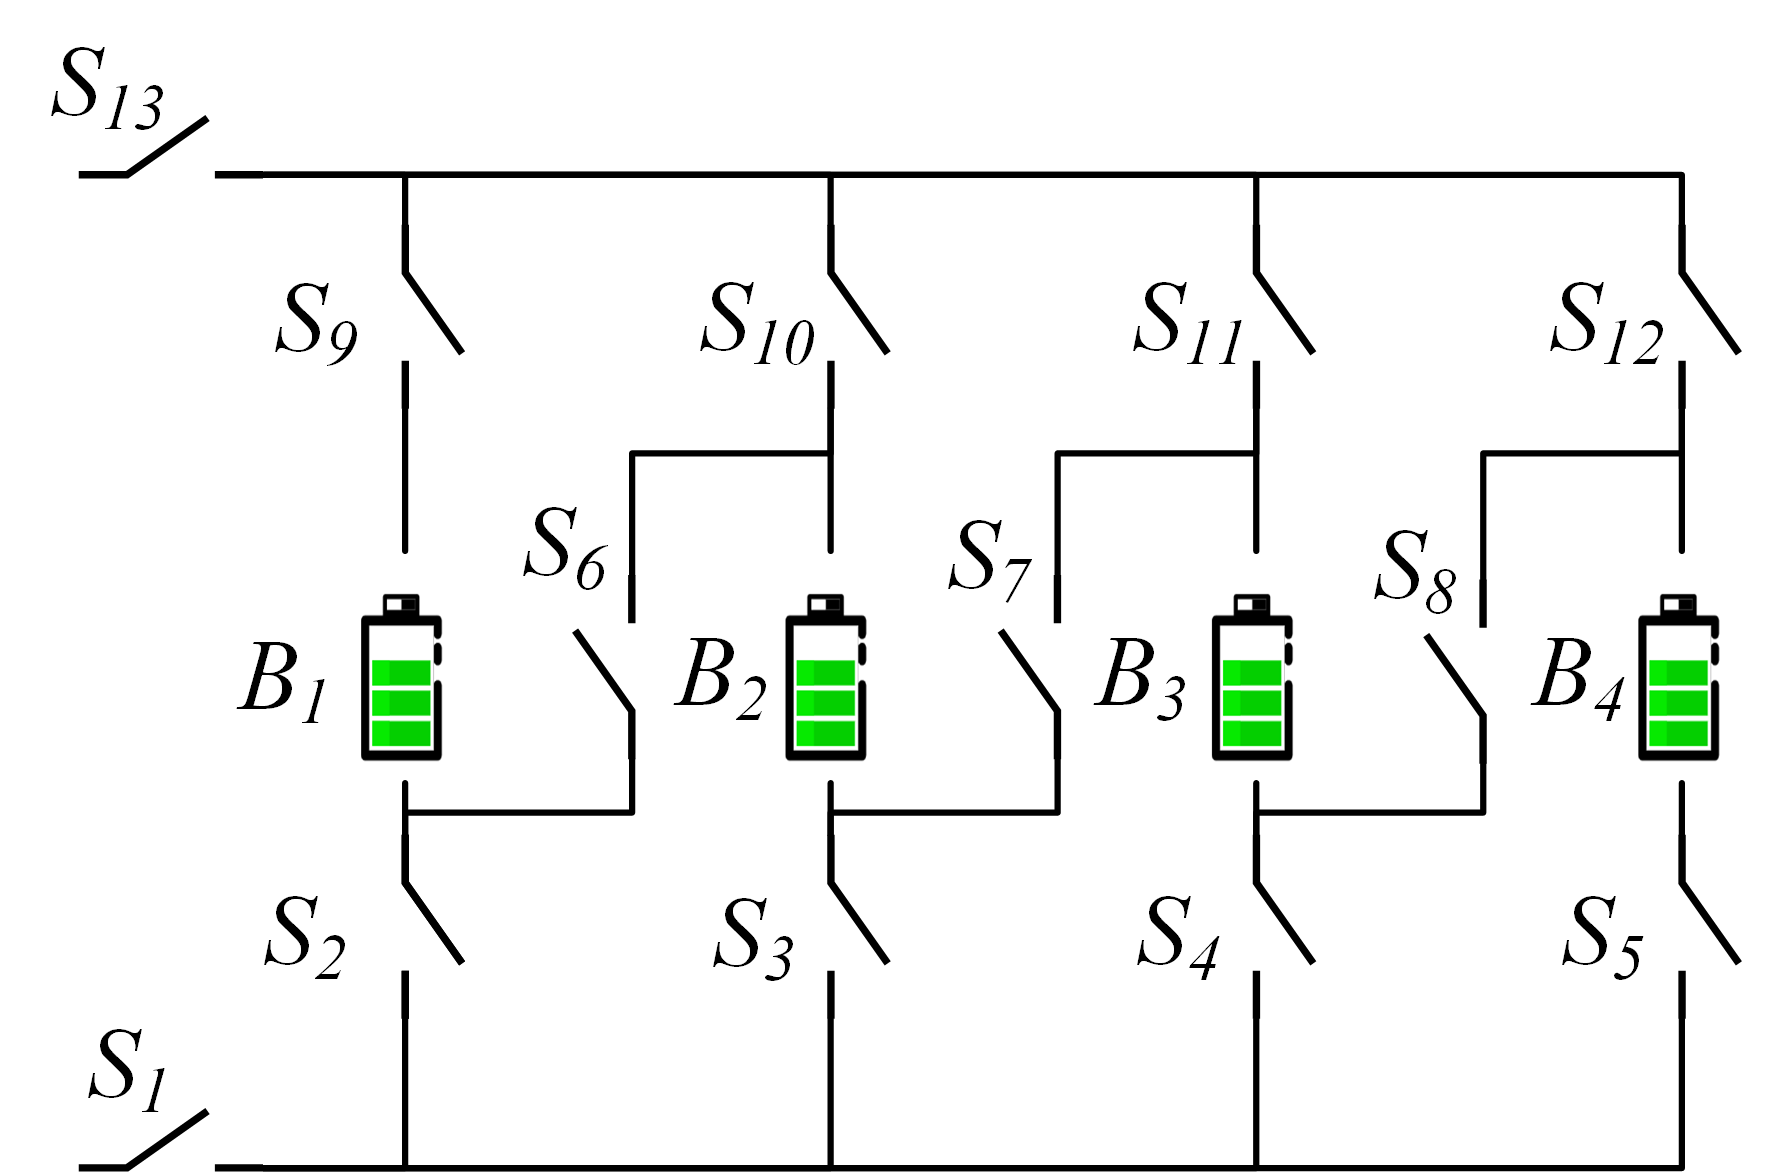
\includegraphics[width=\textwidth]{stru-V-origin.png}
        \caption{}
        \label{fig:stru-Visairo}
    \end{subfigure}
    \hspace{0.05\textwidth}
    \begin{subfigure}[b]{0.45\textwidth}
        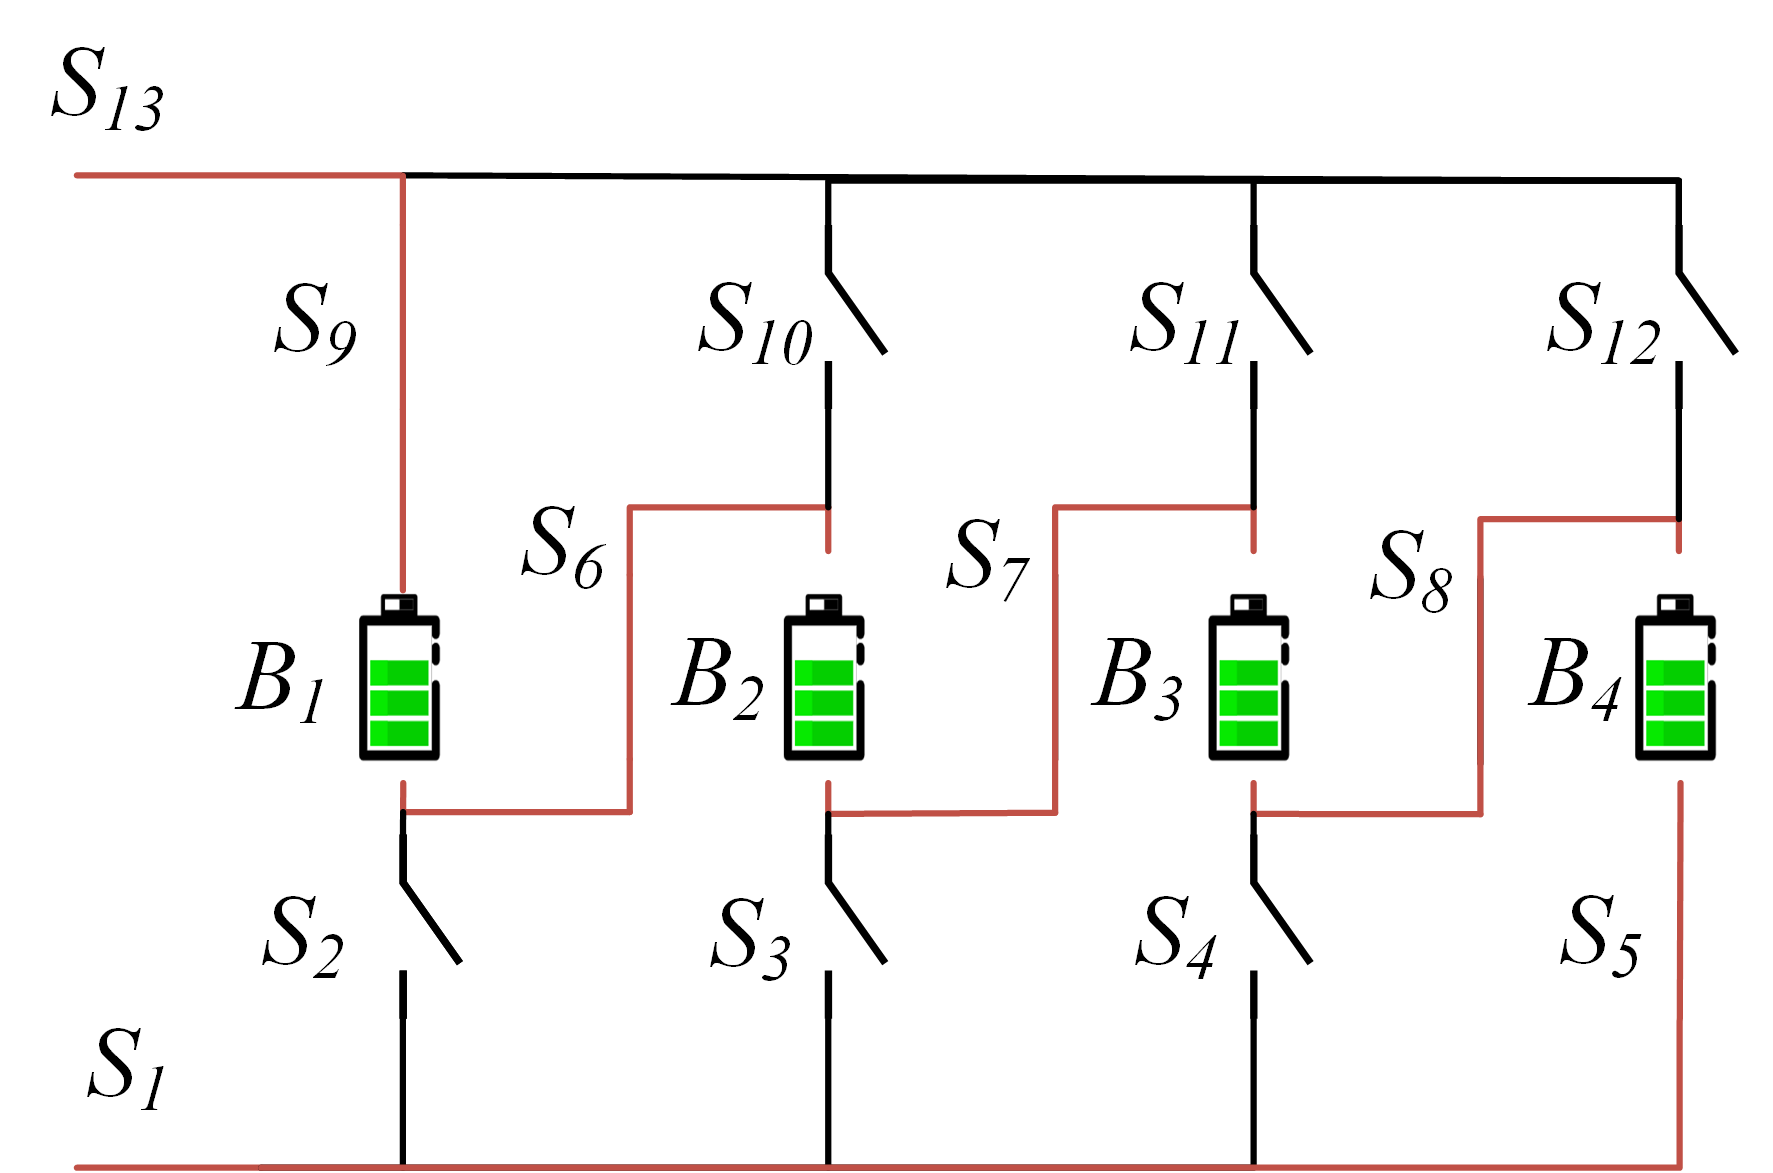
\includegraphics[width=\textwidth]{stru-V-serial.png}
        \caption{}
        \label{fig:stru-Visairo-serial}
    \end{subfigure}
    \\
    \begin{subfigure}[b]{0.45\textwidth}
        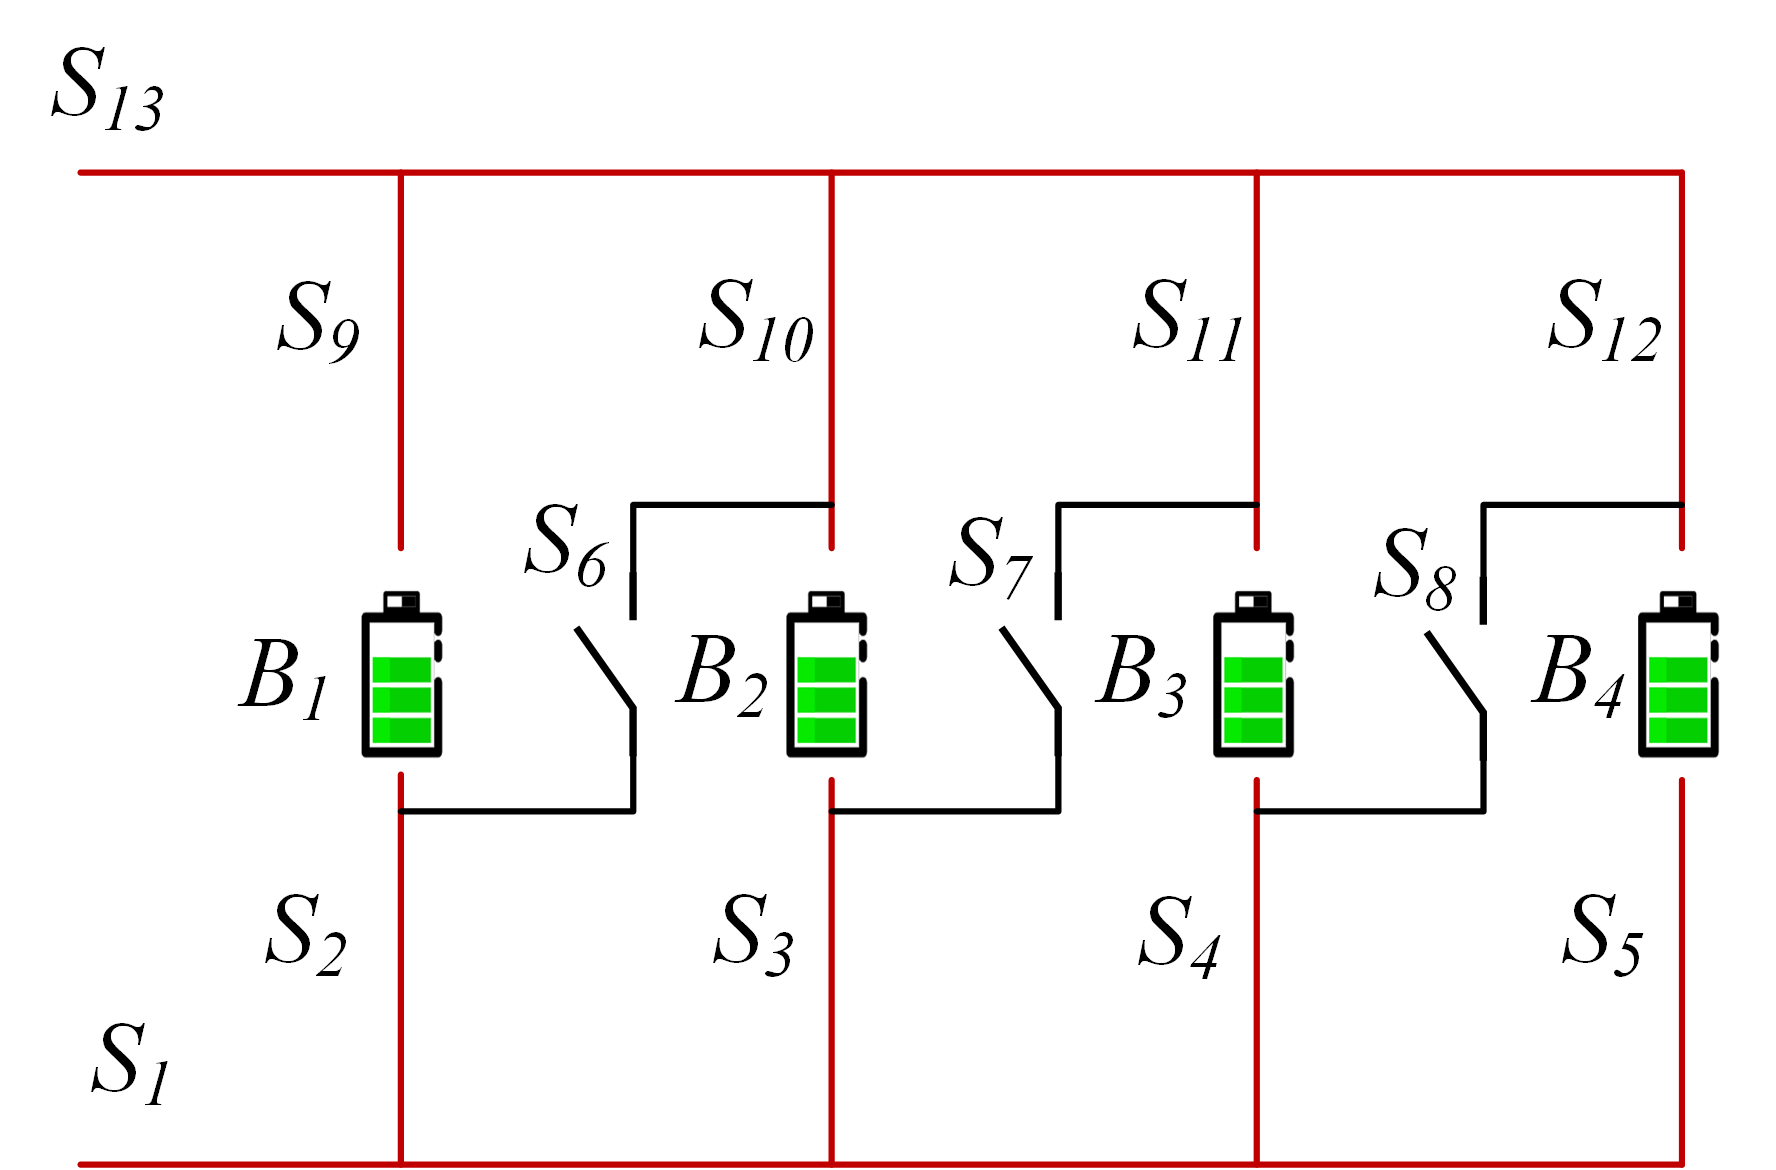
\includegraphics[width=\textwidth]{stru-V-parallel.png}
        \caption{}
        \label{fig:stru-Visairo-parallel}
    \end{subfigure}
    \hspace{0.05\textwidth}
    \begin{subfigure}[b]{0.45\textwidth}
        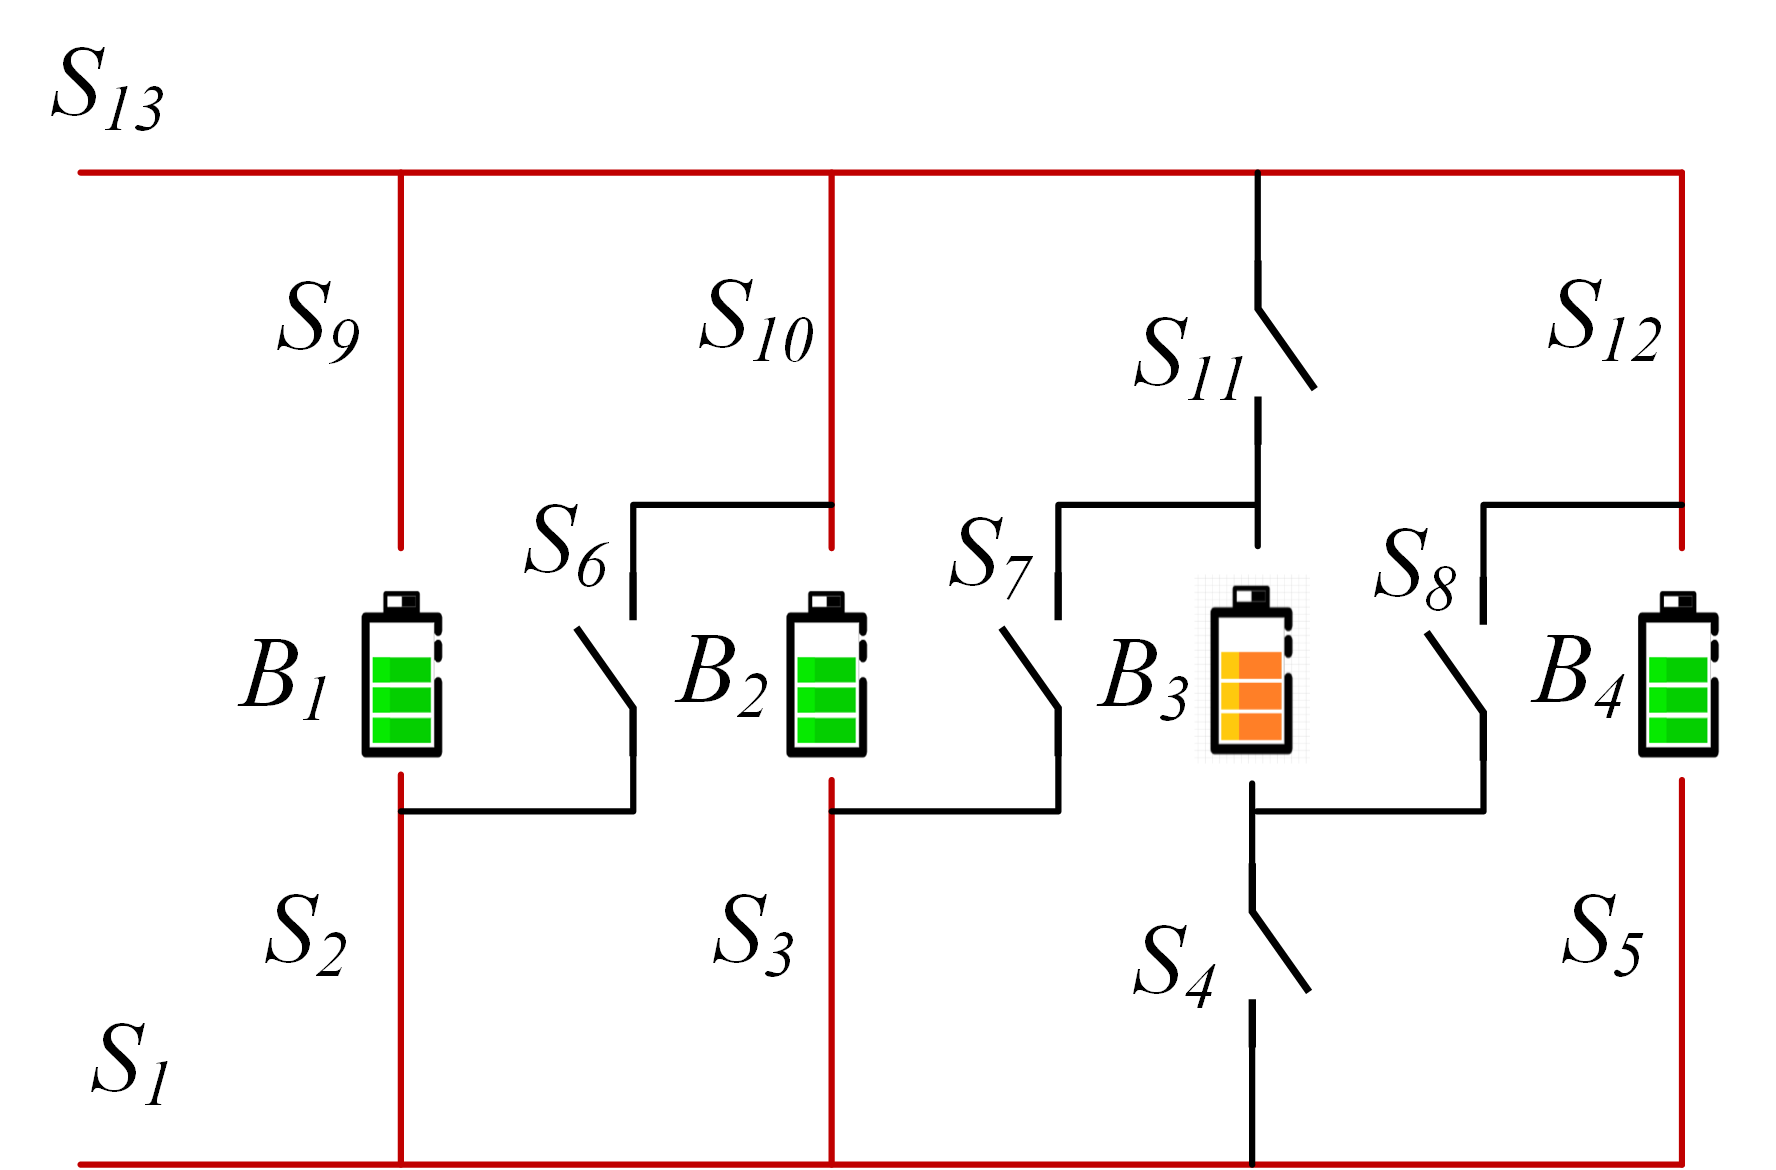
\includegraphics[width=\textwidth]{stru-V-isolate.png}
        \caption{}
        \label{fig:stru-Visairo-isolate}
    \end{subfigure}
    \caption{
        (a) The RBS structure proposed by Visairo\cite{visairoReconfigurableBatteryPack2008}, with
        all batteries in (b) series connection, (c) parallel connection, and
        (d) battery $B_3$ isolated.
        }
    \label{fig:arch}
\end{figure}


\DIFdelbegin %DIFDELCMD < \added{
%DIFDELCMD < Recently, various types of RBS with different flexibility and reconfigurability have been designed to meet application requirements. 
%DIFDELCMD < For example, Ci et al. \cite{ci2007novel} proposed a RBS structure that can dynamically adjust the batteries discharge rate to fully exploit the available capacity of each battery. 
%DIFDELCMD < Jan's \cite{9209774,engelhardt2021double} structures had the ability to reconfigure structures with variant batteries in series to reach the voltage requirements during electric vehicle charging, which constantly change.
%DIFDELCMD < The structure proposed by Visairo et al.\cite{visairoReconfigurableBatteryPack2008}, as shown in Figure \ref{fig:stru-Visairo}, can change the system's output voltage based on load conditions, thereby reducing the power loss of the voltage regulator during the power supply process and improving energy utilization efficiency. 
%DIFDELCMD < For the same purpose to enhance the energy efficiency of the system, Lawson et al. \cite{lawsonSoftwareConfigurableBattery2012} and He et al. \cite{he2014reconfiguration} also proposed simplified structures which has less switches than Visairo's design.
%DIFDELCMD < Kim et al. \cite{kim2009dynamic} improved the system's ability to recover from battery failures by introducing multiple ports to the structure. 
%DIFDELCMD < The complex structure between batteries and switches enables the flexibility of RBS, but also brings the challenges in design and control of system. 
%DIFDELCMD < Thus, several approaches to analyze the RBS structure and performance have been proposed in the literature to tackle these challenges.
%DIFDELCMD < For instance, 
%DIFDELCMD < Han et al.\cite{han2021analysis} derived an analytical expression for the maximum switch current during battery system reconfiguration for a specific RBS structure. 
%DIFDELCMD < This helps guide the selection of switches and provide support for the hardware design of RBS.
%DIFDELCMD < Chen et al.\cite{chenSneakCircuitTheory2021} proposed a systematic approach based on the sneak circuit theory to fundamentally avoid the short-circuit problem of reconfigurable battery systems. 
%DIFDELCMD < They thoroughly analyzes all paths between the cathode and anode of each battery in the RBS and identifies paths that only contain switches as short-circuit paths for pre-checking before system reconfiguration. 
%DIFDELCMD < }
%DIFDELCMD < %%%
\DIFdelend \DIFaddbegin \DIFadd{Recently, various types of RBSs with different flexibility and reconfigurability have been designed to meet application requirements. 
For example, Ci et al. \mbox{%DIFAUXCMD
\cite{ci2007novel} }\hskip0pt%DIFAUXCMD
proposed an RBS structure that dynamically adjusts the battery discharge rate to fully exploit the available capacity of each battery. 
Jan's \mbox{%DIFAUXCMD
\cite{9209774,engelhardt2021double} }\hskip0pt%DIFAUXCMD
structures  reconfigure structures with variant batteries in series to reach the (constantly changing) voltage requirements during electric vehicle charging.
As shown in Fig. \ref{fig:stru-Visairo}, the structure proposed by Visairo et al. \mbox{%DIFAUXCMD
\cite{visairoReconfigurableBatteryPack2008}  }\hskip0pt%DIFAUXCMD
changes the system's output voltage based on the load conditions, thereby reducing the power loss of the voltage regulator during the power supply process and improving the efficiency of energy use. 
Also, to enhance the energy efficiency of the system, Lawson et al. \mbox{%DIFAUXCMD
\cite{lawsonSoftwareConfigurableBattery2012} }\hskip0pt%DIFAUXCMD
and He et al. \mbox{%DIFAUXCMD
\cite{he2014reconfiguration}  }\hskip0pt%DIFAUXCMD
proposed simplified structures that have fewer switches than Visairo's design.
Kim et al. \mbox{%DIFAUXCMD
\cite{kim2009dynamic} }\hskip0pt%DIFAUXCMD
improved the system's ability to recover from battery failures by introducing multiple ports into the structure. 
}\DIFaddend 

\DIFdelbegin %DIFDELCMD < \added{
%DIFDELCMD < In spite of maximum switch current mentioned above, the maximum allowable current (MAC), defined as the maximum current allowed by system under the constraints of the battery cell, is another critical indictor of RBS that need to be evaluated during the design or control process of system. 
%DIFDELCMD < It helps the designers to assess whether the RBS meets the output current requirements, and contribute to the formulation of appropriate and safe management strategies for the battery management system (BMS).
%DIFDELCMD < Unfortunately, few studies on the RBS structure analysis have been conducted to determine the MAC of RBSs.
%DIFDELCMD < A intuitive and straightforward method is to enumerate all possible switch states and calculate the output current of the system under each reconfigurated structure.
%DIFDELCMD < But this method is inefficient and time-consuming, especially for RBSs with a large number of switches.
%DIFDELCMD < }
%DIFDELCMD < %%%
\DIFdelend \DIFaddbegin \DIFadd{The complex structure between batteries and switches gives RBSs flexibility but also creates challenges in the design and control of the system. 
Thus, several approaches to analyze the RBS structure and performance have been proposed to tackle these challenges.
For instance, 
Han et al. \mbox{%DIFAUXCMD
\cite{han2021analysis} }\hskip0pt%DIFAUXCMD
derived an analytical expression for the maximum switch current during battery system reconfiguration for a specific RBS structure. 
This helps guide the selection of switches and supports the design of RBS hardware.
Chen et al. \mbox{%DIFAUXCMD
\cite{chenSneakCircuitTheory2021} }\hskip0pt%DIFAUXCMD
proposed a systematic approach based on  sneak circuit theory to fundamentally avoid the short-circuit problem of RBSs: 
They thoroughly analyzed all paths between the cathode and anode of each battery in the RBS and identified paths that only contain switches as short-circuit paths for pre-checking before system reconfiguration. 
}\DIFaddend 



\DIFdelbegin %DIFDELCMD < \deleted{
%DIFDELCMD < The complex connection structure between batteries and switches in the RBS provides flexibility but also introduces challenges in design and operational control. 
%DIFDELCMD < Unlike traditional BESSs with fixed outputs, the RBS output must be dynamically adjusted by controlling switch states to meet external load requirements. 
%DIFDELCMD < This necessitates additional, time-consuming output performance analysis during design and corresponding control strategies. 
%DIFDELCMD < An incorrect switch control strategy may cause battery short-circuiting or overload, risking the entire system. 
%DIFDELCMD < The Maximum Allowable Current (MAC), an RBS performance indicator, can guide designers in addressing this issue. 
%DIFDELCMD < MAC is defined as the maximum RBS output current that ensures each battery's current remains within a safe range.
%DIFDELCMD < Therefore, it provides a benchmark for RBS output current, protecting individual batteries and identifying overall system output limits during operation. 
%DIFDELCMD < Despite its importance, no method currently exists for automatically evaluating MAC for RBSs.
%DIFDELCMD < In particular, when one or more random cells are isolated, there is still no method to determine the MAC of the remaining RBS in time to assist the system in adjusting the control strategy timely. 
%DIFDELCMD < A universal and automatical method for calculating RBS MAC is urgently needed for practical applications.
%DIFDELCMD < }
%DIFDELCMD < %%%
\DIFdelend \DIFaddbegin \DIFadd{In spite of the maximum switch current mentioned above, the maximum allowable current (MAC), defined as the maximum allowed current  under the constraints of the battery cell, is another critical indicator of RBSs that needs to be evaluated during the design or control  of the system. 
The MAC helps the designers assess whether the RBS meets the output current requirements and contributes to the formulation of appropriate and safe management strategies for the battery management system.
Unfortunately, few studies have analyzed the RBS structure to determine the RBS MAC.
An intuitive and straightforward method is to enumerate all possible switch states and calculate the output current of the system under each reconfigurated structure.
However, this method is inefficient and time-consuming, especially for RBSs with a large number of switches.
}\DIFaddend 




\DIFdelbegin %DIFDELCMD < \added{
%DIFDELCMD < To solve this issue, a new method to effectively evaluate the MAC of RBS is proposed in this paper. 
%DIFDELCMD < First, a greedy algorithm is designed to search the possible circuit topology of RBS with MAC effciently.
%DIFDELCMD < Meanwhile, an improved direct graph model, considering the voltage, internal resistance, and maximum allowable current of the battery, and the external load, is porposed to obtain the accurate current value of RBS under specific circuit topology. 
%DIFDELCMD < To the best of our knowledge, the present work is the first to develop an efficient calculation method of RBS MAC.
%DIFDELCMD < }
%DIFDELCMD < \deleted{In this study, a directed graph model and greedy algorithm are employed to determine the MAC of RBS and the corresponding control strategy, effectively calculating the MAC for RBSs with arbitrary structures, including scenarios with isolated batteries.}
%DIFDELCMD < \added{The main contributions of the paper can be summarized as follows:}
%DIFDELCMD < %%%
\DIFdelend \DIFaddbegin \DIFadd{To solve this issue, this paper proposes an efficient method to evaluate the MAC of RBSs. 
First, a greedy algorithm is designed to efficiently search the possible circuit topology of RBSs with MAC.
Moreover, the method provides an improved direct graph model that considers the voltage, the internal resistance, the MAC of the battery, and the external load. The method obtains the accurate current of the RBS under a specific circuit topology. 
The main contributions of this paper can be summarized as follows:
}\DIFaddend \begin{itemize}
  \item \DIFdelbegin %DIFDELCMD < \added{Proposing a effective method to determine the MAC of RBSs with arbitrary structures, including scenarios with isolated batteries.}
%DIFDELCMD <   %%%
\DIFdelend \DIFaddbegin \DIFadd{An efficient method is proposed to determine the MAC of RBSs with arbitrary structures, including scenarios with isolated batteries.
  }\DIFaddend \item \DIFdelbegin %DIFDELCMD < \added{Application of the greedy algorithm to solve the MAC problem, whose computational complexity is greatly reduced compared with the brute force algorithm.}
%DIFDELCMD <   %%%
\DIFdelend \DIFaddbegin \DIFadd{The greedy algorithm is applied to solve the MAC problem, the computational complexity of which is greatly reduced compared with the brute-force algorithm.
  }\DIFaddend \item \DIFdelbegin %DIFDELCMD < \added{introducing an improved directed graph model, considering the voltage, internal resistance, and maximum allowable current of the battery, and the external load, to achieve the current analysis of the RBS.}
%DIFDELCMD < %%%
\DIFdelend \DIFaddbegin \DIFadd{An improved directed graph model is introduced; it considers the voltage, the internal resistance, the MAC of the battery, and the external load to analyze the current of the RBS.
}\DIFaddend \end{itemize}


The remainder of this paper is organized as follows: 
Section II presents the framework and details of the proposed directed graph model and  \DIFdelbegin \DIFdel{the }\DIFdelend greedy algorithm. 
Section III \DIFdelbegin \DIFdel{demonstrated }\DIFdelend \DIFaddbegin \DIFadd{discusses }\DIFaddend a case study \DIFdelbegin \DIFdel{of using }\DIFdelend \DIFaddbegin \DIFadd{that uses }\DIFaddend the proposed method to determine the MAC of a novel\DIFdelbegin \DIFdel{and }\DIFdelend \DIFaddbegin \DIFadd{, }\DIFaddend complex structure. 
The calculation results\DIFdelbegin %DIFDELCMD < \added{, the algorithm's computational complexity} %%%
\DIFdelend \DIFaddbegin \DIFadd{, the algorithm's computational complexity, }\DIFaddend and scenarios such as \DIFdelbegin \DIFdel{batteries isolation also are }\DIFdelend \DIFaddbegin \DIFadd{battery isolation are also }\DIFaddend discussed. 
Finally, the concluding remarks are \DIFdelbegin \DIFdel{drawn in Section }\DIFdelend \DIFaddbegin \DIFadd{presented in Sec. }\DIFaddend IV.

\section{Methodology}

The central principle of this method is to \DIFdelbegin \DIFdel{make }\DIFdelend \DIFaddbegin \DIFadd{connect }\DIFaddend the batteries in \DIFdelbegin \DIFdel{RBS connected in parallel as much as }\DIFdelend \DIFaddbegin \DIFadd{an RBS in parallel to the extent }\DIFaddend possible, thereby maximizing the output current of the RBS.
To \DIFaddbegin \DIFadd{achieve this }\DIFaddend universally and automatically\DIFdelbegin \DIFdel{achieve this}\DIFdelend , the overall process is divided into \DIFdelbegin \DIFdel{four steps, as shown in Figure \ref{fig:main}.
Firstly}\DIFdelend \DIFaddbegin \DIFadd{the four steps shown in Fig. \ref{fig:main}.
First}\DIFaddend , a directed graph model is established for subsequent \DIFdelbegin %DIFDELCMD < \replaced{computations.}{computing,} \replaced{The model}{, which} %%%
\DIFdelend \DIFaddbegin \DIFadd{computations. The model }\DIFaddend not only contains the connected relationships between batteries and switches \DIFdelbegin \DIFdel{, }\DIFdelend but also retains the performance parameters of the batteries.
Subsequently, based on the equivalent circuit, the MAC problem is transformed into specific objective functions and constraints.
\DIFdelbegin \DIFdel{Then, the }\DIFdelend \DIFaddbegin \DIFadd{The }\DIFaddend shortest paths (\DIFdelbegin %DIFDELCMD < \replaced{$SP$}{SP}%%%
\DIFdelend \DIFaddbegin \DIFadd{$SP$}\DIFaddend s, where additional batteries and switches on the path are penalized as distance) for the batteries are \DIFdelbegin \DIFdel{obtained }\DIFdelend \DIFaddbegin \DIFadd{then obtained  by }\DIFaddend using the Dijkstra algorithm to \DIFdelbegin \DIFdel{guide }\DIFdelend \DIFaddbegin \DIFadd{connect }\DIFaddend the batteries in the RBS \DIFdelbegin \DIFdel{connect }\DIFdelend in parallel.
Finally, a greedy algorithm is \DIFdelbegin \DIFdel{employed }\DIFdelend \DIFaddbegin \DIFadd{used }\DIFaddend to organize the switches, allowing the batteries to connect via their \DIFdelbegin %DIFDELCMD < \replaced{$SP$}{SP}%%%
\DIFdelend \DIFaddbegin \DIFadd{$SP$}\DIFaddend s while satisfying the constraints, resulting in the MAC of the RBS.

\begin{figure}[htbp]
    \centering
    \begin{subfigure}[b]{0.8\textwidth}
        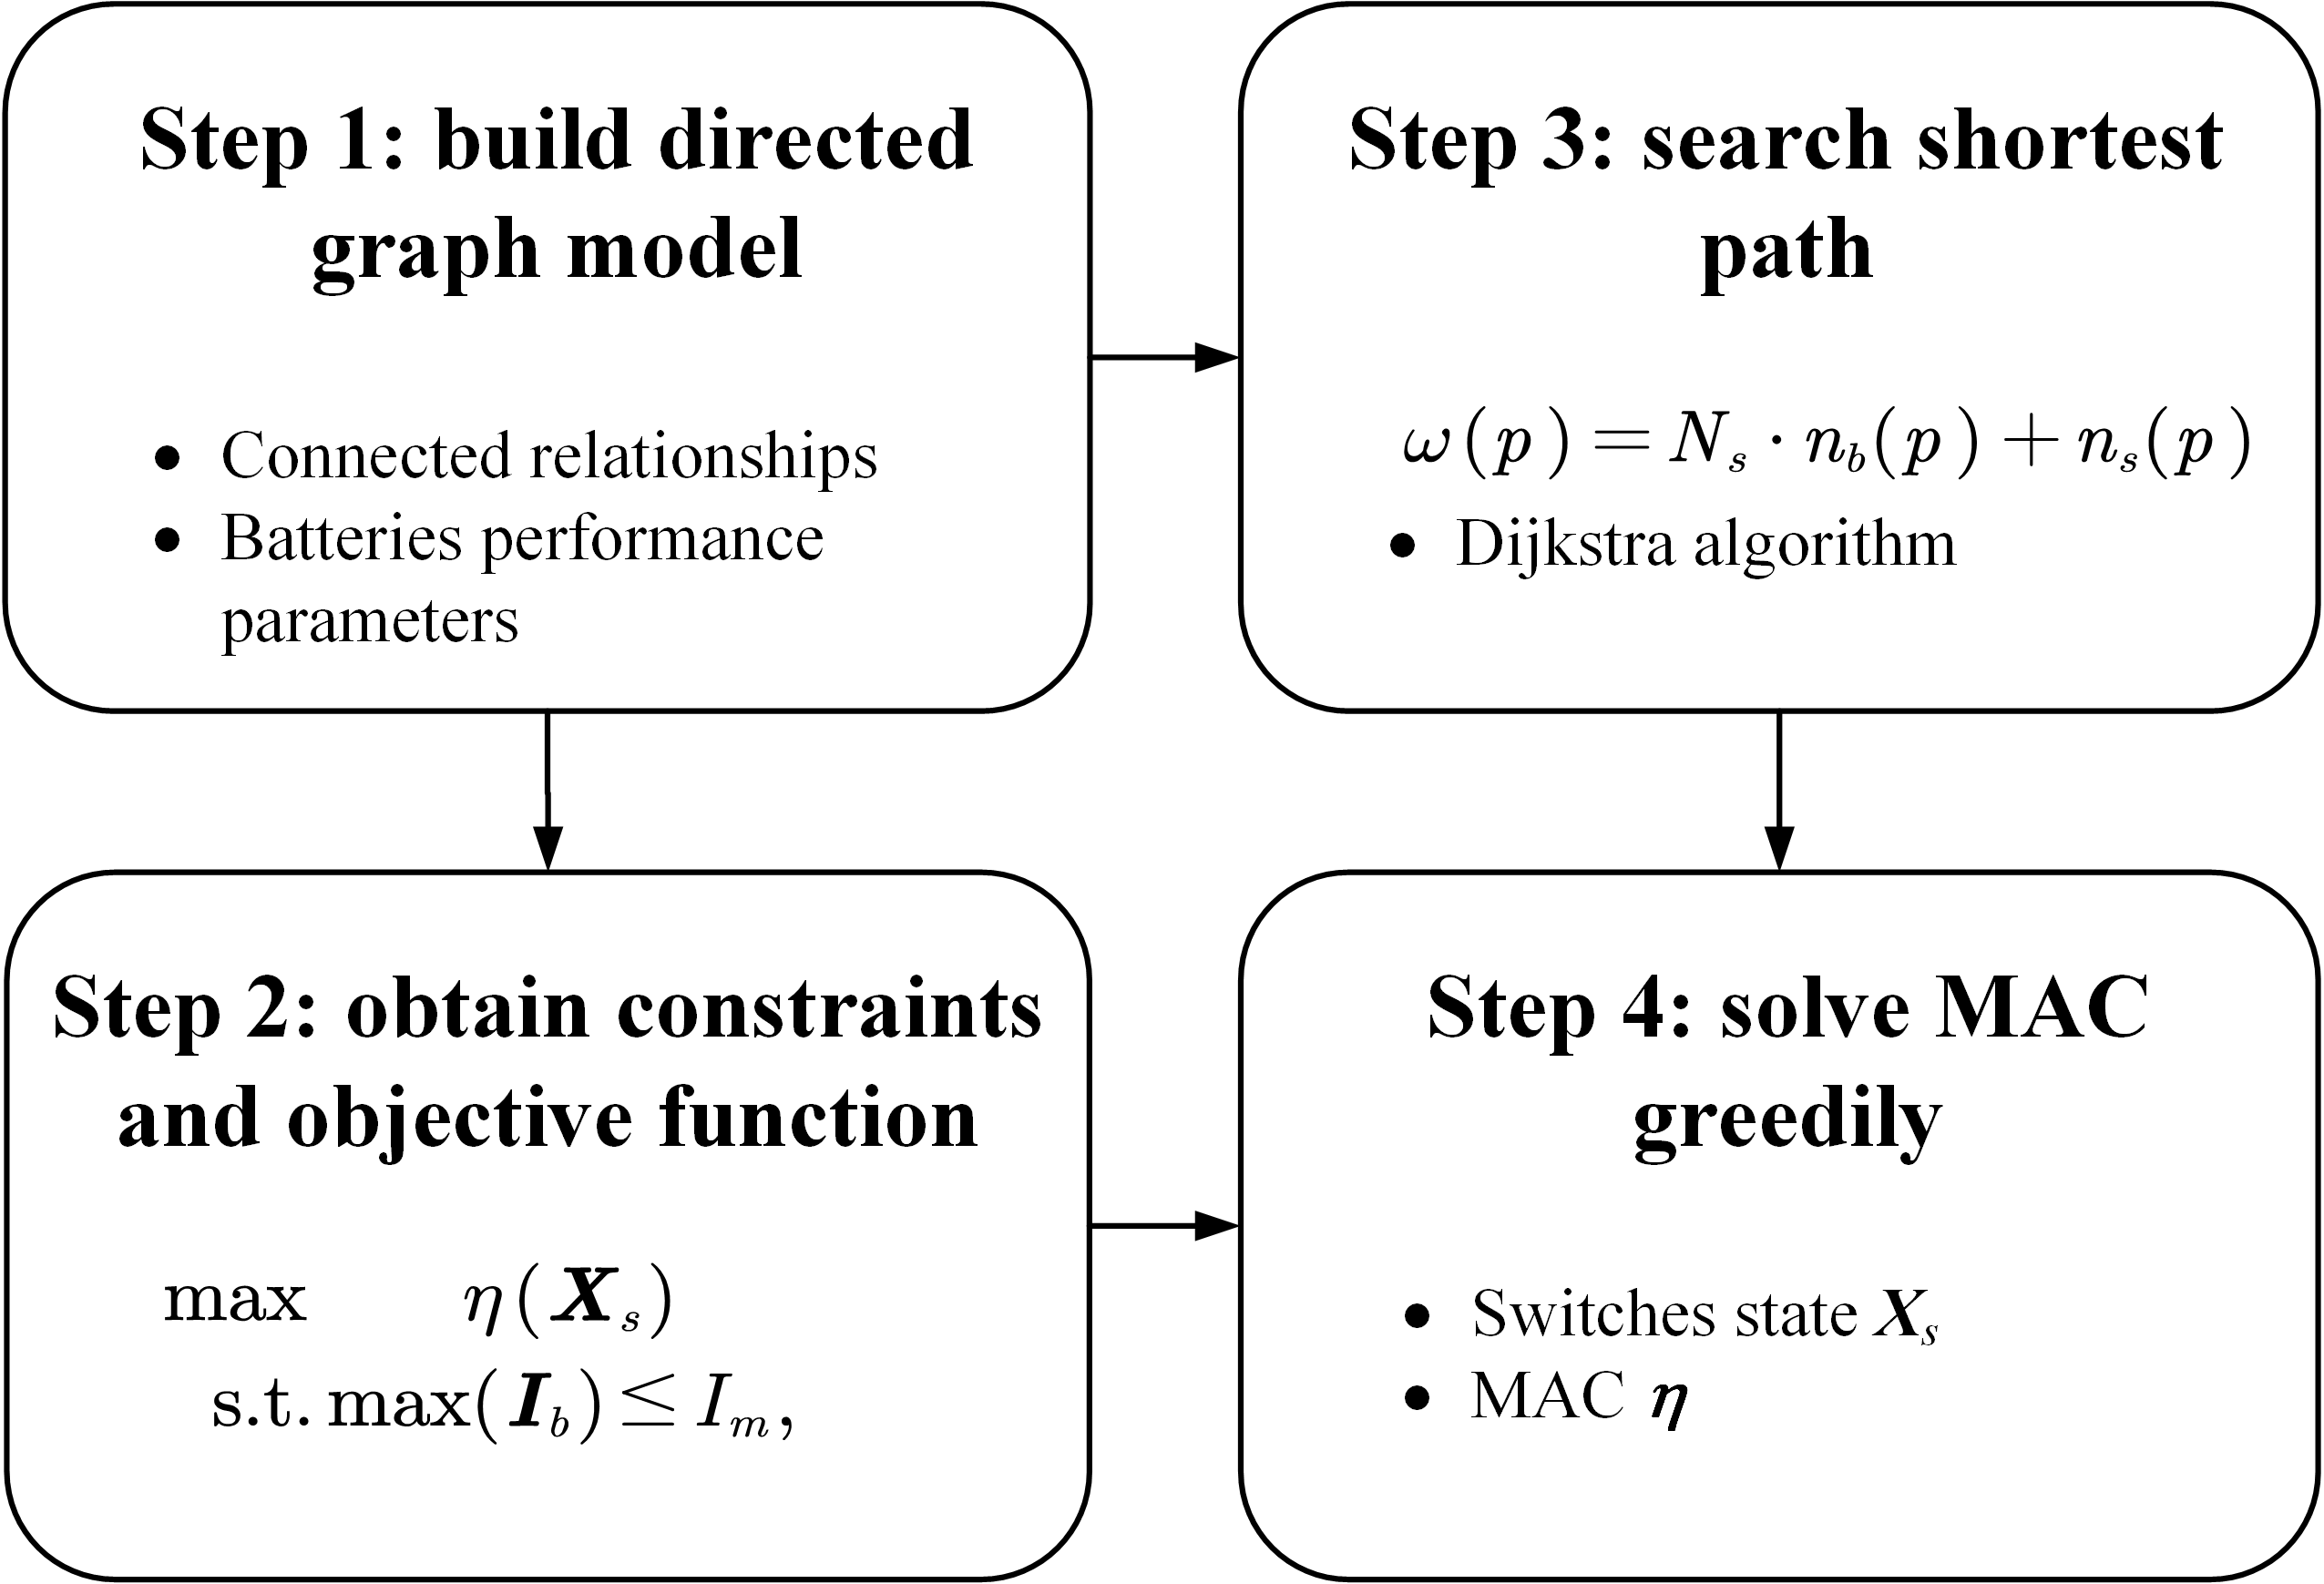
\includegraphics[width=\textwidth]{main.png}
    \end{subfigure}
    \caption{ 
        Diagram of this method, which contains four main steps.
    }
    \label{fig:main}
\end{figure}

\subsection{Directed graph \DIFdelbegin \DIFdel{Model}\DIFdelend \DIFaddbegin \DIFadd{model}\DIFaddend }

\begin{figure}[htbp]
    \centering
    \begin{subfigure}[b]{0.31\textwidth}
        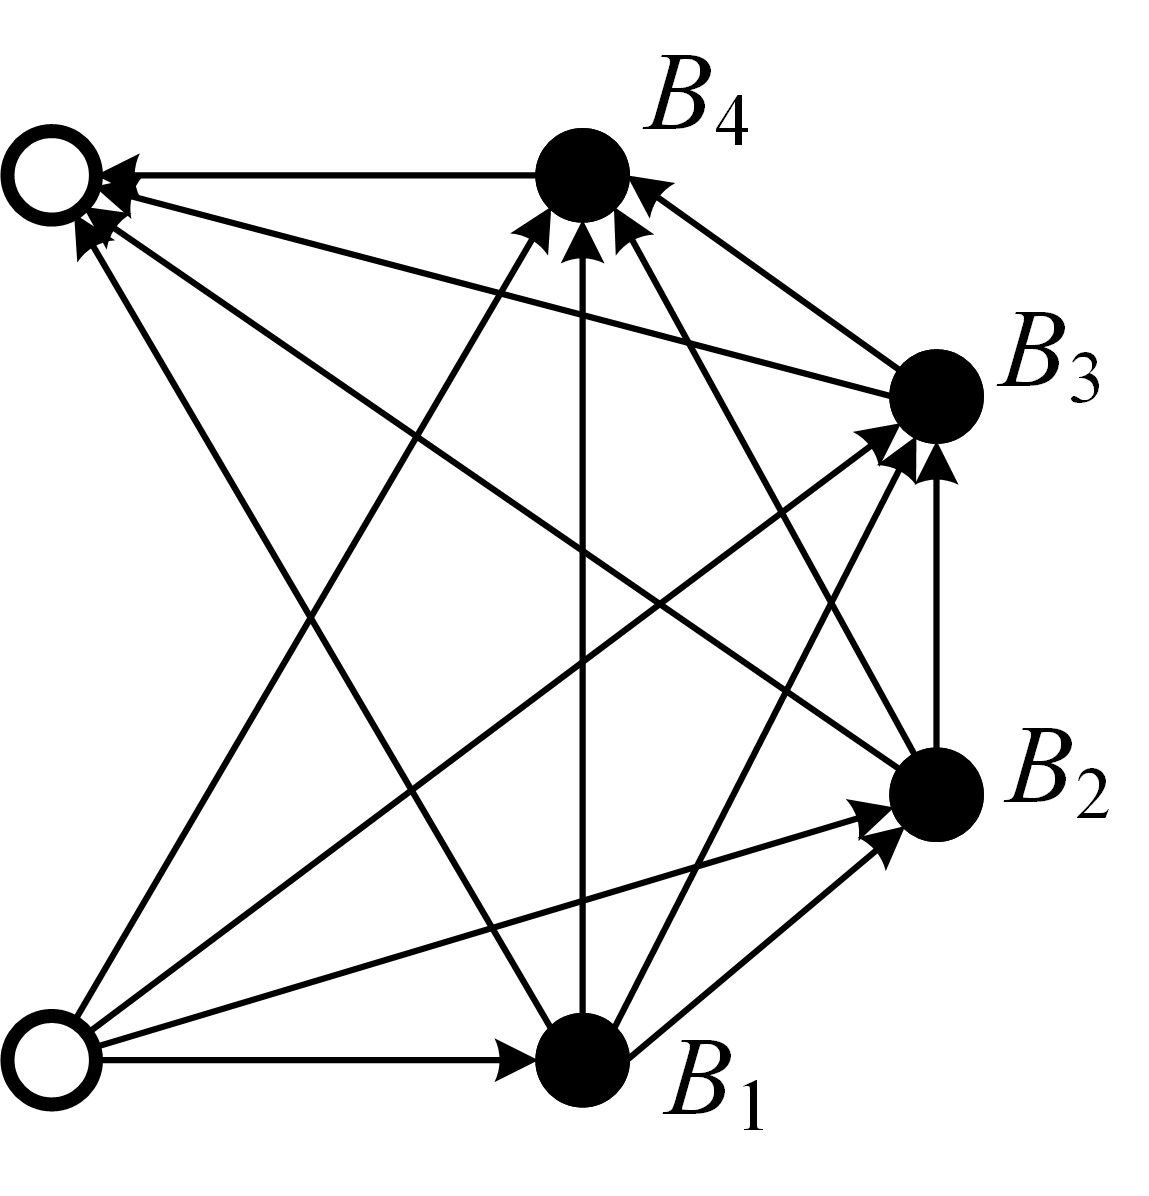
\includegraphics[width=\textwidth]{direct-graph-he.png}
        \caption{}
        \label{fig:direct-graph-he}
    \end{subfigure}
    \hspace{0.02\textwidth}
    \begin{subfigure}[b]{0.23\textwidth}
        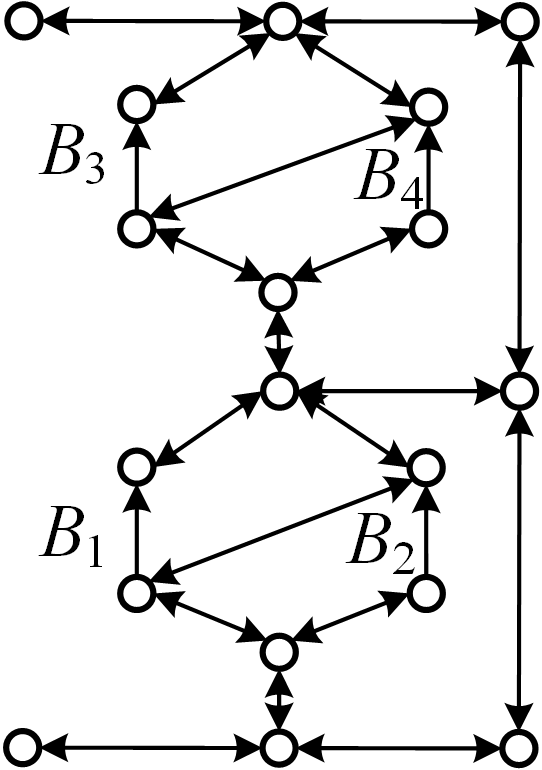
\includegraphics[width=\textwidth]{direct-graph-xu.png}
        \caption{}
        \label{fig:direct-graph-xu}
    \end{subfigure}
    \hspace{0.02\textwidth}
    \begin{subfigure}[b]{0.24\textwidth}
        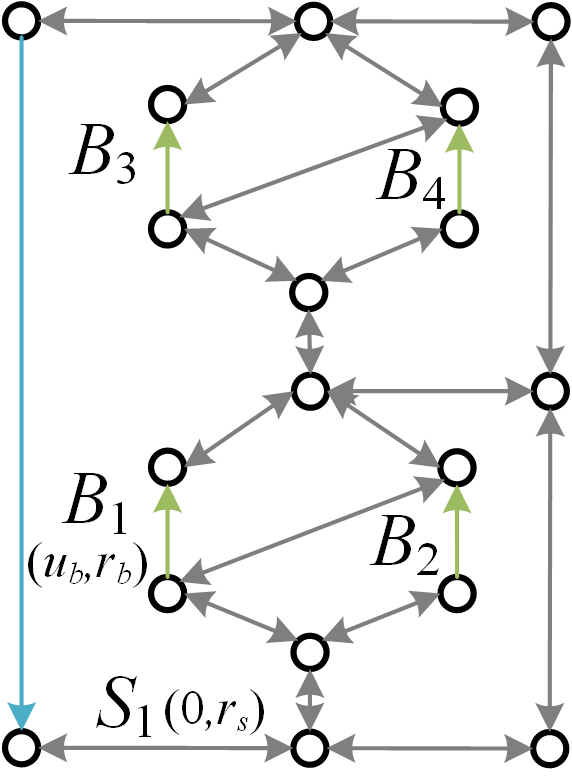
\includegraphics[width=\textwidth]{direct-graph-my.png}
        \caption{}
        \label{fig:direct-graph-my}
    \end{subfigure}
    \\
    \begin{subfigure}[b]{0.8\textwidth}
        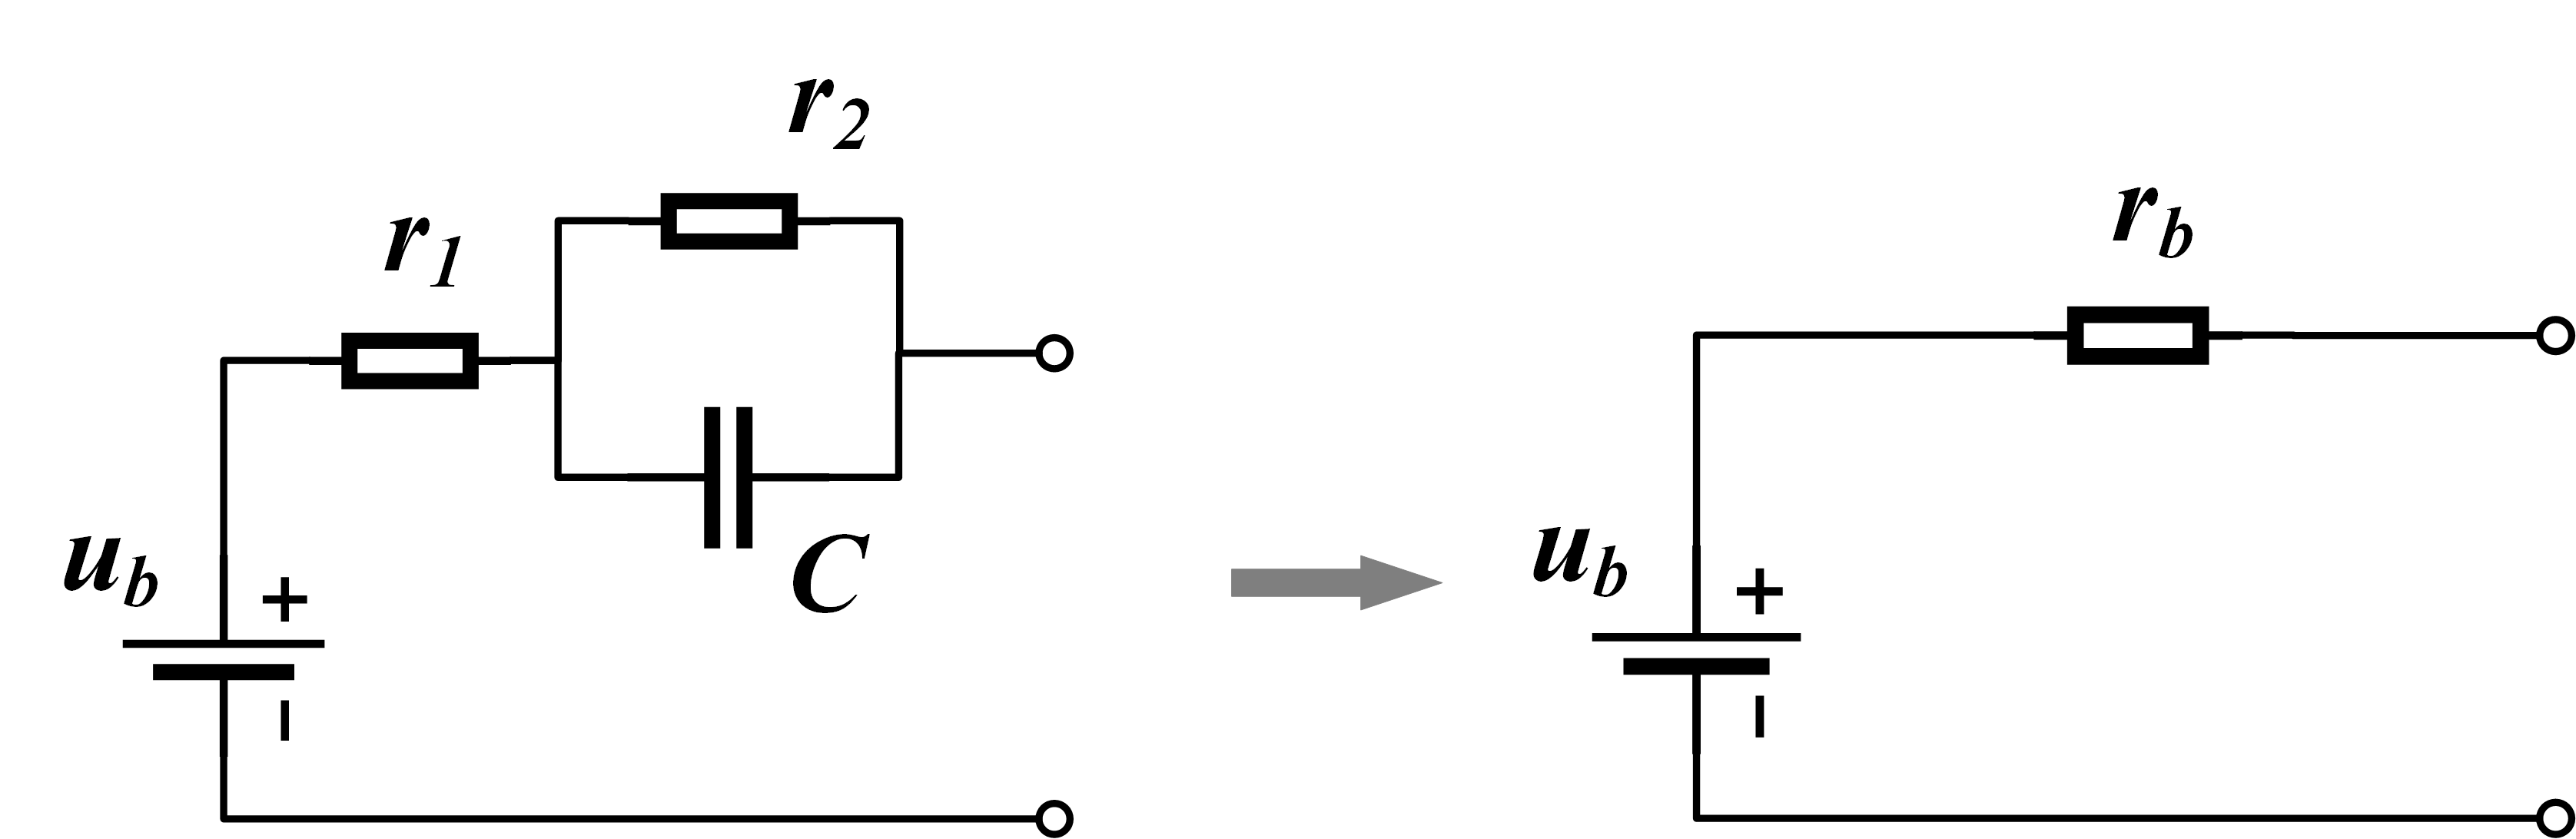
\includegraphics[width=\textwidth]{battery_simple.png}
        \caption{}
        \label{fig:battery_simple}
    \end{subfigure}
    \caption{ 
        Directed graph models used in (a) He's work \cite{heExploringAdaptiveReconfiguration2013}, (b) our previous work, and (c) \DIFdelbeginFL %DIFDELCMD < \added{the improved model in} %%%
\DIFdelendFL \DIFaddbeginFL \DIFaddFL{the improved model in }\DIFaddendFL this paper.
        (d) The equivalent circuit of a battery in this method.
    }
\end{figure}

He et al. \cite{heExploringAdaptiveReconfiguration2013} \DIFdelbegin \DIFdel{once }\DIFdelend proposed an abstracted directed graph model for \DIFaddbegin \DIFadd{an }\DIFaddend RBS, where the nodes \DIFdelbegin \DIFdel{represented }\DIFdelend \DIFaddbegin \DIFadd{represent }\DIFaddend the batteries, the edges \DIFdelbegin \DIFdel{represented }\DIFdelend \DIFaddbegin \DIFadd{represent }\DIFaddend the configuration flexibility, and the weight of each vertex \DIFdelbegin \DIFdel{corresponded }\DIFdelend \DIFaddbegin \DIFadd{corresponds }\DIFaddend to the battery voltage (\DIFdelbegin \DIFdel{Figure }\DIFdelend \DIFaddbegin \DIFadd{Fig. }\DIFaddend \ref{fig:direct-graph-he}). 
The model \DIFdelbegin \DIFdel{effectively captured }\DIFdelend \DIFaddbegin \DIFadd{captures }\DIFaddend all potential system configurations and \DIFdelbegin \DIFdel{offered }\DIFdelend \DIFaddbegin \DIFadd{offers }\DIFaddend a direct metric for configuration flexibility, but it \DIFdelbegin \DIFdel{did }\DIFdelend \DIFaddbegin \DIFadd{does }\DIFaddend not specify the physical implementation of the connectivity between batteries, meaning \DIFaddbegin \DIFadd{that }\DIFaddend one graph might \DIFdelbegin %DIFDELCMD < \replaced{correspond to}{have had} %%%
\DIFdelend \DIFaddbegin \DIFadd{correspond to }\DIFaddend multiple RBS structures.
We previously proposed a \DIFdelbegin \DIFdel{novel }\DIFdelend directed graph model that \DIFdelbegin \DIFdel{, }%DIFDELCMD < \replaced{completely different from}{in contrast to} %%%
\DIFdelend \DIFaddbegin \DIFadd{differs completely from }\DIFaddend He's model \DIFdelbegin \DIFdel{, used }\DIFdelend \DIFaddbegin \DIFadd{by using }\DIFaddend nodes to represent the connections between batteries and switches \DIFdelbegin \DIFdel{, }\DIFdelend and directed edges to represent batteries and switches (\DIFdelbegin \DIFdel{Figure }\DIFdelend \DIFaddbegin \DIFadd{Fig. }\DIFaddend \ref{fig:direct-graph-xu}), allowing for a one-to-one correspondence between the RBS structure and the directed graph model. 
This model \DIFdelbegin \DIFdel{was able to }\DIFdelend accurately and comprehensively \DIFdelbegin \DIFdel{represent }\DIFdelend \DIFaddbegin \DIFadd{represents }\DIFaddend the RBS topological structure but \DIFdelbegin \DIFdel{could not }\DIFdelend \DIFaddbegin \DIFadd{cannot }\DIFaddend be used for quantitative MAC calculations \DIFdelbegin \DIFdel{due to the lack of consideration }%DIFDELCMD < \replaced{on}{for} \replaced{the voltage, internal resistance and maximum allowable current of the battery}{battery and switch performance parameters}%%%
\DIFdelend \DIFaddbegin \DIFadd{because it does not consider  the voltage, internal resistance, and MAC of the battery}\DIFaddend . 
To address this \DIFdelbegin \DIFdel{, an }%DIFDELCMD < \replaced{improvement on our previous model is conducted by}{improved directed graph model is used here based on our original model,} %%%
\DIFdelend \DIFaddbegin \DIFadd{issue, we improve our previous model by }\DIFaddend adding electromotive force and resistance attributes on the edges based \DIFdelbegin %DIFDELCMD < \replaced{on its}{to} %%%
\DIFdel{equivalent circuits}%DIFDELCMD < \deleted{(Figure \ref{fig:direct-graph-my})}%%%
\DIFdelend \DIFaddbegin \DIFadd{on its equivalent circuits}\DIFaddend .
The model also considers the external load as an equivalent resistance and \DIFdelbegin \DIFdel{integrate }\DIFdelend \DIFaddbegin \DIFadd{integrates }\DIFaddend it into the analysis, making it a complete circuit model for later circuit \DIFdelbegin \DIFdel{analysis.
}%DIFDELCMD < \added{Figure \ref{fig:direct-graph-my} shows the improved directed graph model used in this paper.}
%DIFDELCMD < %%%
\DIFdel{The following  will provide }\DIFdelend \DIFaddbegin \DIFadd{analyses.
Fig. \ref{fig:direct-graph-my} shows the improved directed graph model used in this paper.
The following  provides }\DIFaddend a detailed explanation of the method for equating \DIFdelbegin \DIFdel{the components in RBS }\DIFdelend \DIFaddbegin \DIFadd{components in RBSs }\DIFaddend and constructing the directed graph model.


\DIFdelbegin \DIFdel{In order to }\DIFdelend \DIFaddbegin \DIFadd{To }\DIFaddend use circuit analysis methods to solve the MAC of the RBS, the components in the RBS are equated to ideal circuit elements.
\DIFdelbegin %DIFDELCMD < \added{For instance,} \replaced{a}{A}%%%
\DIFdel{s shown in Figure }\DIFdelend \DIFaddbegin \DIFadd{For instance, as shown in Fig. }\DIFaddend \ref{fig:battery_simple}, the battery in the RBS can be represented as a black-box circuit consisting of two resistors \DIFdelbegin \DIFdel{(i.e., }\DIFdelend $r_1$ and $r_2$ \DIFdelbegin \DIFdel{) }\DIFdelend and a capacitor  \DIFdelbegin \DIFdel{(i.e., }\DIFdelend $C$\DIFdelbegin \DIFdel{)}\DIFdelend , known as the Thevenin model \cite{hongwenheStateofChargeEstimationLithiumIon2011,mousavig.VariousBatteryModels2014}.
With an emphasis on the stable output of the RBS, the capacitor in the Thevenin model can be considered as an open circuit without affecting the steady-state current.
Therefore,  \DIFdelbegin \DIFdel{the }\DIFdelend battery $i$ in the RBS can be simplified as \DIFdelbegin \DIFdel{the }\DIFdelend \DIFaddbegin \DIFadd{a }\DIFaddend series connection between a constant voltage source $u_{i}$ and a resistor $r_{i}$.
Furthermore, the state of switch $j$ in the RBS is represented by a binary variable $x_j$, where 0 is \DIFdelbegin \DIFdel{for }\DIFdelend ON and 1 is \DIFdelbegin \DIFdel{for OFF, respectively}\DIFdelend \DIFaddbegin \DIFadd{OFF}\DIFaddend .
When the switch is closed, \DIFdelbegin \DIFdel{it }\DIFdelend \DIFaddbegin \DIFadd{the circuit }\DIFaddend can be regarded as a resistor with a very small resistance \DIFdelbegin \DIFdel{value }\DIFdelend $r_{j}$.
\DIFdelbegin \DIFdel{Lastly}\DIFdelend \DIFaddbegin \DIFadd{Finally}\DIFaddend , the external load is considered as a resistor with \DIFdelbegin \DIFdel{a value of }\DIFdelend \DIFaddbegin \DIFadd{resistance }\DIFaddend $R_o$.


For a given RBS structure, \DIFdelbegin %DIFDELCMD < \replaced{its directed graph model $G(V,E)$ is constructed as follows:}{the directed graph model for the RBS is constructed as a directed graph $G(V,E)$ in such a way that:}
%DIFDELCMD < %%%
\DIFdelend \DIFaddbegin \DIFadd{its directed graph model $G(V,E)$ is constructed as follows:
}\DIFaddend \begin{enumerate}
    \item Nodes:
        The nodes in the directed graph correspond to the connection points of components in the actual RBS. 
        Assuming there are a total of $N$ nodes in the RBS, for the sake of convenience, the anode of the RBS is denoted as $v_1$ and the cathode as $v_N$.
    \item Edges:
        The edges in the directed graph correspond to the batteries, switches, and external electrical loads in the actual RBS.
        Therefore, there are three types of directed edges. 
        For a battery $B_i$, its directed edge $e_i$ is drawn from the cathode to the anode \DIFdelbegin \DIFdel{, as the battery }\DIFdelend \DIFaddbegin \DIFadd{because the battery in operation }\DIFaddend only allows current to flow in one direction\DIFdelbegin \DIFdel{when in operation}\DIFdelend .
        For a switch $S_j$, since it is allowed to work under bi-directional currents, it is represented by a pair of directed edges with two-way directions. 
        Regarding the external electronic load, \DIFdelbegin \DIFdel{as }\DIFdelend \DIFaddbegin \DIFadd{because }\DIFaddend it is connected to the anode and cathode of the RBS, a directed edge from $v_N$ to $v_1$  \DIFdelbegin \DIFdel{is used to represent }\DIFdelend \DIFaddbegin \DIFadd{represents }\DIFaddend it. 
        In conclusion, for a given RBS structure with $N_b$ batteries and $N_s$ switches, the \DIFdelbegin \DIFdel{total }\DIFdelend number of directed edges is $N_b+2N_s+1$, where 1 refers to the external electrical load.
    \item \DIFdelbegin \DIFdel{Edges' attributes}\DIFdelend \DIFaddbegin \DIFadd{Attributes of edges}\DIFaddend :
        Each edge is assigned two attributes, voltage difference and resistance, based on the equivalent method mentioned above.
        The values for  \DIFdelbegin \DIFdel{the }\DIFdelend battery $B_i$, switch $S_j$, and external loads correspond to $(u_i, r_i)$, $(0, r_j)$, and $(0, R_o)$, respectively.
\end{enumerate}

\subsection{Constraints and \DIFdelbegin \DIFdel{Objective Function}\DIFdelend \DIFaddbegin \DIFadd{objective function}\DIFaddend }

\DIFdelbegin %DIFDELCMD < \replaced{For a given RBS, determination of its MAC}{Based on the definition of MAC, determining the MAC of RBS} %%%
\DIFdelend \DIFaddbegin \DIFadd{For a given RBS, determining its MAC }\DIFaddend involves maximizing the RBS output current while ensuring that the \DIFaddbegin \DIFadd{sum of the }\DIFaddend currents of all batteries \DIFdelbegin \DIFdel{do }\DIFdelend \DIFaddbegin \DIFadd{does }\DIFaddend not exceed the batteries' \DIFdelbegin \DIFdel{maximum allowable current. 
In this subsection , }\DIFdelend \DIFaddbegin \DIFadd{MAC. 
This subsection establishes }\DIFaddend the constraints and objective function to \DIFdelbegin \DIFdel{solve }\DIFdelend \DIFaddbegin \DIFadd{determine }\DIFaddend the RBS's MAC  \DIFdelbegin \DIFdel{will be established }\DIFdelend through circuit analysis \DIFdelbegin \DIFdel{, based on }%DIFDELCMD < \replaced{its directed graph model provided in the previous subsection}{the previously constructed directed graph model}%%%
\DIFdelend \DIFaddbegin \DIFadd{based on the directed graph model provided in the previous section}\DIFaddend .


First, the topology in the directed graph model is represented in matrix form $\bm{A}$, known as the incidence matrix \DIFdelbegin \DIFdel{, }%DIFDELCMD < \replaced{defined}{to facilitate circuit analysis.
%DIFDELCMD < The specific definition of the incidence matrix is shown} %%%
\DIFdel{in Equation \ref{eq:A}.
}\DIFdelend \DIFaddbegin \DIFadd{and defined as follows:
}\DIFaddend \begin{align}\label{eq:A}
    a_{kl}=
    \begin{cases}
        1,  & \text{edge $l$ leaves node $k$},\\
        -1, & \text{edge $l$ enters node $k$},\\
        0,  & \text{otherwise}.
    \end{cases}
\end{align}
For a directed graph consisting of $N$ nodes and $N_b+2N_s+1$ directed edges, its incidence matrix $\bm{A}$ is an $N\times(N_b+2N_s+1)$ matrix. 
In this matrix, the rows and columns represent the nodes and edges of the directed graph, respectively.
By distinguishing the components in the RBS corresponding to each column, $\bm{A}$ can be rewritten as
\DIFdelbegin \DIFdel{:
}\DIFdelend \begin{equation}\label{eq:A_bso}
    \bm{A} =
    \begin{bmatrix}
        \bm{A}_b & \bm{A}_s & \bm{A}_o
    \end{bmatrix},
\end{equation}
where $\bm{A}_b$, $\bm{A}_s$\DIFaddbegin \DIFadd{, }\DIFaddend and $\bm{A}_o$ are the sub-matrices corresponding to the batteries, switches\DIFaddbegin \DIFadd{, }\DIFaddend and external electrical load, respectively.
To \DIFdelbegin \DIFdel{alleviate }\DIFdelend \DIFaddbegin \DIFadd{reduce the }\DIFaddend computational complexity, \DIFaddbegin \DIFadd{the dimensions of }\DIFaddend matrix $\bm{A}$ \DIFdelbegin \DIFdel{undergoes dimensionality reduction}\DIFdelend \DIFaddbegin \DIFadd{are reduced}\DIFaddend .
Since each directed edge has one node to leave and one to enter, the \DIFdelbegin \DIFdel{sum of the }\DIFdelend values in every column of $\bm{A}$ \DIFdelbegin \DIFdel{is }\DIFdelend \DIFaddbegin \DIFadd{sum to }\DIFaddend zero.
Therefore\DIFdelbegin \DIFdel{removing }%DIFDELCMD < \replaced{the last}{any single one} %%%
\DIFdelend \DIFaddbegin \DIFadd{, removing the last }\DIFaddend row will not result in a loss of information. 
\DIFdelbegin %DIFDELCMD < \deleted{Without loss of generality, the last row is removed here.}
%DIFDELCMD < %%%
\DIFdel{On the other hand}\DIFdelend \DIFaddbegin \DIFadd{Conversely}\DIFaddend , since each switch in the RBS is represented by a pair of directed edges with two-way directions, the two columns corresponding to the switch are mutually opposite.
Thus, for the \DIFdelbegin \DIFdel{sub-matrix }\DIFdelend \DIFaddbegin \DIFadd{submatrix }\DIFaddend $\bm{A}_s$, only one column is retained for each pair of columns representing the same switch.
As a result, $\bm{A}$ can be reduced to \DIFdelbegin \DIFdel{a }\DIFdelend \DIFaddbegin \DIFadd{an }\DIFaddend $(N-1)\times(N_b+N_s+1)$ matrix, denoted  \DIFdelbegin \DIFdel{as }\DIFdelend $\bm{\tilde{A}}$, for further calculation of current and voltage.
Similar to \DIFdelbegin \DIFdel{Equation \ref{eq:A_bso}}\DIFdelend \DIFaddbegin \DIFadd{Eq. (\ref{eq:A_bso})}\DIFaddend , $\bm{\tilde{A}}$ can be rewritten as
\DIFdelbegin \DIFdel{:
}\DIFdelend \begin{equation}\label{eq:A_bso_tilde}
    \bm{\tilde{A}} =
    \begin{bmatrix}
        \bm{\tilde{A}}_b & \bm{\tilde{A}}_s & \bm{\tilde{A}}_o
    \end{bmatrix}.
\end{equation}


After obtaining the incidence matrix, the currents of all batteries and output in \DIFaddbegin \DIFadd{the }\DIFaddend RBS are determined by solving the circuit equations.
According to \DIFdelbegin \DIFdel{Kirchhoffs }\DIFdelend \DIFaddbegin \DIFadd{Kirchhoff's }\DIFaddend law, we have
\begin{align}\label{eq:Kirchhoffs_law}
    \begin{cases}
        \bm{\tilde{A}} \bm{I} = \bm{0}, \\
        \bm{U}        = \bm{\tilde{A}}^\T \bm{U}_n,
    \end{cases}
\end{align}
where $\bm{I}$ and $\bm{U}$ indicate the current and voltage difference arrays of the $N_b+N_s+1$ edges, respectively\DIFdelbegin \DIFdel{;
}\DIFdelend \DIFaddbegin \DIFadd{, and
}\DIFaddend $\bm{U}_n$ is the voltage array of the $N-1$ nodes.
These directed edges are treated as generalized branches and expressed in matrix form as follows\DIFaddbegin \DIFadd{:
}\DIFaddend \begin{equation}\label{eq:generalized_branches}
    \bm{I} = \bm{Y}\bm{X} \bm{U} - \bm{Y}\bm{X} \bm{U}_s +\bm{I}_s,
\end{equation}
where $\bm{U}_s$ and $\bm{I}_s$ denote the source voltage and source current of the generalized branches, respectively.
Because all batteries have been equivalent to voltage sources rather than current sources in the previous \DIFdelbegin \DIFdel{subsection}\DIFdelend \DIFaddbegin \DIFadd{section}\DIFaddend , all elements of the array $\bm{I}_s$ are \DIFdelbegin \DIFdel{0, 
while }\DIFdelend \DIFaddbegin \DIFadd{zero, 
whereas }\DIFaddend the elements of the array $\bm{U}_s$ are equal to the first attribute of the corresponding edges in the directed graph.
The \DIFaddbegin \DIFadd{matrix }\DIFaddend $\bm{Y}$ in \DIFdelbegin %DIFDELCMD < \added{Equation} %%%
\DIFdel{\ref{eq:generalized_branches}}\DIFdelend \DIFaddbegin \DIFadd{Eq. (\ref{eq:generalized_branches}) }\DIFaddend is the admittance matrix of the circuit \DIFdelbegin \DIFdel{, }\DIFdelend \DIFaddbegin \DIFadd{and is }\DIFaddend defined as the inverse of the impedance matrix.
\DIFdelbegin %DIFDELCMD < \replaced{The}{That is the} %%%
\DIFdel{elements }%DIFDELCMD < \replaced{on}{of} %%%
\DIFdel{the diagonal }%DIFDELCMD < \added{of} %%%
\DIFdelend \DIFaddbegin \DIFadd{The elements on the diagonal of }\DIFaddend matrix $\bm{Y}$ are equal to the reciprocal of \DIFdelbegin %DIFDELCMD < \added{the resistance, which is} %%%
\DIFdel{the }\DIFdelend \DIFaddbegin \DIFadd{the resistance, which is the }\DIFaddend second attribute of the corresponding edges in the directed graph\DIFdelbegin \DIFdel{, and the }\DIFdelend \DIFaddbegin \DIFadd{. The }\DIFaddend off-diagonal elements \DIFdelbegin %DIFDELCMD < \added{$\bm{Y}$} %%%
\DIFdel{are 0.
The }\DIFdelend \DIFaddbegin \DIFadd{of $\bm{Y}$ are zero.
}\DIFaddend $\bm{X}$ is the state matrix \DIFdelbegin \DIFdel{, which describes }\DIFdelend \DIFaddbegin \DIFadd{that determines }\DIFaddend whether the RBS batteries and switches \DIFdelbegin \DIFdel{are allowed to }\DIFdelend \DIFaddbegin \DIFadd{can }\DIFaddend pass current.
It is defined as
\begin{equation}\label{eq:X}
    \bm{X} = \diag(
    \DIFdelbegin %DIFDELCMD < \underbrace{1, 0 \cdots, 1}%%%
\DIFdelend \DIFaddbegin \underbrace{1, 0, \dots, 1}\DIFaddend _{N_b~\text{of}~0/1},
    \DIFdelbegin %DIFDELCMD < \underbrace{1, 0 \cdots, 1}%%%
\DIFdelend \DIFaddbegin \underbrace{1, 0, \dots, 1}\DIFaddend _{N_s~\text{of}~0/1},
    1)
    =\begin{bmatrix}
        \bm{X}_b & & \\
        & \bm{X}_s &\\
        & & 1
    \end{bmatrix}\DIFdelbegin \DIFdel{.
}\DIFdelend \DIFaddbegin \DIFadd{,
}\DIFaddend \end{equation}
\DIFdelbegin \DIFdel{Where the elements }\DIFdelend \DIFaddbegin \DIFadd{where element }\DIFaddend $x_i$ of \DIFdelbegin \DIFdel{the }\DIFdelend matrix $\bm{X}_b$ \DIFdelbegin \DIFdel{represent whether the }\DIFdelend \DIFaddbegin \DIFadd{indicates whether }\DIFaddend battery $i$ has been removed from the circuit, with $x_i=1$ indicating removal and $x_i=0$ indicating that \DIFdelbegin \DIFdel{it }\DIFdelend \DIFaddbegin \DIFadd{battery $i$ }\DIFaddend is still available to supply power. 
When all batteries are \DIFdelbegin \DIFdel{health }\DIFdelend \DIFaddbegin \DIFadd{healthy }\DIFaddend and capable of providing current to the external load, $\bm{X}_b$ is \DIFdelbegin \DIFdel{an }\DIFdelend \DIFaddbegin \DIFadd{the }\DIFaddend identity matrix. 
The elements $x_j$ of  \DIFdelbegin \DIFdel{the }\DIFdelend matrix $\bm{X}_s$ \DIFdelbegin \DIFdel{represent whether the }\DIFdelend \DIFaddbegin \DIFadd{determine whether }\DIFaddend switch $j$ is closed, with $x_j=1$ indicating \DIFdelbegin \DIFdel{closure }\DIFdelend \DIFaddbegin \DIFadd{a closed switch }\DIFaddend and $x_j=0$ indicating \DIFdelbegin \DIFdel{disconnection}\DIFdelend \DIFaddbegin \DIFadd{an open switch}\DIFaddend , which is consistent with the previous \DIFdelbegin \DIFdel{subsection}\DIFdelend \DIFaddbegin \DIFadd{section}\DIFaddend .


Theoretically, the output current $I_o$ and the currents of each battery $\bm{I}_b$ in the RBS  can be determined by solving \DIFdelbegin \DIFdel{Equations \ref{eq:Kirchhoffs_law}, \ref{eq:generalized_branches}, and \ref{eq:X}}\DIFdelend \DIFaddbegin \DIFadd{Eqs. (\ref{eq:Kirchhoffs_law})--(\ref{eq:X}) }\DIFaddend under any given state $\bm{X}$.
\DIFdelbegin \DIFdel{In order to }\DIFdelend \DIFaddbegin \DIFadd{To }\DIFaddend obtain specific constraint conditions and objective functions, it is further assumed that all batteries have the same electromotive force and internal resistance, \DIFdelbegin \DIFdel{denoted as }\DIFdelend \DIFaddbegin \DIFadd{which are denoted }\DIFaddend $u_b$ and $r_b$, respectively.
This allows \DIFdelbegin \DIFdel{for the derivation of }\DIFdelend \DIFaddbegin \DIFadd{us to derive }\DIFaddend explicit expressions for $I_o$ and $\bm{I}_b$.
After derivation and simplification, the output current $I_o$ and the currents of each battery $\bm{I}_b$ are ultimately represented as \DIFdelbegin \DIFdel{Equations \ref{eq:I_o}and \ref{eq:I_b}, respectively.
}\begin{displaymath}\DIFdel{\label{eq:I_o}
    I_o = \frac{1}{R_o r_b} \bm{\tilde{A}}_o^\T \bm{Y}_n^{-1}(\bm{X}) \bm{\tilde{A}}_b \bm{U}_b,
}\end{displaymath}%DIFAUXCMD
\DIFdelend \DIFaddbegin \DIFadd{Eqs. (\ref{eq:I_o}) and (\ref{eq:I_b}), respectively:
}\begin{eqnarray}\DIFadd{\label{eq:I_o}
    I_o }&\DIFadd{=}& \DIFadd{\frac{1}{R_o r_b} \bm{\tilde{A}}_o^\T \bm{Y}_n^{-1}(\bm{X}) \bm{\tilde{A}}_b \bm{U}_b,
}\\\DIFadd{\label{eq:I_b}
    \bm{I}_b }&\DIFadd{=}& \DIFadd{\frac{1}{r_b^2}[\bm{\tilde{A}}_b^\T \bm{Y}_n^{-1}(\bm{X}) \bm{\tilde{A}}_b\bm{U}_b -r_b \bm{U}_b],
}\end{eqnarray}\DIFaddend 
\DIFdelbegin \begin{displaymath}\DIFdel{\label{eq:I_b}
    \bm{I}_b = \frac{1}{r_b^2}[\bm{\tilde{A}}_b^\T \bm{Y}_n^{-1}(\bm{X}) \bm{\tilde{A}}_b\bm{U}_b -r_b \bm{U}_b],
}\end{displaymath}%DIFAUXCMD
\DIFdelend where $\bm{U}_b$ is \DIFdelbegin \DIFdel{a }\DIFdelend \DIFaddbegin \DIFadd{an }\DIFaddend $N_b\times 1$ array with all elements \DIFdelbegin \DIFdel{equaling }\DIFdelend \DIFaddbegin \DIFadd{equal }\DIFaddend to $u_b$\DIFdelbegin \DIFdel{;
}\DIFdelend \DIFaddbegin \DIFadd{,
and }\DIFaddend $\bm{Y}_n$ is the equivalent admittance matrix of the circuit \DIFdelbegin \DIFdel{, }\DIFdelend \DIFaddbegin \DIFadd{and is }\DIFaddend defined as
\begin{equation}\label{eq:Yn}
    \bm{Y}_n (\bm{X}) = \frac{1}{R_o} \bm{\tilde{A}}_o\bm{\tilde{A}}_o^\T + \frac{1}{r_b} \bm{\tilde{A}}_b\bm{X}_b\bm{\tilde{A}}_b^\T + \frac{1}{r_s}\bm{\tilde{A}}_s\bm{X}_s\bm{\tilde{A}}_s^\T.
\end{equation}


To characterize the current output capacity of the RBS structure under different switching states, an indicator $\eta$ is defined by the ratio of $I_o$ \DIFdelbegin \DIFdel{and }\DIFdelend \DIFaddbegin \DIFadd{to }\DIFaddend $\max (\bm{I}_b)$\DIFdelbegin \DIFdel{shown in Equation \ref{eq:eta}}\DIFdelend :
\begin{equation}\label{eq:eta}
    \eta = \frac{I_o}{\max (\bm{I}_b)}.
\end{equation}
Finally the problem of \DIFdelbegin \DIFdel{solving }\DIFdelend \DIFaddbegin \DIFadd{finding the }\DIFaddend MAC can be formulated as
\begin{align}
    & \max \eta(\bm{X}_s) \label{eq:max_eta}\\
    \DIFdelbegin \DIFdel{\text{s.t.} }\DIFdelend \DIFaddbegin \DIFadd{\text{s.t. } }\DIFaddend & \max (\bm{I}_b) \leq I_m, \label{eq:Ib_leq_Im}
\end{align}
where $I_m$ is the \DIFdelbegin \DIFdel{maximum allowable current }\DIFdelend \DIFaddbegin \DIFadd{MAC }\DIFaddend of the battery.


However, it \DIFdelbegin \DIFdel{is }%DIFDELCMD < \added{still} %%%
\DIFdelend \DIFaddbegin \DIFadd{remains }\DIFaddend computationally difficult to solve \DIFdelbegin \DIFdel{\ref{eq:max_eta} because of the }\DIFdelend \DIFaddbegin \DIFadd{Eq. (\ref{eq:max_eta}) because of }\DIFaddend $\bm{Y}_n^{-1}$.
On one hand,  \DIFdelbegin \DIFdel{due to }\DIFdelend the introduction of nonlinear terms by $\bm{Y}_n^{-1}$ \DIFdelbegin \DIFdel{, many  effective }\DIFdelend \DIFaddbegin \DIFadd{renders many  }\DIFaddend methods in linear optimization \DIFdelbegin \DIFdel{are not suitable for this }%DIFDELCMD < \replaced{scenario}{problem}%%%
\DIFdelend \DIFaddbegin \DIFadd{unsuitable for this problem}\DIFaddend .
On the other hand, the rank of $Y_{n}$ is proportional to the number of batteries and switches, which can be very large for a large RBS\DIFdelbegin \DIFdel{system}\DIFdelend , leading to \DIFaddbegin \DIFadd{a }\DIFaddend significant computational burden.
\DIFdelbegin \DIFdel{Therefore}\DIFdelend \DIFaddbegin \DIFadd{As a result}\DIFaddend , intelligent algorithms that rely on \DIFdelbegin \DIFdel{evolving }\DIFdelend \DIFaddbegin \DIFadd{evolution }\DIFaddend by iteration may face efficiency \DIFdelbegin %DIFDELCMD < \replaced{problem}{issues} %%%
\DIFdelend \DIFaddbegin \DIFadd{problems }\DIFaddend when dealing with \DIFdelbegin \DIFdel{large RBS system.
In order to }\DIFdelend \DIFaddbegin \DIFadd{a large RBS.
To }\DIFaddend address this issue, the problem should be considered from the perspective of guiding the RBS to reconstruct as many parallel structures as possible.
Consequently, a greedy algorithm based on the shortest path is proposed. 
The detailed implementation \DIFdelbegin \DIFdel{process }\DIFdelend \DIFaddbegin \DIFadd{of this algorithm }\DIFaddend is presented in the following two \DIFdelbegin \DIFdel{subsections}\DIFdelend \DIFaddbegin \DIFadd{sections}\DIFaddend .

\subsection{Shortest \DIFdelbegin \DIFdel{Path}\DIFdelend \DIFaddbegin \DIFadd{path}\DIFaddend }

The path $p$ used in this method is defined as the complete route that passes through one battery (or a consecutive series of batteries) and closed switches, connecting the anode $v_1$ to the cathode $v_N$ of the RBS.
By applying a penalty to the series-connected batteries on the path, where additional batteries imply a \DIFdelbegin \DIFdel{longer }\DIFdelend \DIFaddbegin \DIFadd{greater }\DIFaddend distance, the algorithm encourages the RBS to form parallel structures \DIFdelbegin \DIFdel{as much as possible.
Meanwhile}\DIFdelend \DIFaddbegin \DIFadd{to the extent possible.
In addition}\DIFaddend , to reduce the number of switches controlled during the reconstruction process, a penalty is also applied to the total number of switches on the path \DIFdelbegin \DIFdel{, }\DIFdelend while ensuring the minimum number of batteries.
Therefore, the distance $\omega$ of \DIFdelbegin \DIFdel{the }\DIFdelend path $p$ is  
\DIFdelbegin \DIFdel{defined by the following equation: 
}\DIFdelend \begin{equation}\label{eq:weight}
    \omega(p) = N_s  \DIFdelbegin \DIFdel{\cdot }\DIFdelend n_b (p) + n_s (p),
\end{equation}
where $N_s$ is the total number of switches in the system\DIFdelbegin \DIFdel{; 
}\DIFdelend \DIFaddbegin \DIFadd{, 
and }\DIFaddend $n_b(p)$ and $n_s(p)$ are number of batteries and switches in \DIFdelbegin \DIFdel{the }\DIFdelend path $p$\DIFaddbegin \DIFadd{, }\DIFaddend respectively. 
Moreover, the shortest path $SP_i$ is defined as the path with the minimum $\omega$ for battery $i$\DIFdelbegin \DIFdel{, as shown in the following equation}\DIFdelend :
\begin{equation}\label{eq:def_sp}
    SP_i = \mathop{\arg\min}_{p \in P_i} \omega(p),
\end{equation}
where $P_i$ is the set of all paths from $v_1$ to $v_N$ \DIFdelbegin \DIFdel{which pass through the }\DIFdelend \DIFaddbegin \DIFadd{that pass through }\DIFaddend directed edge $i$.


\DIFdelbegin \DIFdel{The }\DIFdelend $SP_i$ can be solved by the Dijkstra algorithm.
The Dijkstra algorithm is a \DIFdelbegin \DIFdel{graph search }\DIFdelend \DIFaddbegin \DIFadd{graph-search }\DIFaddend method that finds the shortest path between two given nodes in a weighted graph, efficiently solving the single-source \DIFdelbegin \DIFdel{shortest path problem.
Assuming that }\DIFdelend \DIFaddbegin \DIFadd{shortest-path problem.
Denoting }\DIFaddend the cathode and anode of battery $i$ \DIFdelbegin \DIFdel{are denoted }\DIFdelend as $v_i^-$ and $v_i^+$ respectively, \DIFdelbegin \DIFdel{the }\DIFdelend \DIFaddbegin \DIFadd{then }\DIFaddend path $p$ of battery $i$  can be divided into three segments: $v_1 \rightarrow v_i^-$, $v_i^+ \rightarrow v_N$, and $v_i^- \rightarrow v_i^+$. \DIFdelbegin \DIFdel{The }\DIFdelend $v_i^- \rightarrow v_i^+$ is the directed edge corresponding to battery $i$. 
With the Dijkstra algorithm, shortest paths for \DIFdelbegin \DIFdel{the }\DIFdelend $v_1 \rightarrow v_i^-$ and $v_i^+ \rightarrow v_N$ can be calculated under the weights given in \DIFdelbegin \DIFdel{Equation \ref{eq:weight}, denoted as }\DIFdelend \DIFaddbegin \DIFadd{Eq. (\ref{eq:weight}) and denoted }\DIFaddend $SP(v_i^- \rightarrow v_i^+)$ and $SP(v_i^+ \rightarrow v_N)$, respectively.
Finally, \DIFdelbegin \DIFdel{the }\DIFdelend $SP_i$ for battery $i$ is formed by the complete path\DIFdelbegin \DIFdel{with }\DIFdelend \DIFaddbegin \DIFadd{, which consists of }\DIFaddend $SP(v_1 \rightarrow v_i^-)$, $v_i^- \rightarrow v_i^+$, and $SP(v_i^+ \rightarrow v_N)$.

\subsection{Greedy \DIFdelbegin \DIFdel{Algorithm}\DIFdelend \DIFaddbegin \DIFadd{algorithm}\DIFaddend }\label{subsec:greedy_solution}

From the perspective of series \DIFdelbegin \DIFdel{/}\DIFdelend \DIFaddbegin \DIFadd{vs }\DIFaddend parallel connections, integrating more batteries into the circuit through their shortest paths ($SP$s) results in \DIFdelbegin \DIFdel{a larger number of }\DIFdelend \DIFaddbegin \DIFadd{more }\DIFaddend batteries connected in parallel, thereby increasing the total output current of the RBS.
However, conflicts may arise between the $SP$s of different batteries. 
For instance, the $SP$s of two batteries might form a \DIFdelbegin \DIFdel{short-circuited }\DIFdelend \DIFaddbegin \DIFadd{short-circuit }\DIFaddend RBS structure, which is not allowed. 
To address this issue, a greedy algorithm \DIFdelbegin \DIFdel{is employed to incorporate }\DIFdelend \DIFaddbegin \DIFadd{incorporates }\DIFaddend as many $SP$s as possible while satisfying the reconstruction requirements.

The algorithm \DIFdelbegin \DIFdel{, as illustrated in Figure \ref{fig:flowchart} , can be }\DIFdelend \DIFaddbegin \DIFadd{(see pseudo-code in Algorithm 1) is illustrated in Fig. \ref{fig:flowchart} and is }\DIFaddend summarized as follows\DIFdelbegin \DIFdel{, with the corresponding pseudo-code presented in Algorithm \ref{alg:greedy}.
}\DIFdelend \DIFaddbegin \DIFadd{:
}\DIFaddend First, the \DIFdelbegin \DIFdel{shortest paths (}\DIFdelend $SP$s \DIFdelbegin \DIFdel{) are obtained using Equations \ref{eq:weight}and \ref{eq:def_sp} }\DIFdelend \DIFaddbegin \DIFadd{are obtained by using Eqs. (\ref{eq:weight}) and (\ref{eq:def_sp}) }\DIFaddend in conjunction with \DIFdelbegin \DIFdel{Dijkstra Search}\DIFdelend \DIFaddbegin \DIFadd{the Dijkstra search}\DIFaddend . 
Next, the matrix $\bm{A}$ is calculated using \DIFdelbegin \DIFdel{Equation \ref{eq:A}}\DIFdelend \DIFaddbegin \DIFadd{Eq. (\ref{eq:A})}\DIFaddend , and the initial \DIFdelbegin \DIFdel{$N_{set}$ }\DIFdelend \DIFaddbegin \DIFadd{$N_{\text{set}}$ }\DIFaddend is set to $N_b$. 
The algorithm \DIFdelbegin \DIFdel{iteratively checks }\DIFdelend \DIFaddbegin \DIFadd{uses a dichotomy method to iteratively check until convergence }\DIFaddend different combinations of $c_b$ batteries from $N_b$ and updates \DIFdelbegin \DIFdel{$N_{set}$ using a dichotomy method until convergence is reached}\DIFdelend \DIFaddbegin \DIFadd{$N_{\text{set}}$}\DIFaddend . 
For each combination, the algorithm constructs an effective solution if possible \DIFdelbegin \DIFdel{, }\DIFdelend and calculates the currents $I_o$ and $\bm{I}_b$ \DIFdelbegin \DIFdel{using Equations \ref{eq:I_o}and \ref{eq:I_b}}\DIFdelend \DIFaddbegin \DIFadd{by using Eqs. (\ref{eq:I_o}) and (\ref{eq:I_b})}\DIFaddend . 
If the maximum current $\bm{I}_b$ is less than or equal to $I_m$, \DIFdelbegin \DIFdel{the }\DIFdelend $\eta$ is calculated \DIFdelbegin \DIFdel{using Equation \ref{eq:eta}}\DIFdelend \DIFaddbegin \DIFadd{by using Eq. (\ref{eq:eta})}\DIFaddend , and the maximum $\eta$ is updated accordingly. 
Finally, the algorithm outputs the maximum $\eta$ once \DIFdelbegin \DIFdel{$N_{set}$ }\DIFdelend \DIFaddbegin \DIFadd{$N_{\text{set}}$ }\DIFaddend converges.

\tikzset{
  meta box/.style={draw, black, very thick, text centered, },
  punkt/.style={meta box, rectangle, rounded corners, inner sep=.25em, minimum height=2em, minimum width=4em, align=center, text width=10em },
  round/.style={meta box, circle, minimum size=0, inner sep=0pt, outer sep=0pt },
  every fit/.style={draw, thick, dashed, gray, inner xsep=.5em, inner ysep=.75em }
}
\begin{figure}
\DIFdelbeginFL %DIFDELCMD < \begin{tikzpicture}[font=\small, node font=\small, node distance=1.5em]
%DIFDELCMD <     \node[punkt]     (input) {Input: RBS structure};
%DIFDELCMD <     \node[punkt, below=0.3of input] (get_SP) {get $SP$s by Equations \ref{eq:weight} and \ref{eq:def_sp} and Dijkstra Search};
%DIFDELCMD <     \node[punkt, below=0.3of get_SP] (get_A) {get $\bm{A}$ from Equation \ref{eq:A}};
%DIFDELCMD <     \node[punkt, below=0.3of get_A] (get_Nset) {init $N_{set}=N_b$ };
%DIFDELCMD <     \node[punkt, below=0.3of get_Nset] (get_cb) {get $c_b$s by combinating $N_{set}$ batteries from $N_b$};
%DIFDELCMD <     \node[draw, diamond, aspect=2, below=0.3of get_cb] (is_check_all_cb) {are all $c_b$s checked?};
%DIFDELCMD <     \node[draw, diamond, aspect=2, right=1of is_check_all_cb] (is_Nset_converged) {is $N_{set}$ converged?};
%DIFDELCMD <     \node[punkt, above=of is_Nset_converged] (reset_Nset) {reset $N_{set}$ by dichotomy};
%DIFDELCMD <     \node[punkt, text width=15em, below=0.3of is_check_all_cb] (get_Xs) {
%DIFDELCMD <         select an unchecked $c_b$, and get its $\bm{X}_m$ by \\ 
%DIFDELCMD <         if switch $j$ $\in \bigcup_{i\in c_b}SP_i$:\\
%DIFDELCMD <         $\bm{X}[j]=1$ else $0$};
%DIFDELCMD <     \node[punkt, below=0.3of get_Xs] (get_Yn) {get $\bm{Y}_n$ by Equation \ref{eq:Yn}};
%DIFDELCMD <     \node[draw, diamond, aspect=2, below=0.3of get_Yn] (is_Yn_invertible) {is $\bm{Y}_n$ invertible?};
%DIFDELCMD <     \node[punkt, right=1.3of is_Yn_invertible] (construct) {construct an effective solution};
%DIFDELCMD <     \node[punkt, below=0.3of is_Yn_invertible] (get_I) {get $I_o$ and $\bm{I}_b$ by Equations \ref{eq:I_o} and \ref{eq:I_b}};
%DIFDELCMD <     \node[draw, diamond, aspect=2, below=0.3of get_I] (is_leq_Im) {is $\max \bm{I}_b \leq I_m$?};
%DIFDELCMD <     \node[punkt, right=1.3of is_leq_Im] (drop_eta) {drop this $\eta$};
%DIFDELCMD <     \node[punkt, below=0.3of is_leq_Im] (get_eta) {get $\eta$ by Equation \ref{eq:eta}};
%DIFDELCMD <     \node[punkt, below=0.3of get_eta] (update_max_eta) {update $\max \eta$};
%DIFDELCMD <     \node[punkt, right=1of is_Nset_converged] (output) {Output: $\max \eta$};
%DIFDELCMD <     \node[round,left=1.5of update_max_eta](point1){};
%DIFDELCMD < 

%DIFDELCMD <     \graph{
%DIFDELCMD <       (input) -> (get_SP) -> (get_A) -> (get_Nset) -> (get_cb) -> (is_check_all_cb) ->["No"] (get_Xs) -> (get_Yn) -> (is_Yn_invertible) ->["Yes"] (get_I) -> (is_leq_Im) ->["Yes"] (get_eta) -> (update_max_eta);
%DIFDELCMD <       (is_check_all_cb) ->["Yes"] (is_Nset_converged) ->["No"] (reset_Nset) -> (get_cb);
%DIFDELCMD <       (is_Yn_invertible) ->["No"] (construct) ->[to path={|- (\tikztotarget)}] (get_I);
%DIFDELCMD <       (is_leq_Im) ->["No"] (drop_eta) ->[to path={|- (\tikztotarget)}] (update_max_eta);
%DIFDELCMD <       (is_Nset_converged) ->["Yes"] (output);
%DIFDELCMD <       (update_max_eta) -- (point1) ->[to path={|- (\tikztotarget)}] (is_check_all_cb);
%DIFDELCMD <     };
%DIFDELCMD < \end{tikzpicture}
%DIFDELCMD < %%%
\DIFdelendFL \DIFaddbeginFL \begin{tikzpicture}[font=\small, node font=\small, node distance=1.5em]
    \node[punkt]     (input) {Input: RBS structure};
    \node[punkt, below=0.3of input] (get_SP) {get $SP$s by Equations \ref{eq:weight} and \ref{eq:def_sp} and Dijkstra Search};
    \node[punkt, below=0.3of get_SP] (get_A) {get $\bm{A}$ from Equation \ref{eq:A}};
    \node[punkt, below=0.3of get_A] (get_Nset) {init $N_{\text{set}}=N_b$ };
    \node[punkt, below=0.3of get_Nset] (get_cb) {get $c_b$s by combinating $N_{\text{set}}$ batteries from $N_b$};
    \node[draw, diamond, aspect=2, below=0.3of get_cb] (is_check_all_cb) {are all $c_b$s checked?};
    \node[draw, diamond, aspect=2, right=1of is_check_all_cb] (is_Nset_converged) {is $N_{\text{set}}$ converged?};
    \node[punkt, above=of is_Nset_converged] (reset_Nset) {reset $N_{\text{set}}$ by dichotomy};
    \node[punkt, text width=15em, below=0.3of is_check_all_cb] (get_Xs) {
        select an unchecked $c_b$, and get its $\bm{X}_m$ by \\ 
        if switch $j$ $\in \bigcup_{i\in c_b}SP_i$:\\
        $\bm{X}[j]=1$ else $0$};
    \node[punkt, below=0.3of get_Xs] (get_Yn) {get $\bm{Y}_n$ by Equation \ref{eq:Yn}};
    \node[draw, diamond, aspect=2, below=0.3of get_Yn] (is_Yn_invertible) {is $\bm{Y}_n$ invertible?};
    \node[punkt, right=1.3of is_Yn_invertible] (construct) {construct an effective solution};
    \node[punkt, below=0.3of is_Yn_invertible] (get_I) {get $I_o$ and $\bm{I}_b$ by Equations \ref{eq:I_o} and \ref{eq:I_b}};
    \node[draw, diamond, aspect=2, below=0.3of get_I] (is_leq_Im) {is $\max \bm{I}_b \leq I_m$?};
    \node[punkt, right=1.3of is_leq_Im] (drop_eta) {drop this $\eta$};
    \node[punkt, below=0.3of is_leq_Im] (get_eta) {get $\eta$ by Equation \ref{eq:eta}};
    \node[punkt, below=0.3of get_eta] (update_max_eta) {update $\max \eta$};
    \node[punkt, right=1of is_Nset_converged] (output) {Output: $\max \eta$};
    \node[round,left=1.5of update_max_eta](point1){};

    \graph{
      (input) -> (get_SP) -> (get_A) -> (get_Nset) -> (get_cb) -> (is_check_all_cb) ->["No"] (get_Xs) -> (get_Yn) -> (is_Yn_invertible) ->["Yes"] (get_I) -> (is_leq_Im) ->["Yes"] (get_eta) -> (update_max_eta);
      (is_check_all_cb) ->["Yes"] (is_Nset_converged) ->["No"] (reset_Nset) -> (get_cb);
      (is_Yn_invertible) ->["No"] (construct) ->[to path={|- (\tikztotarget)}] (get_I);
      (is_leq_Im) ->["No"] (drop_eta) ->[to path={|- (\tikztotarget)}] (update_max_eta);
      (is_Nset_converged) ->["Yes"] (output);
      (update_max_eta) -- (point1) ->[to path={|- (\tikztotarget)}] (is_check_all_cb);
    };
\end{tikzpicture}
\DIFaddendFL \caption{The computational flowchart of the MAC for a given RBS.}\label{fig:flowchart}
\end{figure}
\DIFaddbegin 

\DIFaddend % \begin{figure}[htbp]
%     \centering
%     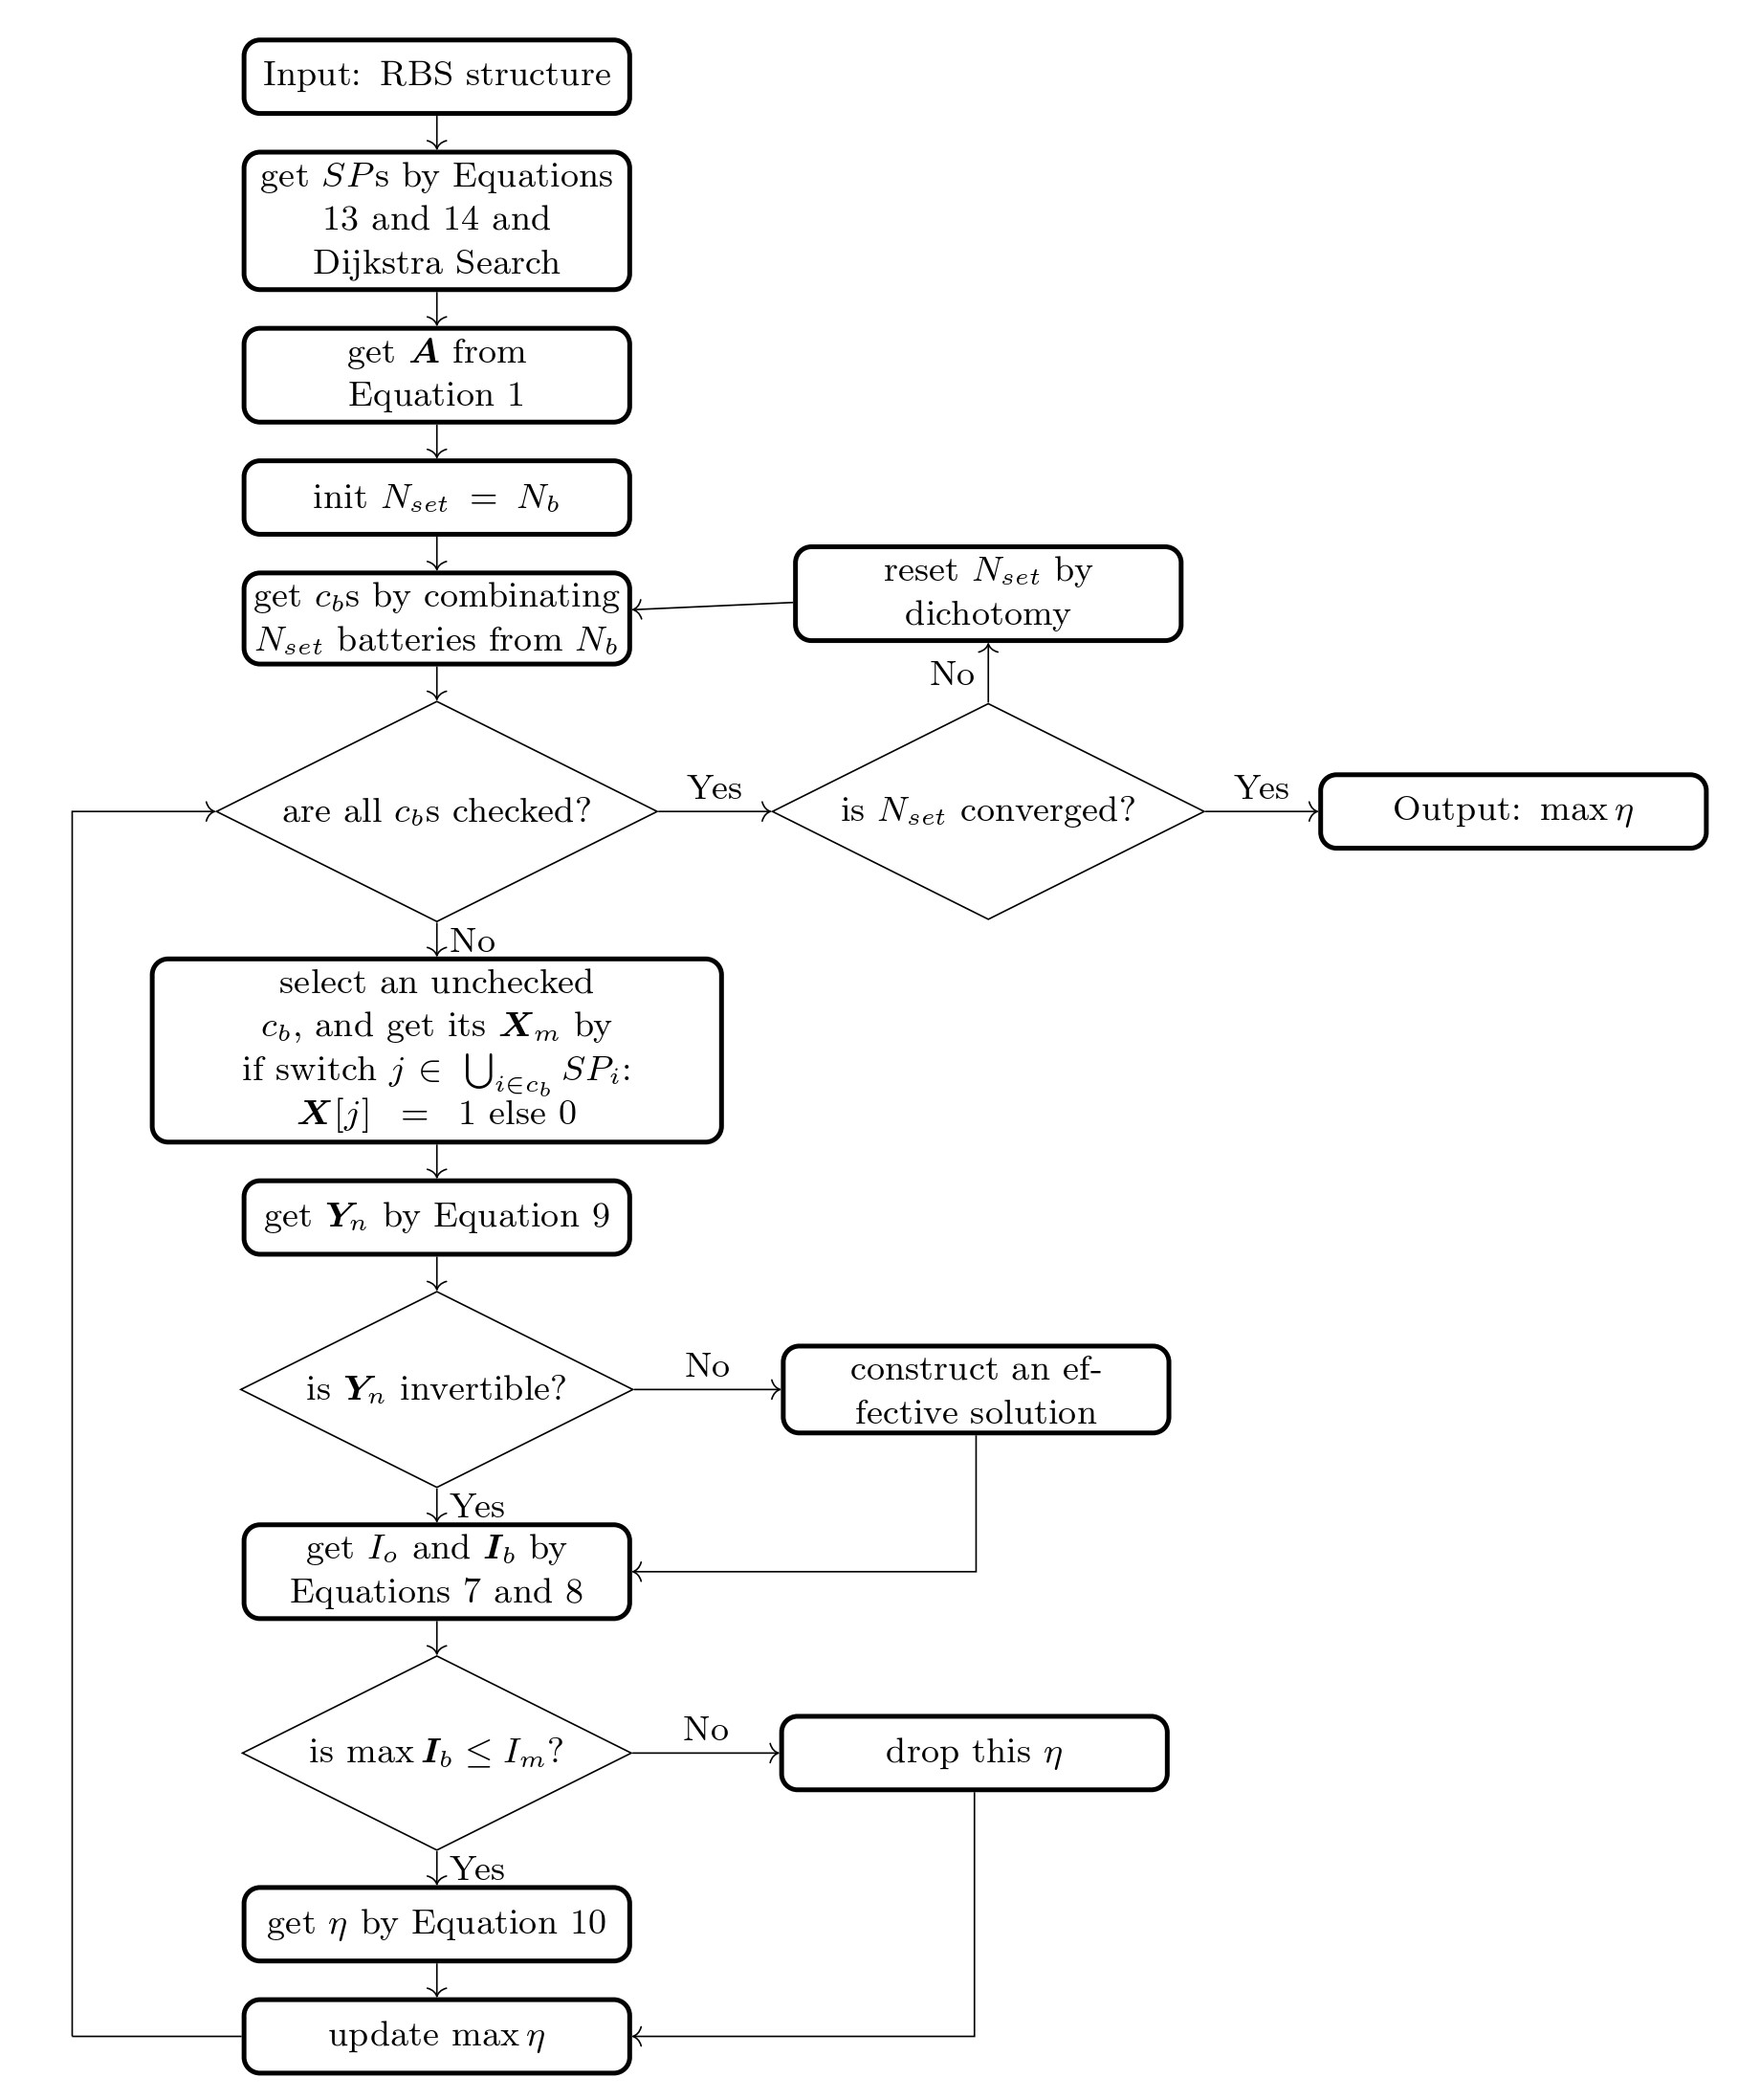
\includegraphics[width=\textwidth]{flowchart.jpg}
%DIF <      \caption{The computational flowchart of the MAC for a given RBS.}\label{fig:flowchart}
%DIF >      \caption{Computational flowchart of MAC for a given RBS.}\label{fig:flowchart}
% \end{figure}

\section{Case Study}

\subsection{Structures}

\begin{figure}[htbp]
    \centering
    \begin{subfigure}[b]{0.2\textwidth}
        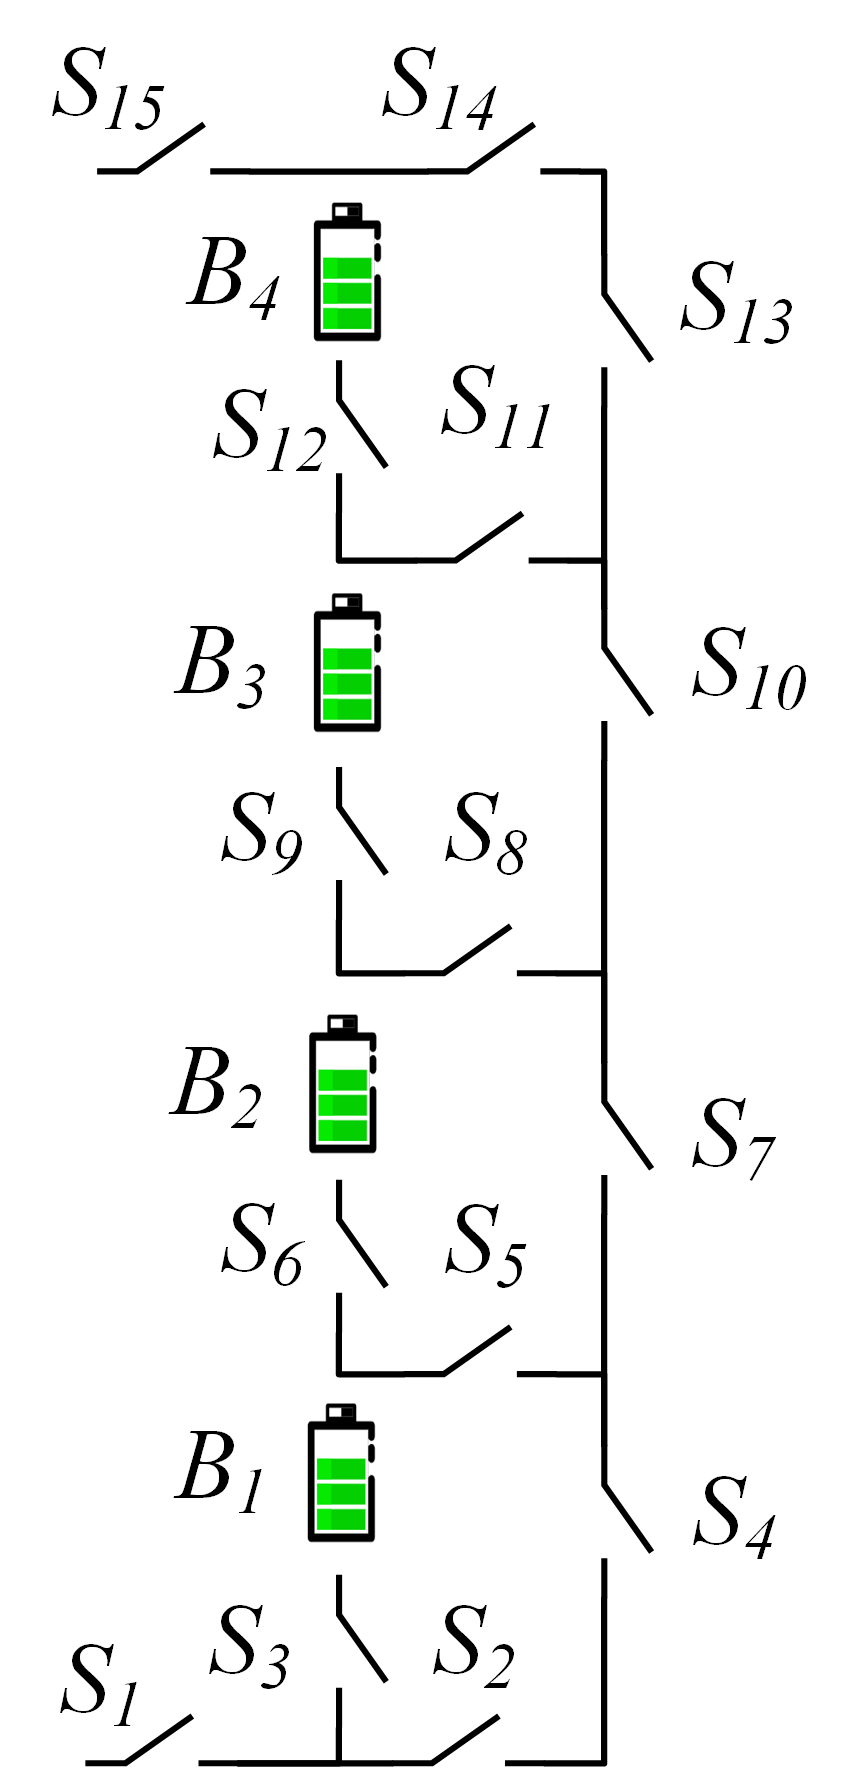
\includegraphics[width=\textwidth]{stru-L-origin.png}
        \caption{}
        \label{fig:study-stru-Lawson}
    \end{subfigure}
    \hspace{0.02\textwidth}
    \begin{subfigure}[b]{0.4\textwidth}
        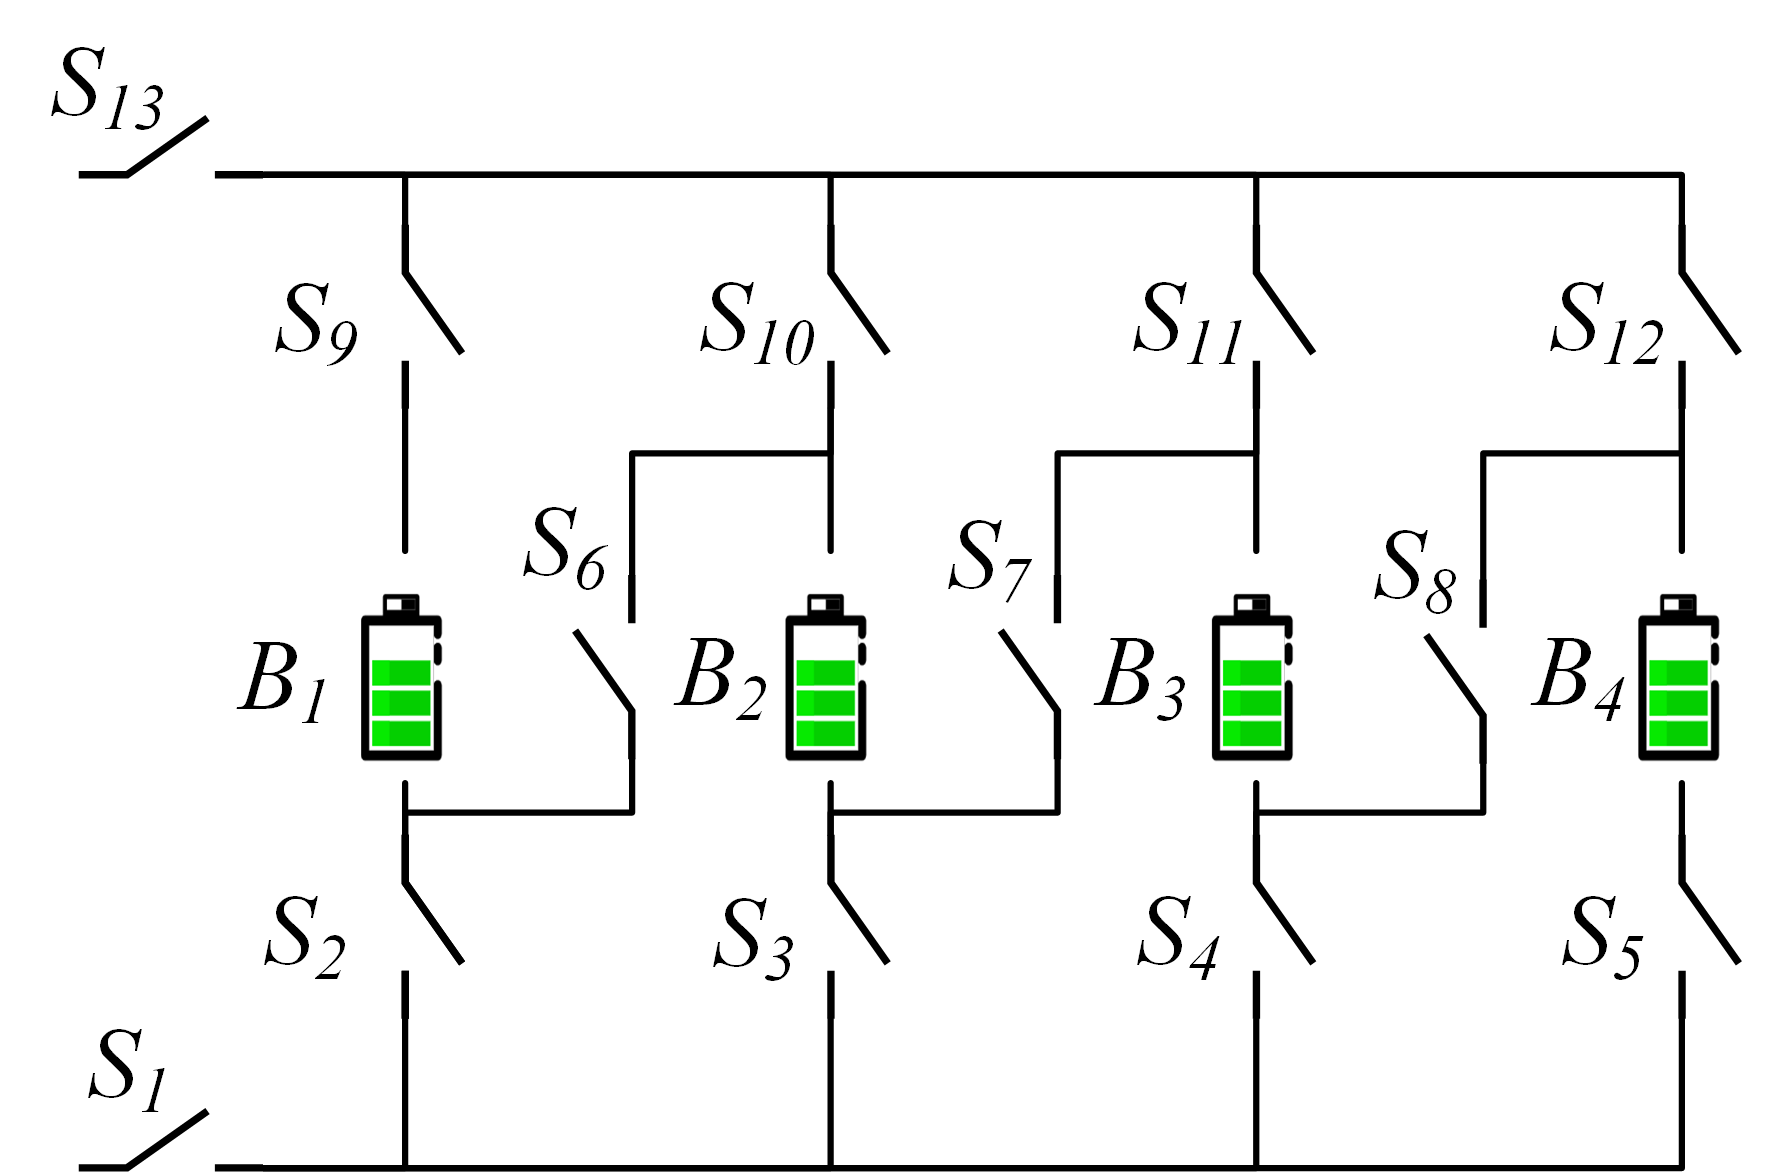
\includegraphics[width=\textwidth]{stru-V-origin.png}
        \caption{}
        \label{fig:study-stru-Visairo}
    \end{subfigure}
    \hspace{0.02\textwidth}
    \begin{subfigure}[b]{0.31\textwidth}
        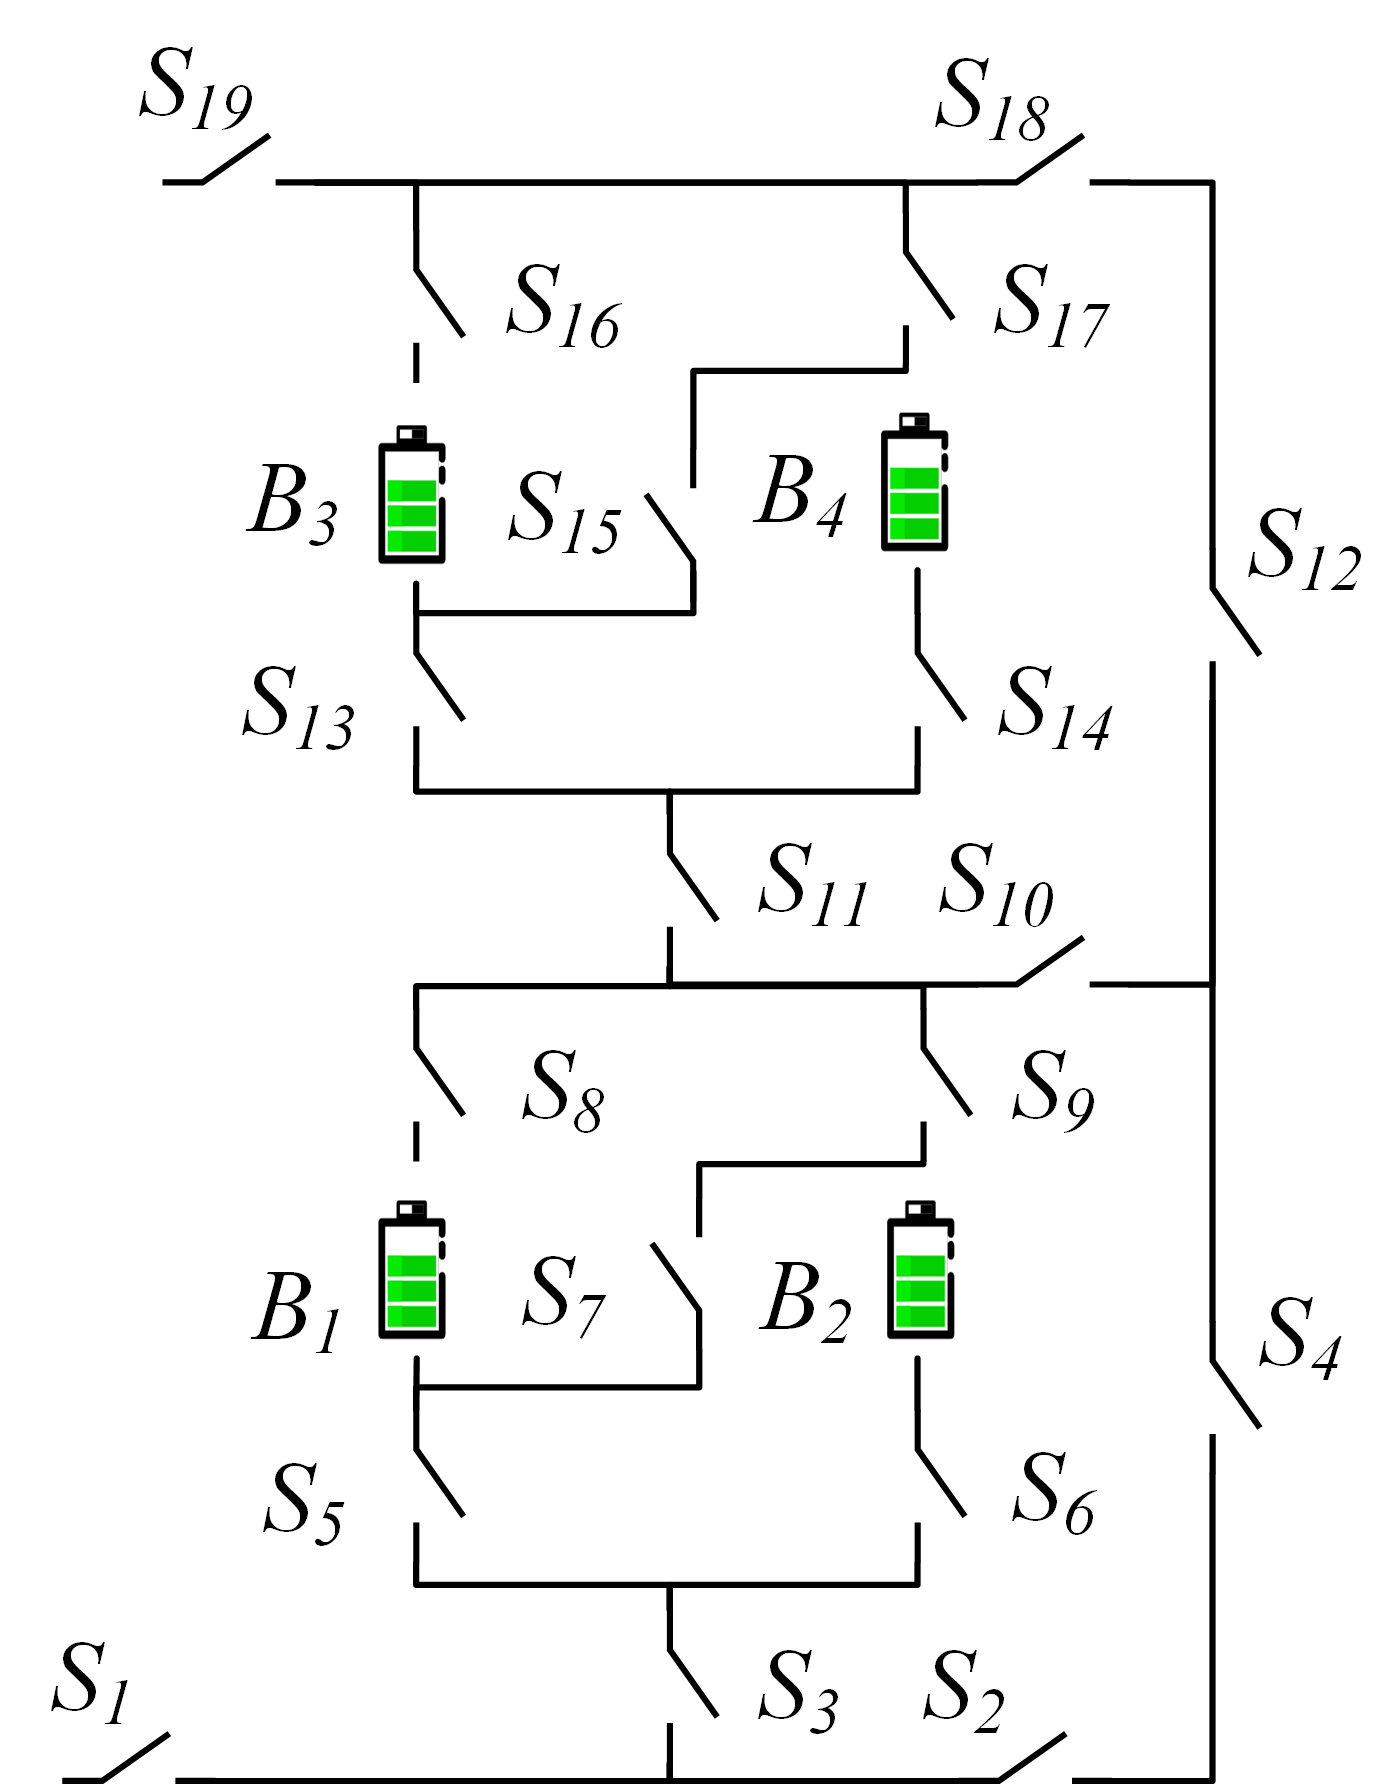
\includegraphics[width=\textwidth]{stru-my-origin.png}
        \caption{}
        \label{fig:study-stru-my}
    \end{subfigure}
    \caption{The \DIFdelbeginFL \DIFdelFL{4-battery }\DIFdelendFL \DIFaddbeginFL \DIFaddFL{four-battery }\DIFaddendFL RBS structures proposed by (a) Lawson \cite{lawsonSoftwareConfigurableBattery2012}, (b) Visairo \cite{visairoReconfigurableBatteryPack2008}\DIFaddbeginFL \DIFaddFL{, }\DIFaddendFL and (c) this paper.}
\end{figure}

Currently, two types of RBS structures have been proposed by Visairo et al. \cite{visairoReconfigurableBatteryPack2008} and Lawson et al. \cite{lawsonSoftwareConfigurableBattery2012}, both of which have \DIFdelbegin \DIFdel{been }%DIFDELCMD < \replaced{practically used}{applied in practice}%%%
\DIFdelend \DIFaddbegin \DIFadd{seen real use}\DIFaddend . 
The primary goal of Visairo's structure (\DIFdelbegin \DIFdel{Figure \ref{fig:study-stru-Visairo}) was to achieve dynamic adjustment of RBS output }%DIFDELCMD < \added{power}%%%
\DIFdel{; however}\DIFdelend \DIFaddbegin \DIFadd{Fig. \ref{fig:study-stru-Visairo}) is to dynamically adjust the RBS output power. However}\DIFaddend , the isolation of unhealthy batteries \DIFdelbegin \DIFdel{was }\DIFdelend \DIFaddbegin \DIFadd{is }\DIFaddend not sufficiently addressed \DIFdelbegin %DIFDELCMD < \added{in their work}%%%
\DIFdel{. 
}%DIFDELCMD < \deleted{When batteries need to be isolated in the RBS of Visairo's structure, the methods for isolating them and the subsequent changes in RBS output warrant further investigation.}
%DIFDELCMD < %%%
\DIFdelend \DIFaddbegin \DIFadd{in their work. 
}\DIFaddend Lawson et al. \DIFdelbegin %DIFDELCMD < \replaced{designed the RBS structure shown in Figure \ref{fig:study-stru-Lawson} for the purpose of battery isolation}{conducted research on battery isolation in RBS and specifically designed the structure shown in Figure \ref{fig:study-stru-Lawson}}%%%
\DIFdel{. This structure has the advantage of easily isolating batteries, but }\DIFdelend \DIFaddbegin \DIFadd{designed the RBS structure shown in Fig. \ref{fig:study-stru-Lawson} to isolate batteries. 
Although this structure easily isolates batteries, }\DIFaddend it cannot dynamically adjust the output current of \DIFaddbegin \DIFadd{the }\DIFaddend RBS. 
Based on the structures of Visairo and Lawson, this paper \DIFdelbegin \DIFdel{presents a new structure , as shown in Figure \ref{fig:study-stru-my}}%DIFDELCMD < \deleted{, which combines the advantages of both}%%%
\DIFdelend \DIFaddbegin \DIFadd{proposes the structure shown in Fig. \ref{fig:study-stru-my}}\DIFaddend .
By integrating the Visairo RBS structure into the Lawson RBS structure, the \DIFdelbegin \DIFdel{new }\DIFdelend \DIFaddbegin \DIFadd{proposed }\DIFaddend structure not only \DIFdelbegin \DIFdel{allows }\DIFdelend \DIFaddbegin \DIFadd{has }\DIFaddend the flexibility to switch the batteries between series, parallel, and mixed series-parallel modes \DIFdelbegin \DIFdel{, but also easily enables }\DIFdelend \DIFaddbegin \DIFadd{but also allows }\DIFaddend the isolation of highly degraded batteries from the RBS.
\DIFdelbegin \DIFdel{And their variations }\DIFdelend \DIFaddbegin \DIFadd{Their variation }\DIFaddend in output current under battery isolation \DIFdelbegin \DIFdel{conditions }\DIFdelend will be studied.
This RBS structure \DIFdelbegin \DIFdel{will be }\DIFdelend \DIFaddbegin \DIFadd{is }\DIFaddend used to validate the \DIFdelbegin \DIFdel{effectiveness of the }\DIFdelend proposed method for calculating the MAC \DIFdelbegin \DIFdel{, and be compared with the }\DIFdelend \DIFaddbegin \DIFadd{and is compared with }\DIFaddend Lawson's and Visairo's structure to \DIFdelbegin \DIFdel{illustrate its advantage on }\DIFdelend \DIFaddbegin \DIFadd{demonstrate its advantages for }\DIFaddend battery isolation.

\subsection{Result}

As shown in \DIFdelbegin \DIFdel{Figure }\DIFdelend \DIFaddbegin \DIFadd{Fig. }\DIFaddend \ref{fig:study-stru-my}, the new RBS structure consists of \DIFdelbegin \DIFdel{4 }\DIFdelend \DIFaddbegin \DIFadd{four }\DIFaddend batteries and 19 switches. 
\DIFdelbegin \DIFdel{The }\DIFdelend \DIFaddbegin \DIFadd{Figure \ref{fig:study-dirgraph-my} shows the }\DIFaddend corresponding directed graph\DIFdelbegin \DIFdel{is depicted in Figure \ref{fig:study-dirgraph-my}}\DIFdelend , which is composed of \DIFdelbegin \DIFdel{a total of }\DIFdelend 18 nodes and 43 edges. 
Batteries $B_1$, $B_2$, $B_3$, and $B_4$ are denoted by green directed edges in the graph, \DIFdelbegin \DIFdel{while }\DIFdelend \DIFaddbegin \DIFadd{and }\DIFaddend the 19 switches are represented by gray directed edges with \DIFdelbegin \DIFdel{bi-directional }\DIFdelend \DIFaddbegin \DIFadd{bidirectional }\DIFaddend arrows. 
The external electrical load is treated as a directed edge from the cathode of the RBS (i.e., node 18) to the anode (i.e., node 1), as indicated by the blue directed edge in the graph.
\DIFdelbegin \DIFdel{Utilizing Equation \ref{eq:weight}}\DIFdelend \DIFaddbegin \DIFadd{Using Eq. (\ref{eq:weight}) }\DIFaddend and the Dijkstra algorithm, the $SP$s of the four batteries in the RBS structure of \DIFdelbegin \DIFdel{Figure }\DIFdelend \DIFaddbegin \DIFadd{Fig. }\DIFaddend \ref{fig:study-stru-my} are highlighted \DIFdelbegin \DIFdel{by red in Figures \ref{fig:sp1} -}\DIFdelend \DIFaddbegin \DIFadd{in red in Figs. \ref{fig:sp1} and }\DIFaddend \ref{fig:sp4}.
Finally, the \DIFdelbegin \DIFdel{MAC calculation results }\DIFdelend \DIFaddbegin \DIFadd{calculated MACs }\DIFaddend of the structure in \DIFdelbegin \DIFdel{Figure \ref{fig:study-stru-my} are shown as }\DIFdelend \DIFaddbegin \DIFadd{Fig. \ref{fig:study-stru-my} are listed in }\DIFaddend Table \ref{tab:study-results-my} and \DIFdelbegin \DIFdel{Figure \ref{fig:study-results-my}, }\DIFdelend \DIFaddbegin \DIFadd{Fig. \ref{fig:study-results-my}, as }\DIFaddend obtained by the greedy algorithm \ref{alg:greedy}.
Table \ref{tab:study-results-my} contains the \DIFdelbegin \DIFdel{switches states }\DIFdelend \DIFaddbegin \DIFadd{states of the switches}\DIFaddend , the output current $I_o$, \DIFaddbegin \DIFadd{the }\DIFaddend battery current $\bm{I}_b$\DIFdelbegin \DIFdel{and }\DIFdelend \DIFaddbegin \DIFadd{, and the }\DIFaddend ratio $\eta$ of the RBS structure with all batteries in good health when the RBS output reaches the MAC.
Figure \ref{fig:study-results-my} presents the corresponding circuit, with the red highlight indicating that \DIFaddbegin \DIFadd{the }\DIFaddend current is flowing through the respective branches.

\begin{figure}[htbp]
    \centering
    \begin{subfigure}[b]{0.28\textwidth}
        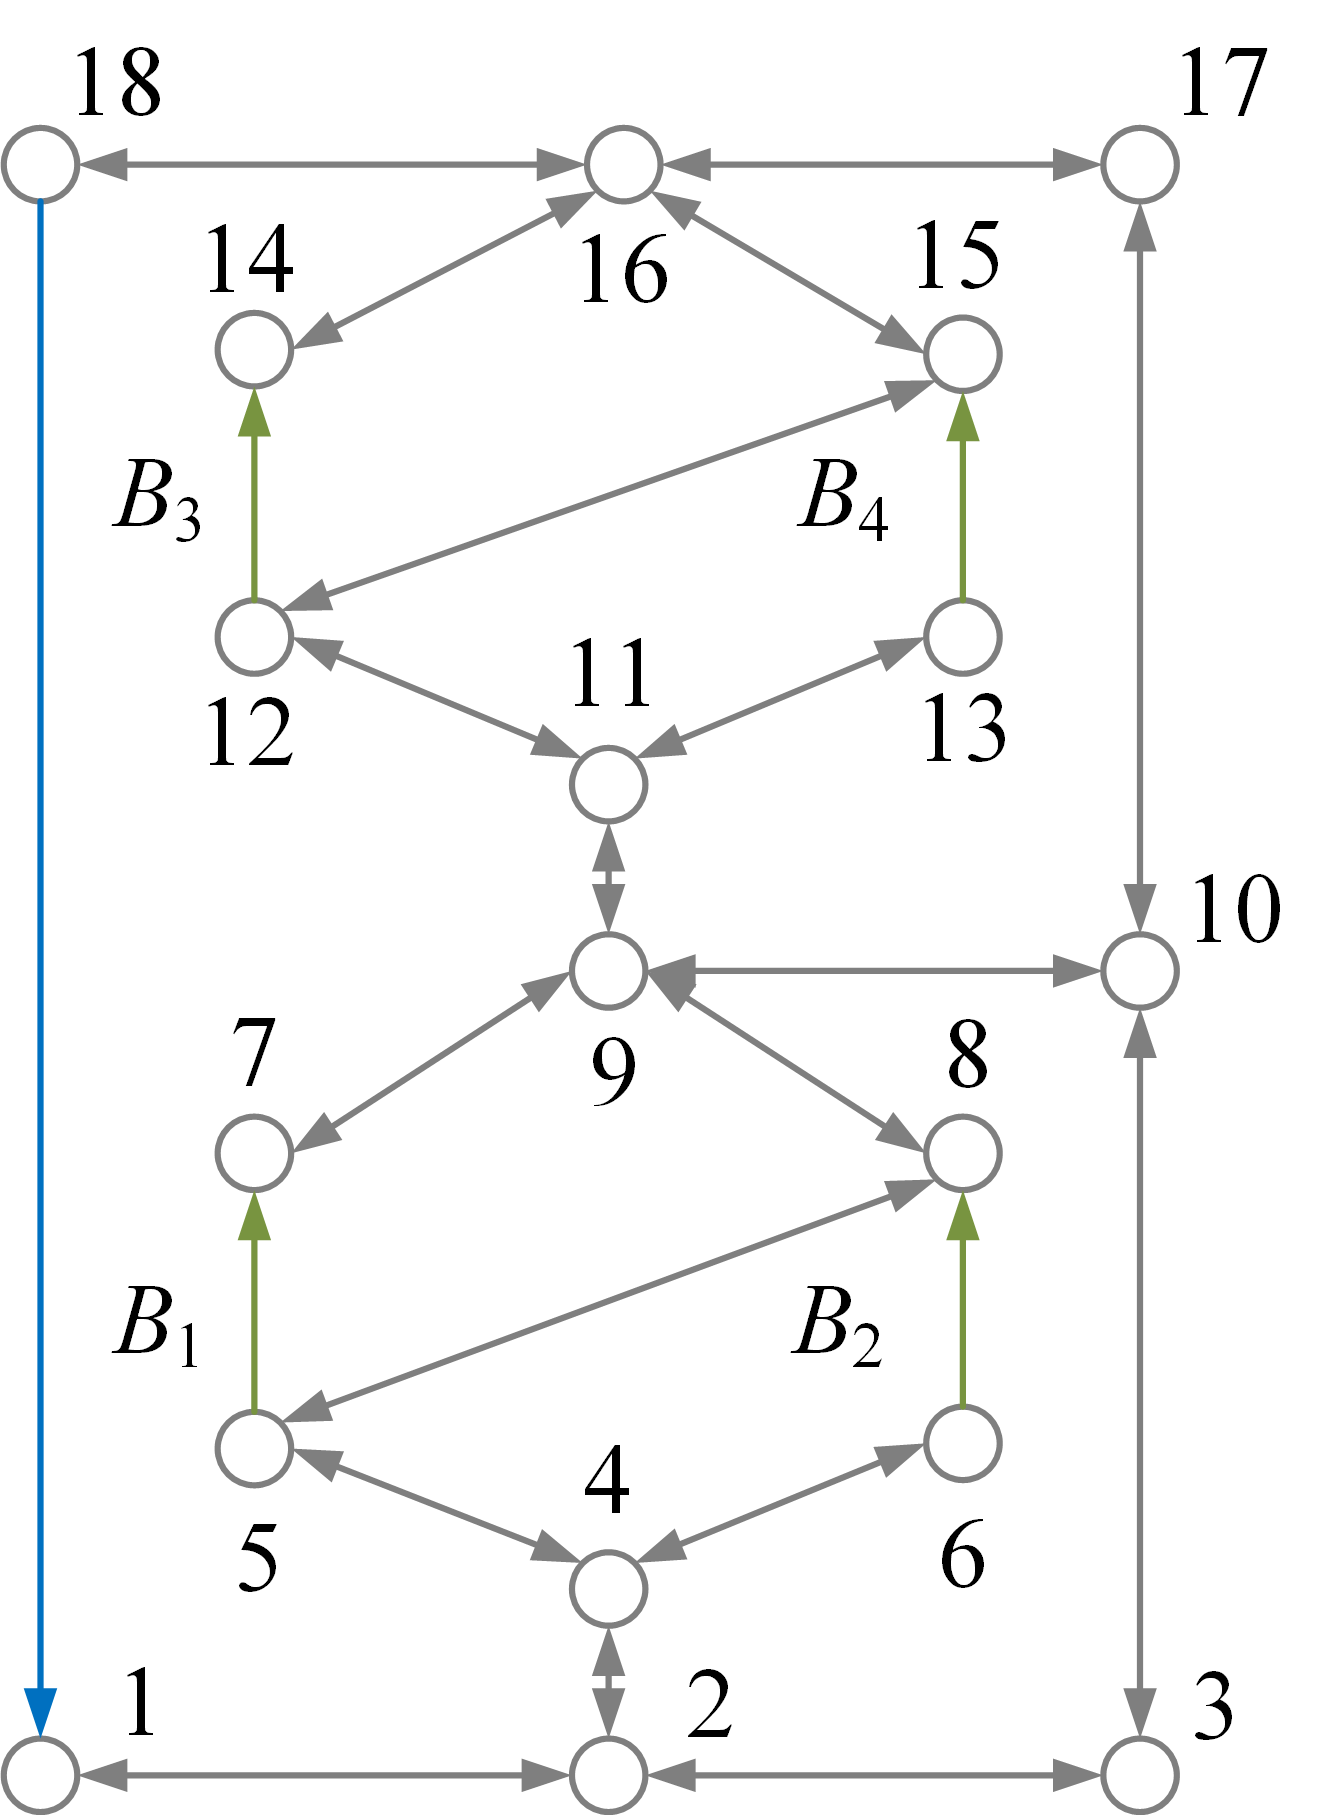
\includegraphics[width=\textwidth]{ef-topo.png}
        \caption{}
        \label{fig:study-dirgraph-my}
    \end{subfigure}
    \hspace{0.05\textwidth}
    \begin{subfigure}[b]{0.28\textwidth}
        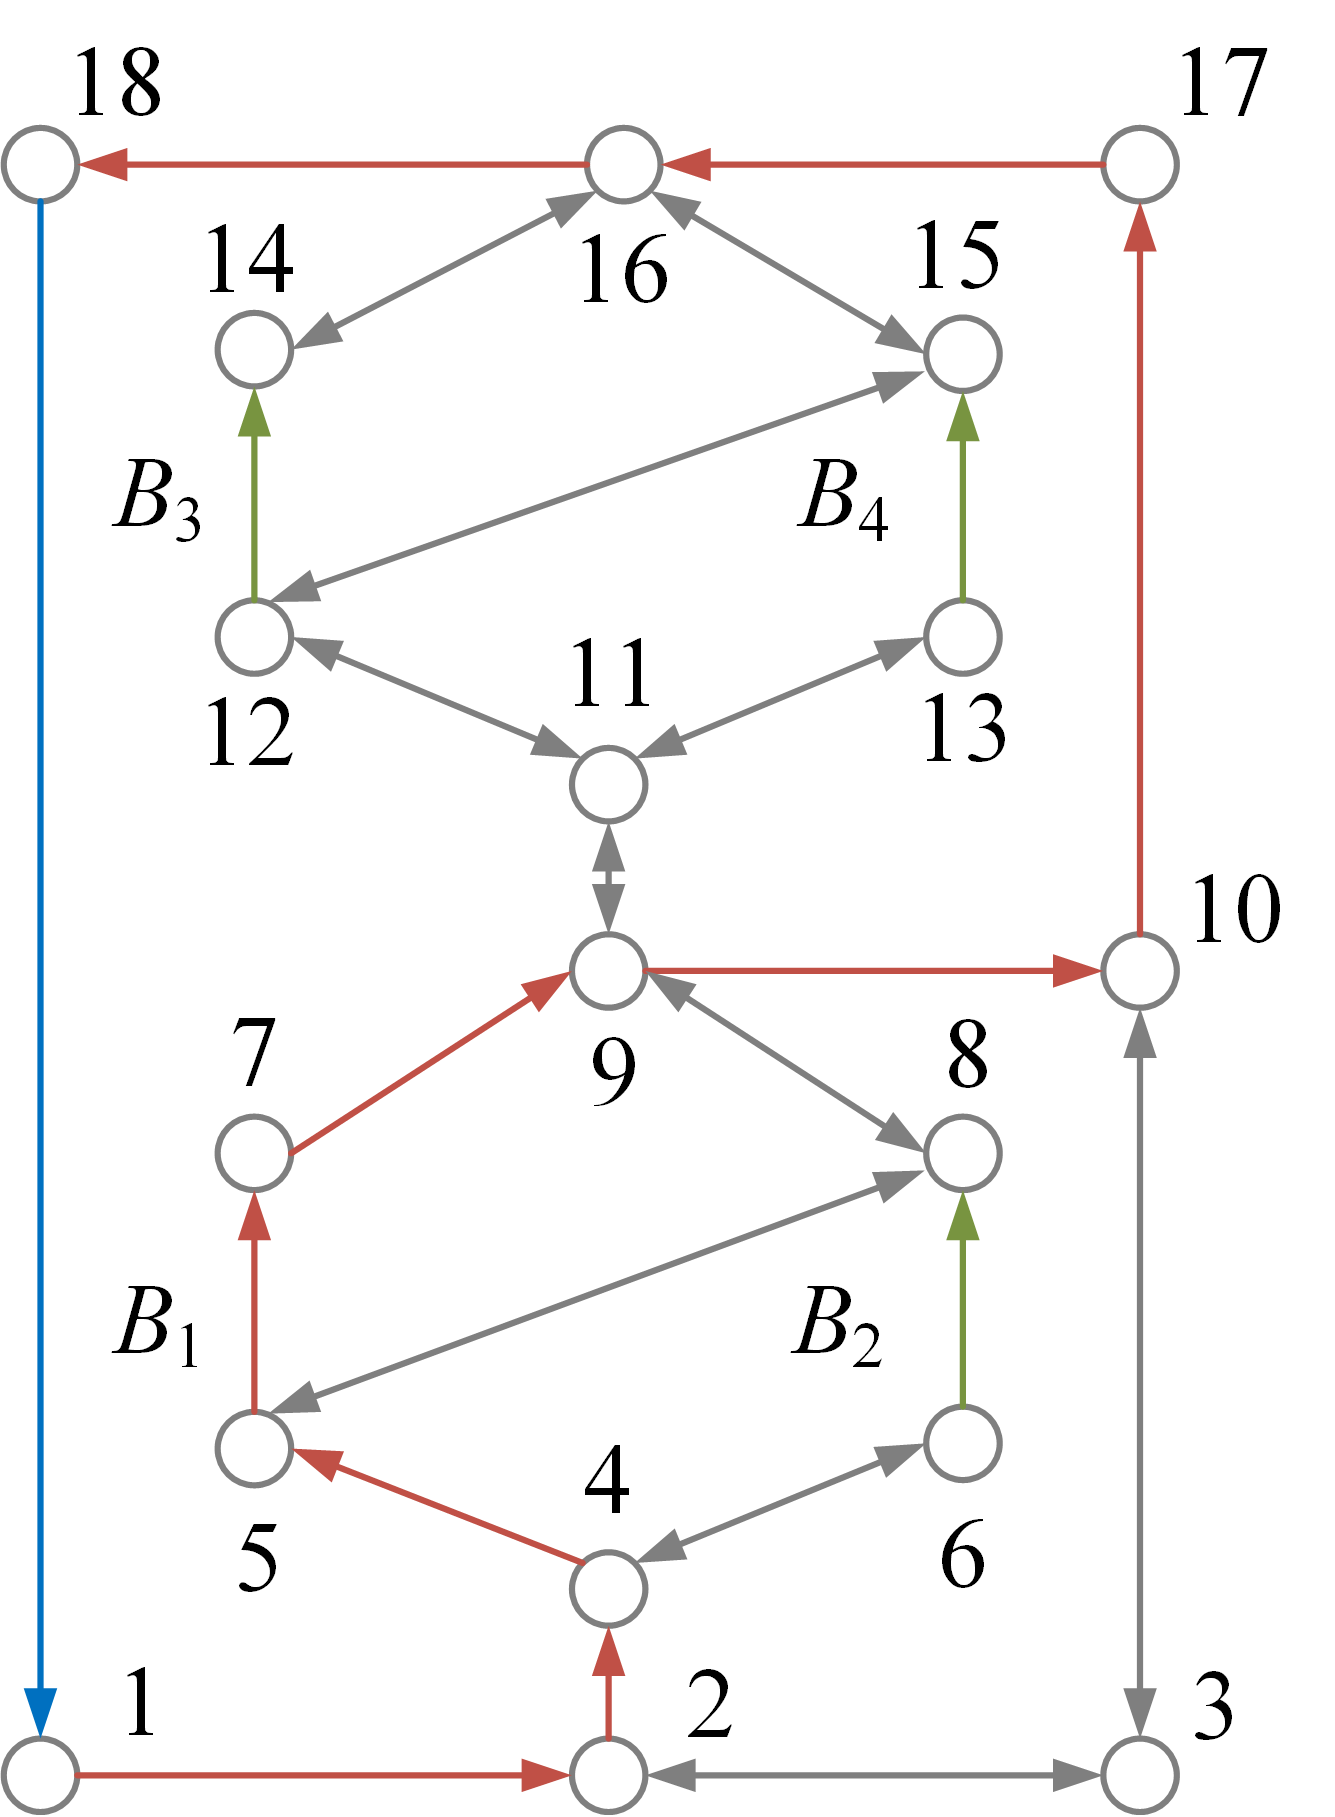
\includegraphics[width=\textwidth]{ef-sp1.png}
        \caption{}
        \label{fig:sp1}
    \end{subfigure}
    \hspace{0.05\textwidth}
    \begin{subfigure}[b]{0.28\textwidth}
        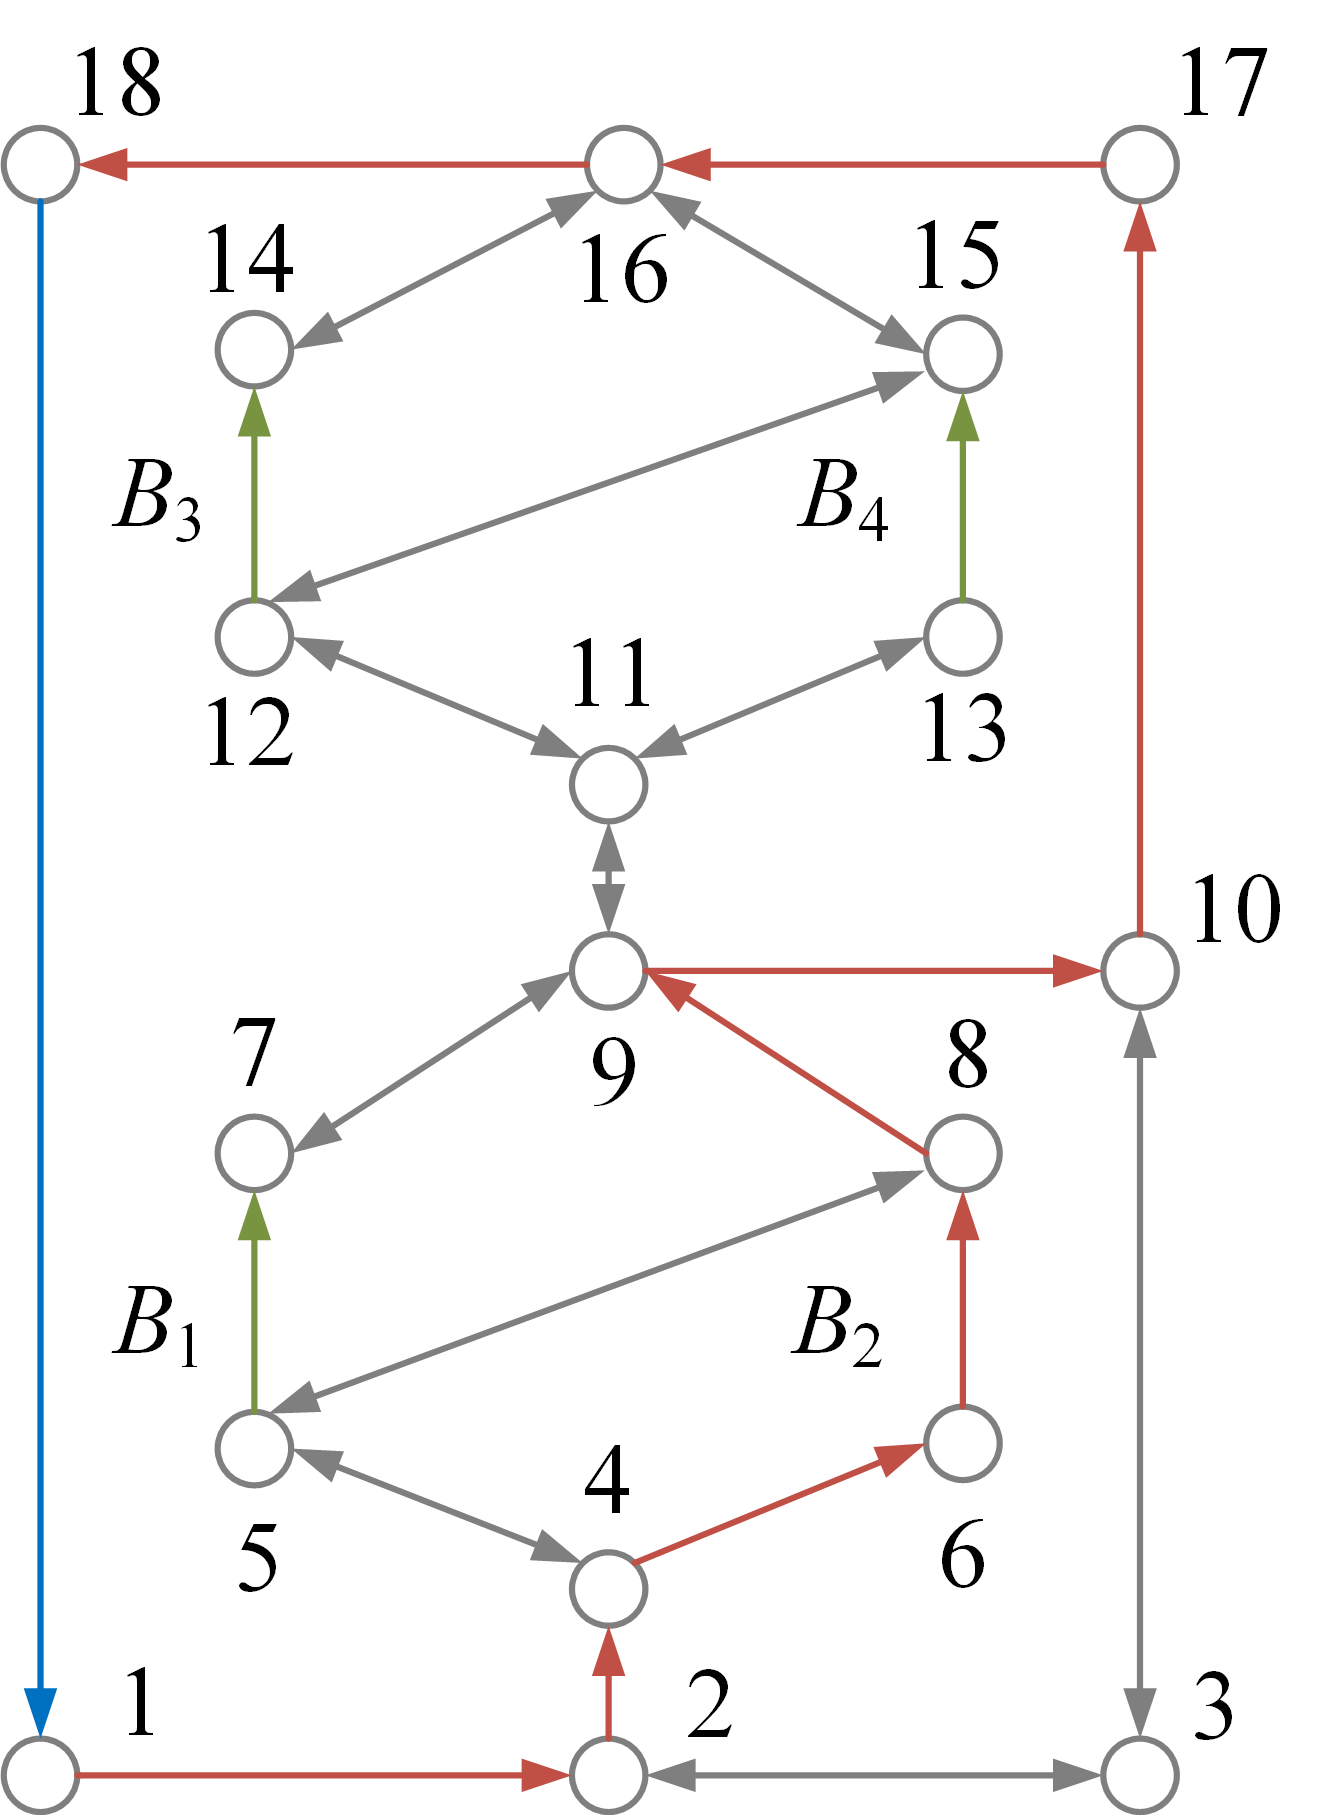
\includegraphics[width=\textwidth]{ef-sp2.png}
        \caption{}
        \label{fig:sp2}
    \end{subfigure}
    \\
    \begin{subfigure}[b]{0.28\textwidth}
        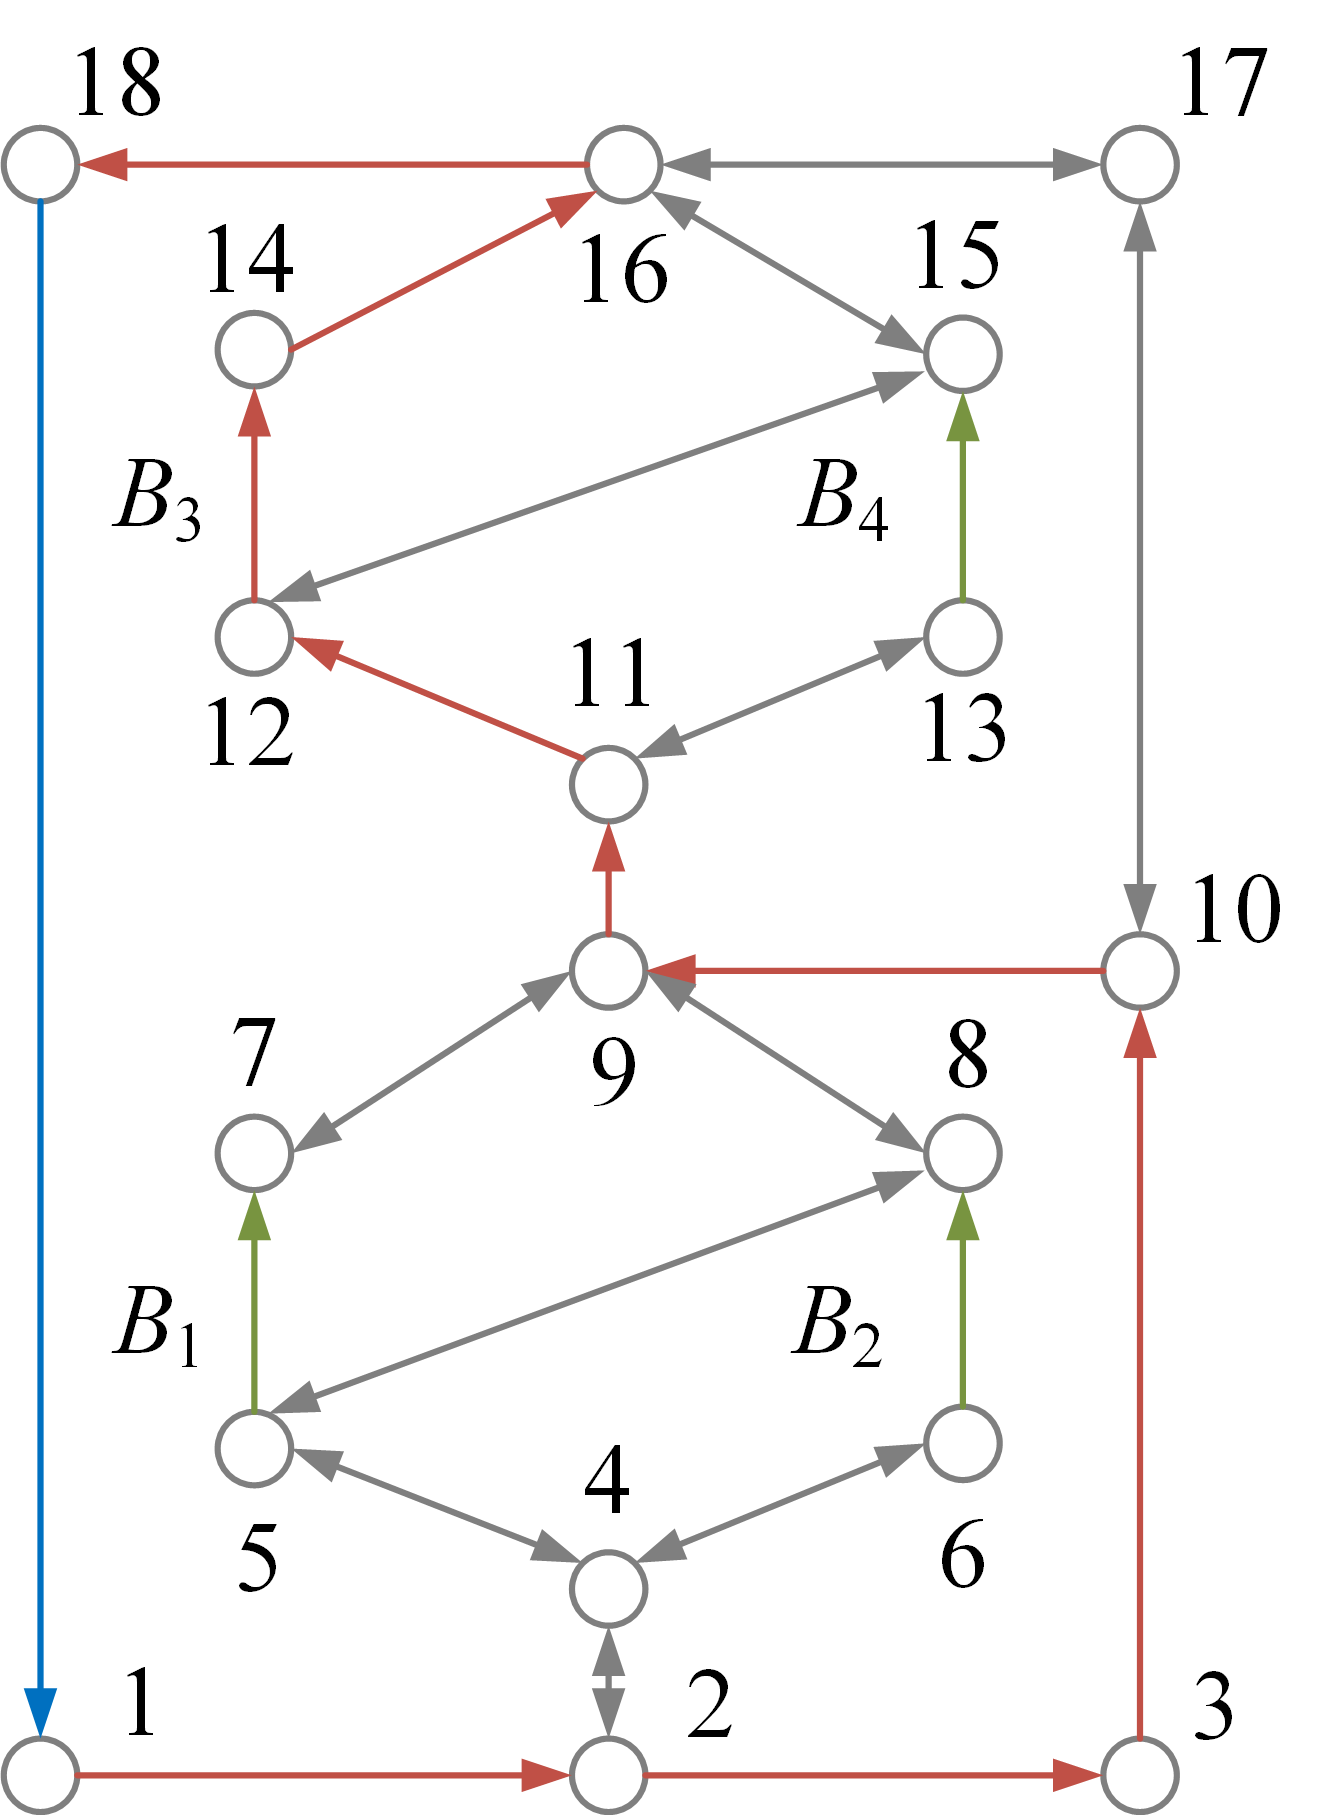
\includegraphics[width=\textwidth]{ef-sp3.png}
        \caption{}
        \label{fig:sp3}
    \end{subfigure}
    \hspace{0.05\textwidth}
    \begin{subfigure}[b]{0.28\textwidth}
        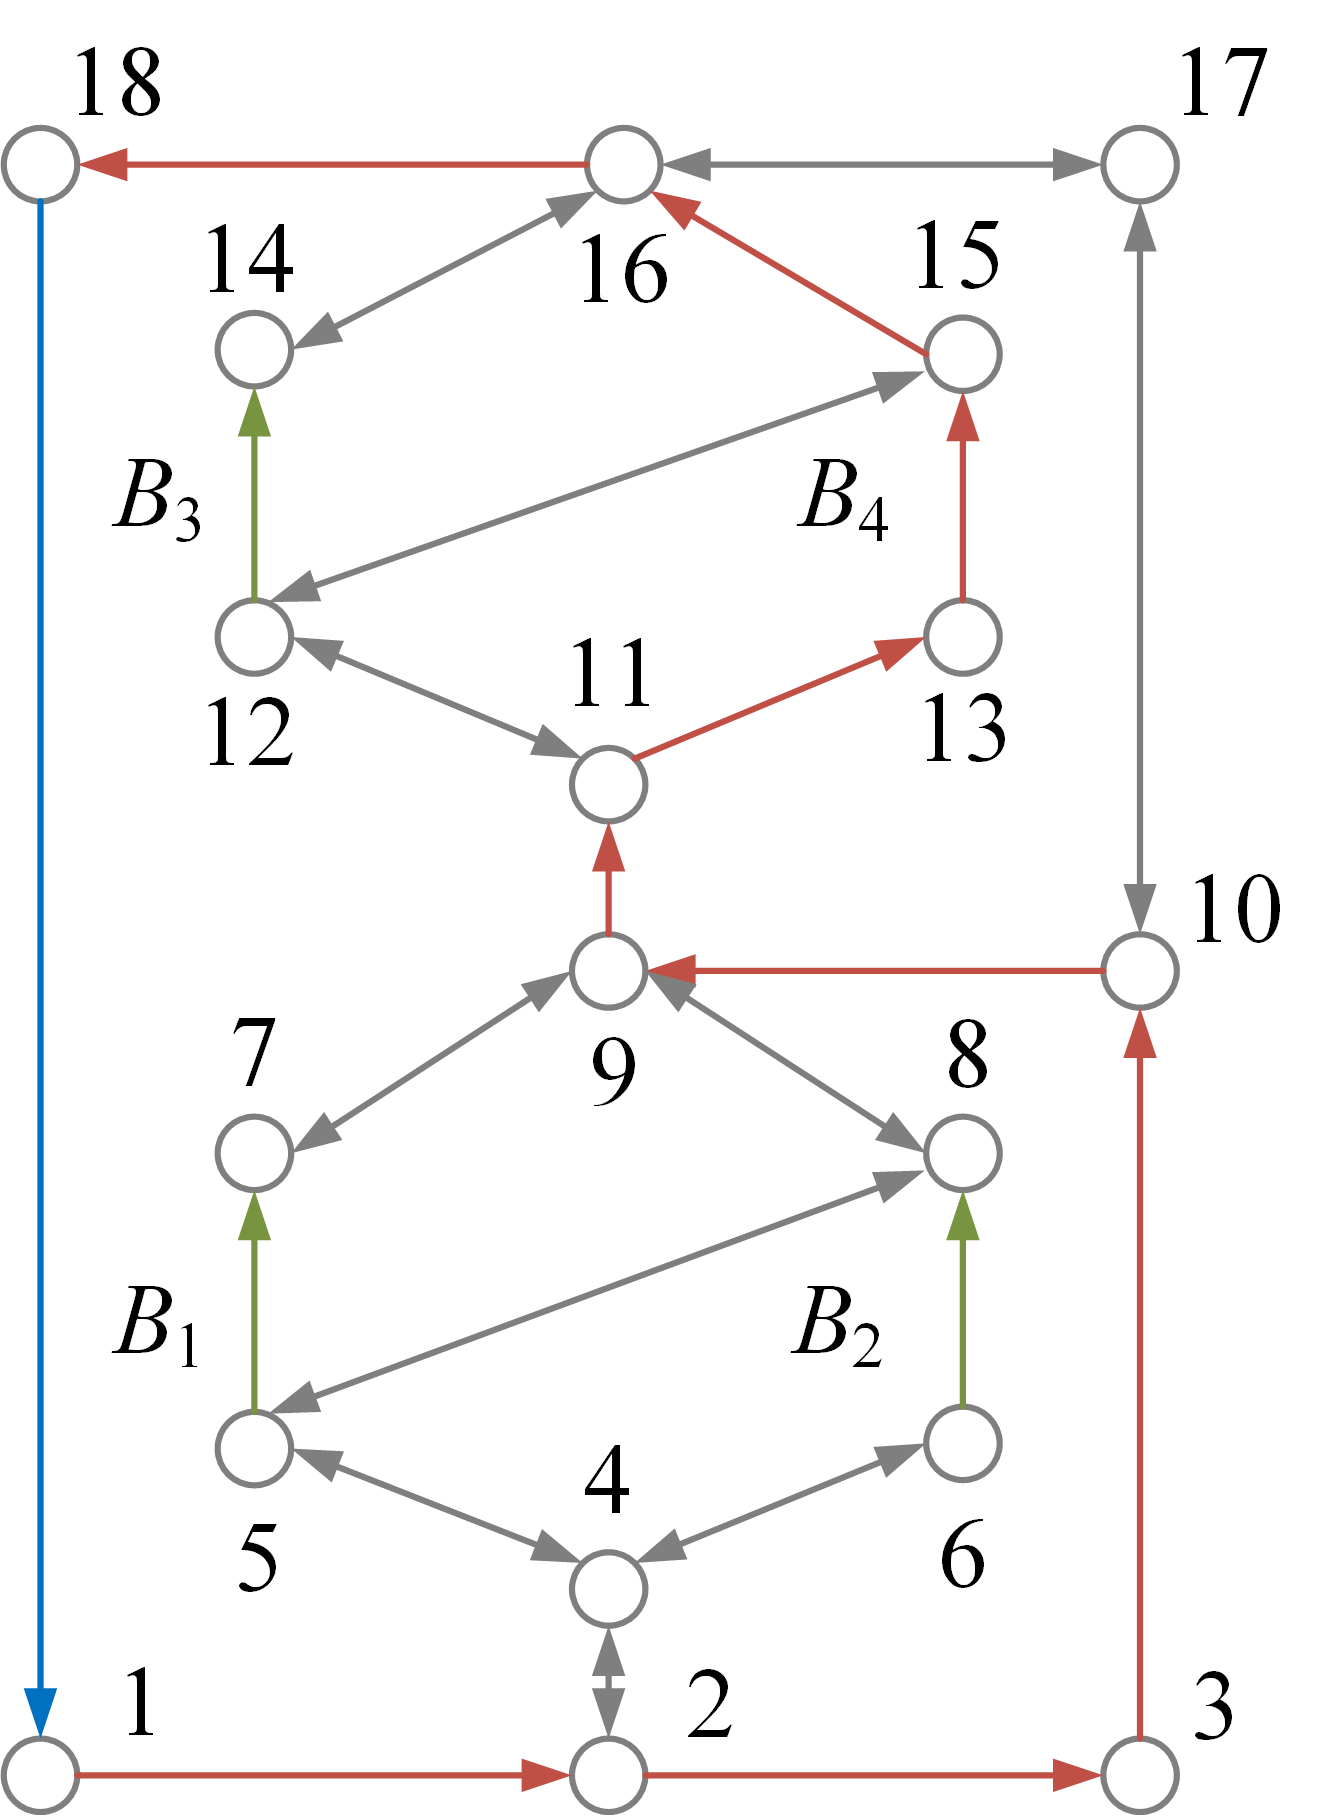
\includegraphics[width=\textwidth]{ef-sp4.png}
        \caption{}
        \label{fig:sp4}
    \end{subfigure}
    \hspace{0.05\textwidth}
    \begin{subfigure}[b]{0.28\textwidth}
        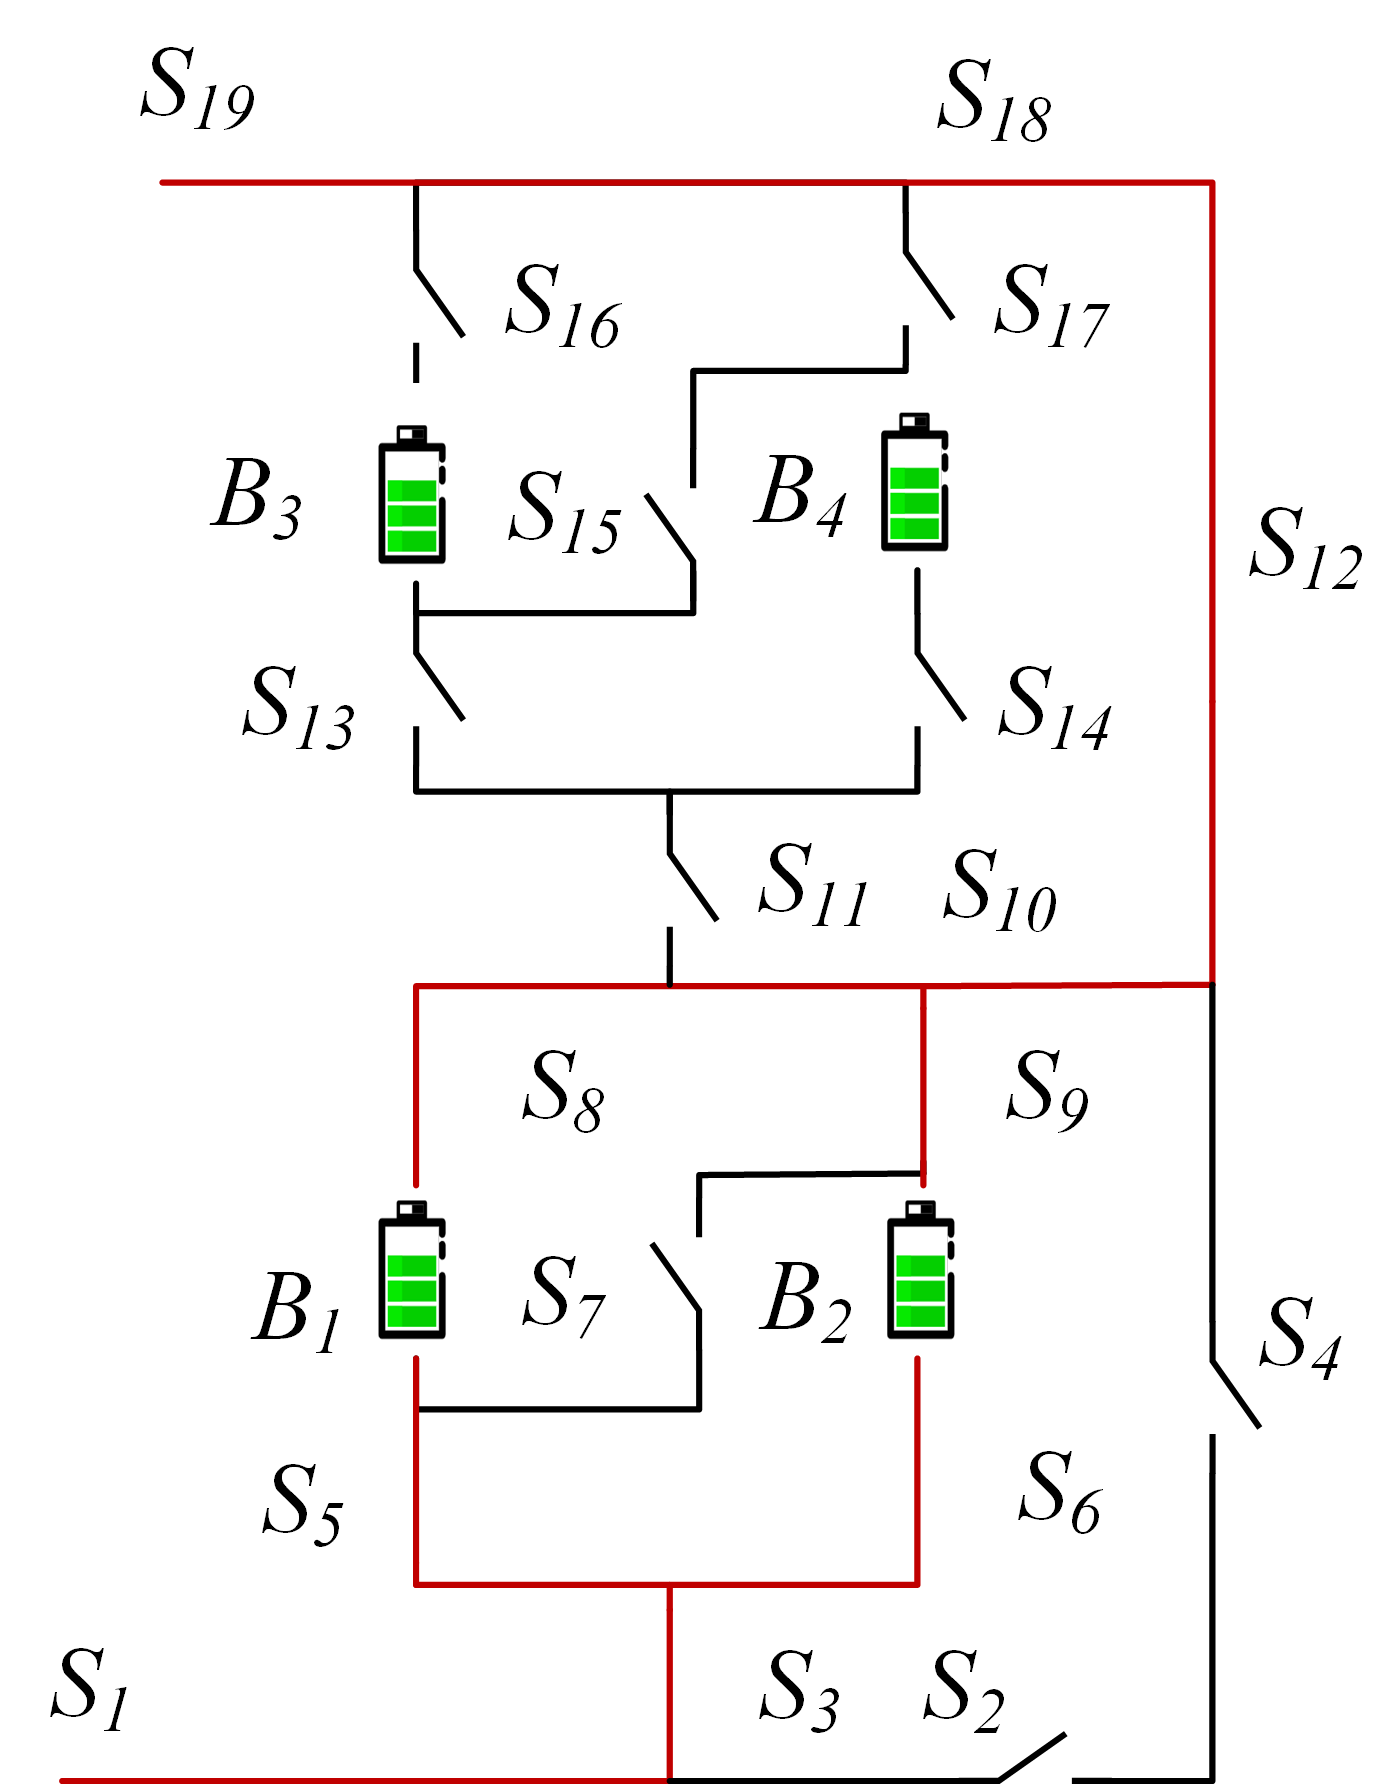
\includegraphics[width=\textwidth]{ef-mac.png}
        \caption{}
        \label{fig:study-results-my}
    \end{subfigure}
    \caption{
        For the RBS structure in \DIFdelbeginFL \DIFdelFL{Figure }\DIFdelendFL \DIFaddbeginFL \DIFaddFL{Fig. }\DIFaddendFL \ref{fig:study-stru-my}, 
        (a) its directed graph 
        and the $SP$s (highlighted in red) of battery (b) $B_1$, (c) $B_2$, (d) $B_3$, \DIFaddbeginFL \DIFaddFL{and }\DIFaddendFL (e) $B_4$.
        (f) \DIFdelbeginFL \DIFdelFL{The circuit }\DIFdelendFL \DIFaddbeginFL \DIFaddFL{Circuit }\DIFaddendFL of \DIFdelbeginFL \DIFdelFL{the }\DIFdelendFL RBS with its output reaching the MAC.
        }
    \label{fig:all-results-my}
\end{figure}

\begin{table}[htbp]
  \centering
    \caption{\DIFaddbeginFL \DIFaddFL{Calculated }\DIFaddendFL MAC \DIFdelbeginFL \DIFdelFL{Calculating result of the 4-battery }\DIFdelendFL \DIFaddbeginFL \DIFaddFL{for four-battery }\DIFaddendFL RBS structure in \DIFdelbeginFL \DIFdelFL{Figure }\DIFdelendFL \DIFaddbeginFL \DIFaddFL{Fig. }\DIFaddendFL \ref{fig:study-stru-my}.}
    \begin{tabular}{cc}
    \toprule
        Structure & Figure \ref{fig:study-stru-my} with \DIFdelbeginFL \DIFdelFL{4 }\DIFdelendFL \DIFaddbeginFL \DIFaddFL{four }\DIFaddendFL batteries and 19 switches  \\
    \midrule
    Switch \DIFdelbeginFL \DIFdelFL{ON }\DIFdelendFL \DIFaddbeginFL \DIFaddFL{on }\DIFaddendFL & $S_1$,$S_3$,$S_5$,$S_6$,$S_8$,$S_9$,$S_{10}$,$S_{12}$,$S_{18}$,$S_{19}$ \\
    $I_o$ & $2u_b/(2R_o+r_b)$ \\
    $\bm{I}_b$ & $[u_b/(2R_o+r_b),u_b/(2R_o+r_b),0,0]$ \\
    \DIFdelbeginFL %DIFDELCMD < \added{$\max$}%%%
\DIFdelFL{$\eta$     }\DIFdelendFL \DIFaddbeginFL \DIFaddFL{$\max \eta$     }\DIFaddendFL & 2 \\
    \bottomrule
    \end{tabular}
  \label{tab:study-results-my}
\end{table}

Similarly, the \DIFdelbegin \DIFdel{MAC calculation }\DIFdelend results of the \DIFdelbegin \DIFdel{structures in Figures }\DIFdelend \DIFaddbegin \DIFadd{MAC calculation for the structures in Figs. }\DIFaddend \ref{fig:study-stru-Lawson} and \ref{fig:study-stru-Visairo} are \DIFdelbegin \DIFdel{shown as Table \ref{tab:study-results-Lawson} and  Table }\DIFdelend \DIFaddbegin \DIFadd{listed in Tables \ref{tab:study-results-Lawson} and  }\DIFaddend \ref{tab:study-results-Visairo}, respectively.
\DIFdelbegin %DIFDELCMD < \added{
%DIFDELCMD < In order to verify and compare the results from the greedy algorithm, we also utilized a brute force algorithm that go through all possible switch states to calculate the MAC of the same three RBS. 
%DIFDELCMD < For a given RBS structure with $N_s$ switches, the final $\max$ $\eta$ is the maximum of $\eta$s from all $2^{N_s}$ reconfigured structures.
%DIFDELCMD < The final results are the same as the results shown in Tables \ref{tab:study-results-my}-\ref{tab:study-results-Visairo}.
%DIFDELCMD < It is worth noting that the method used the greedy algorithm only calculated 7, 11, and 1 reconfigured structures for the RBS structure in Figures \ref{fig:study-stru-my}, \ref{fig:study-stru-Lawson}, \ref{fig:study-stru-Visairo}, respectively. 
%DIFDELCMD < While for the same RBS, the method counted all possible switch states computed $2^{19}$, $2^{15}$, and $2^{13}$ structures, respectively.
%DIFDELCMD < }
%DIFDELCMD < %%%
\DIFdelend \DIFaddbegin \DIFadd{To verify and compare the results from the greedy algorithm, we also used a brute-force algorithm that iterates through all possible switch states to calculate the MAC of the same three RBSs. 
For a given RBS structure with $N_s$ switches, the final $\max \eta$ is the maximum $\eta$ from all $2^{N_s}$ reconfigured structures.
The final results are the same as the results shown in Tables \ref{tab:study-results-my}--\ref{tab:study-results-Visairo}.
The method uses the greedy algorithm to calculate 7, 11, and 1 reconfigured structures for the RBS structure in Figs. \ref{fig:study-stru-my}, \ref{fig:study-stru-Lawson}, and \ref{fig:study-stru-Visairo}, respectively. 
For the same RBS, the method counts all possible switch states, which equates to $2^{19}$, $2^{15}$, and $2^{13}$ structures, respectively.
}\DIFaddend 

\begin{table}[htbp]
  \centering
    \caption{MAC Calculating result of the 4-battery RBS structure in \DIFdelbeginFL \DIFdelFL{Figure }\DIFdelendFL \DIFaddbeginFL \DIFaddFL{Fig. }\DIFaddendFL \ref{fig:study-stru-Lawson}.}
    \begin{tabular}{cc}
    \toprule
        Structure & Figure \ref{fig:study-stru-Lawson} with 4 batteries and 15 switches  \\
    \midrule
    Switch ON & $S_1$,$S_3$,$S_5$,$S_7$,$S_{10}$,$S_{13}$,$S_{14}$,$S_{15}$ \\
    $I_o$ & $u_b/(R_o+r_b)$ \\
    $\bm{I}_b$ & $[u_b/(R_o+r_b),0,0,0]$ \\
    \DIFdelbeginFL %DIFDELCMD < \added{$\max$}%%%
\DIFdelFL{$\eta$     }\DIFdelendFL \DIFaddbeginFL \DIFaddFL{$\max \eta$     }\DIFaddendFL & 1 \\
    \bottomrule
    \end{tabular}
  \label{tab:study-results-Lawson}
\end{table}

\begin{table}[htbp]
  \centering
    \caption{MAC Calculating result of the 4-battery RBS structure in \DIFdelbeginFL \DIFdelFL{Figure }\DIFdelendFL \DIFaddbeginFL \DIFaddFL{Fig. }\DIFaddendFL \ref{fig:study-stru-Visairo}.}
    \begin{tabular}{cc}
    \toprule
        Structure & Figure \ref{fig:study-stru-Visairo} with 4 batteries and 13 switches  \\
    \midrule
    Switch ON & $S_1$,$S_2$,$S_3$,$S_4$,$S_5$,$S_9$,$S_{10}$,$S_{11}$,$S_{12}$,$S_{13}$ \\
    $I_o$ & $4u_b/(4R_o+r_b)$ \\
    $\bm{I}_b$ & $[u_b/(4R_o+r_b),u_b/(4R_o+r_b),u_b/(4R_o+r_b),u_b/(4R_o+r_b)]$ \\
    \DIFdelbeginFL %DIFDELCMD < \added{$\max$}%%%
\DIFdelFL{$\eta$     }\DIFdelendFL \DIFaddbeginFL \DIFaddFL{$\max \eta$     }\DIFaddendFL & 4 \\
    \bottomrule
    \end{tabular}
  \label{tab:study-results-Visairo}
\end{table}

Furthermore, the RBS \DIFdelbegin %DIFDELCMD < \replaced{with}{under the scenario of} %%%
\DIFdelend \DIFaddbegin \DIFadd{with }\DIFaddend isolated batteries is taken into consideration and calculated. 
The MAC calculation results for the three structures under study, with varying numbers of isolated batteries, are presented in Table \ref{tab:isolated_mac}. 
Figures \ref{fig:my-isolated-1}\DIFdelbegin \DIFdel{-}\DIFdelend \DIFaddbegin \DIFadd{--}\DIFaddend \ref{fig:my-isolated-3} illustrate the corresponding \DIFdelbegin \DIFdel{switch control }\DIFdelend \DIFaddbegin \DIFadd{switch-control }\DIFaddend schemes for the new structure proposed in this paper under different \DIFdelbegin \DIFdel{isolated battery conditions .
}%DIFDELCMD < \deleted{The characteristics of these three structures in the context of battery isolation will be discussed in the next subsection.}
%DIFDELCMD < %%%
\DIFdelend \DIFaddbegin \DIFadd{conditions of isolated batteries.
}\DIFaddend 

\begin{table}[htbp]
    \centering
    \caption{
      \DIFdelbeginFL \DIFdelFL{The variation }\DIFdelendFL \DIFaddbeginFL \DIFaddFL{Variation }\DIFaddendFL of MAC with the number of isolated batteries for different RBS structures, including the structure proposed by Lawson et al., Visairo et al., and the structure proposed in this paper.
      }
      \label{tab:isolated_mac}
      \begin{tabular}{cccc}
      \toprule
      \DIFdelbeginFL %DIFDELCMD < \multirow{2}[4]{*}{number of isolated batteries} %%%
\DIFdelendFL \DIFaddbeginFL \multirow{2}[4]{*}{Number of isolated batteries} \DIFaddendFL & \multicolumn{3}{c}{$\eta$ of RBS structure} \\
  \cmidrule{2-4}          & \DIFdelbeginFL \DIFdelFL{our  }\DIFdelendFL \DIFaddbeginFL \DIFaddFL{This paper  }\DIFaddendFL & Visairo  \DIFdelbeginFL \DIFdelFL{'s  }\DIFdelendFL & Lawson  \DIFdelbeginFL \DIFdelFL{'s  }\DIFdelendFL \\
      \midrule
      0     & 2     & 4     & 1 \\
      1     & 2     & 3     & 1 \\
      2     & 2$^{\mathrm{a}}$ or 1$^{\mathrm{b}}$ & 2     & 1 \\
      3     & 1     & 1     & 1 \\
      \bottomrule
      \end{tabular}
      \\
      \DIFdelbeginFL %DIFDELCMD < \footnotesize{$^{\mathrm{a}}$ isolate two batteries within the same substructure, as shown in Figure \ref{fig:my-isolated-2b}}%%%
\DIFdelendFL \DIFaddbeginFL \footnotesize{$^{\mathrm{a}}$ Isolate two batteries within the same substructure, as shown in Fig. \ref{fig:my-isolated-2b}.}\DIFaddendFL \\
      \DIFdelbeginFL %DIFDELCMD < \footnotesize{$^{\mathrm{b}}$ isolate one battery in each of the two substructures, as shown in Figure \ref{fig:my-isolated-2w}}
%DIFDELCMD <   %%%
\DIFdelendFL \DIFaddbeginFL \footnotesize{$^{\mathrm{b}}$ Isolate one battery in each of the two substructures, as shown in Fig. \ref{fig:my-isolated-2w}.}
  \DIFaddendFL \end{table}

  
  \begin{figure}[htbp]
      \centering
      \begin{subfigure}[b]{0.31\textwidth}
          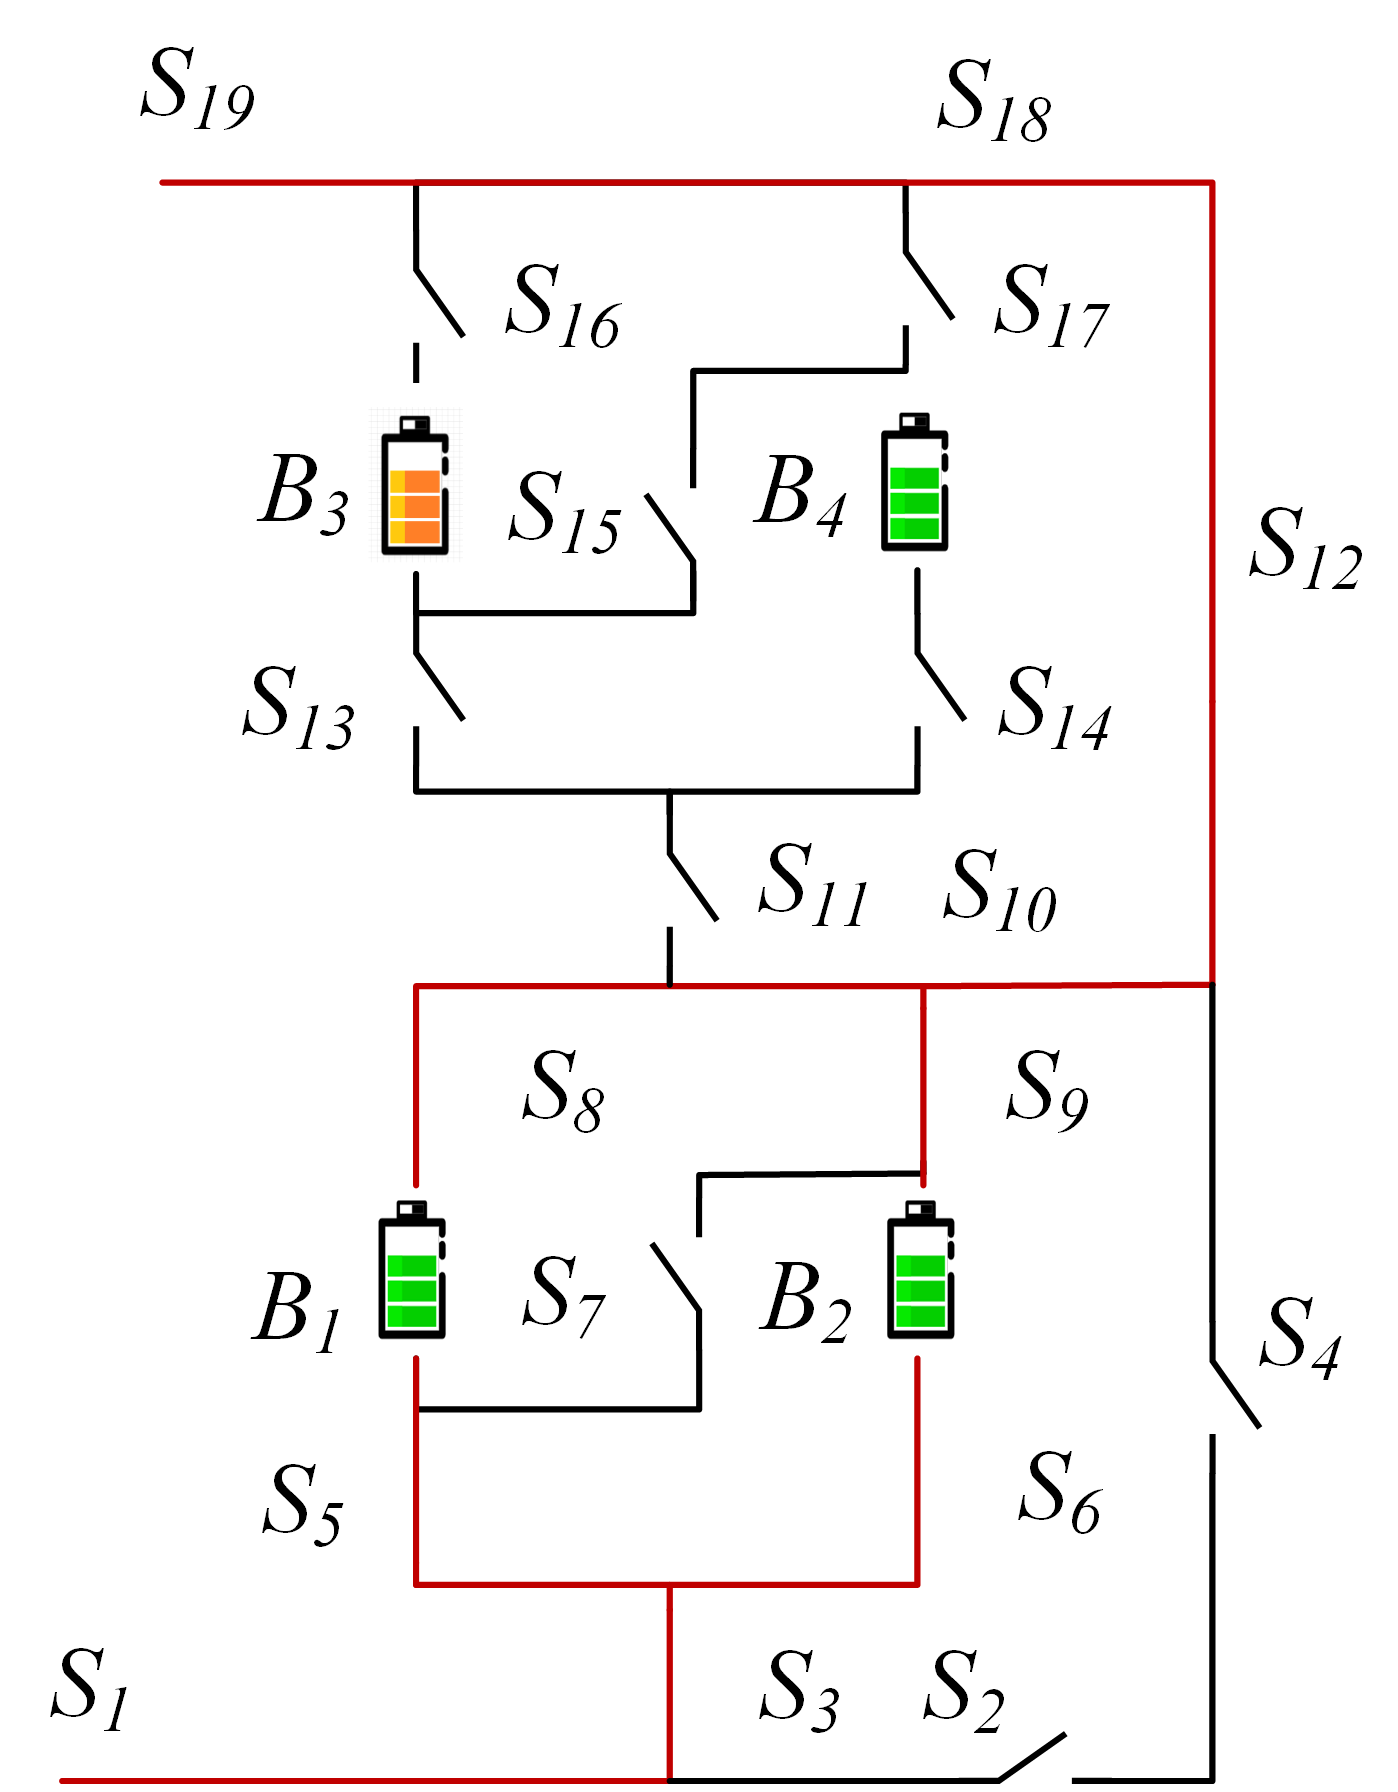
\includegraphics[width=\textwidth]{my-isolated-1.png}
          \caption{}
          \label{fig:my-isolated-1}
      \end{subfigure}
      \hspace{0.02\textwidth}
      \begin{subfigure}[b]{0.31\textwidth}
          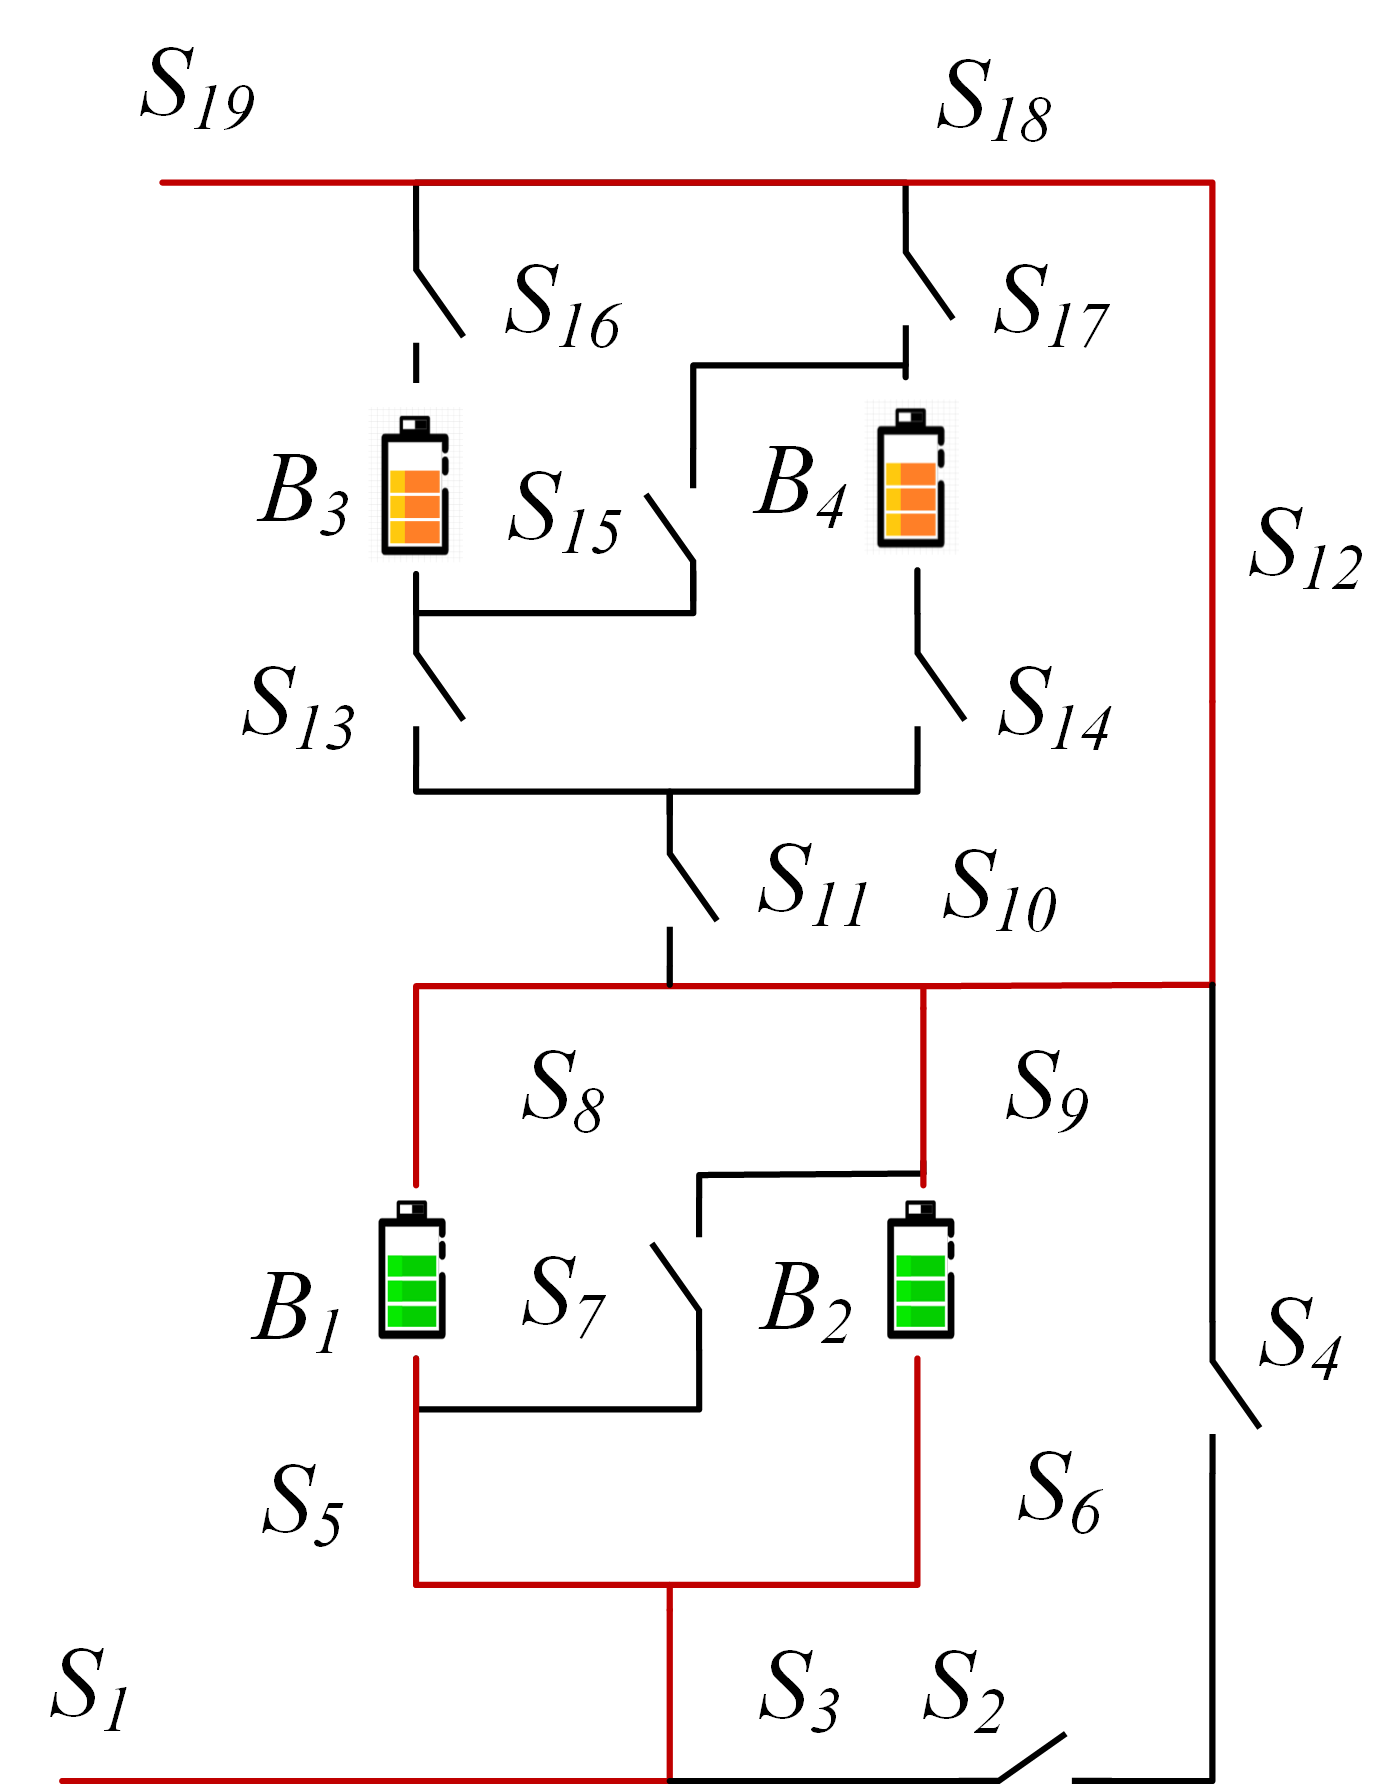
\includegraphics[width=\textwidth]{my-isolated-2b.png}
          \caption{}
          \label{fig:my-isolated-2b}
      \end{subfigure}
      \\
      \begin{subfigure}[b]{0.31\textwidth}
          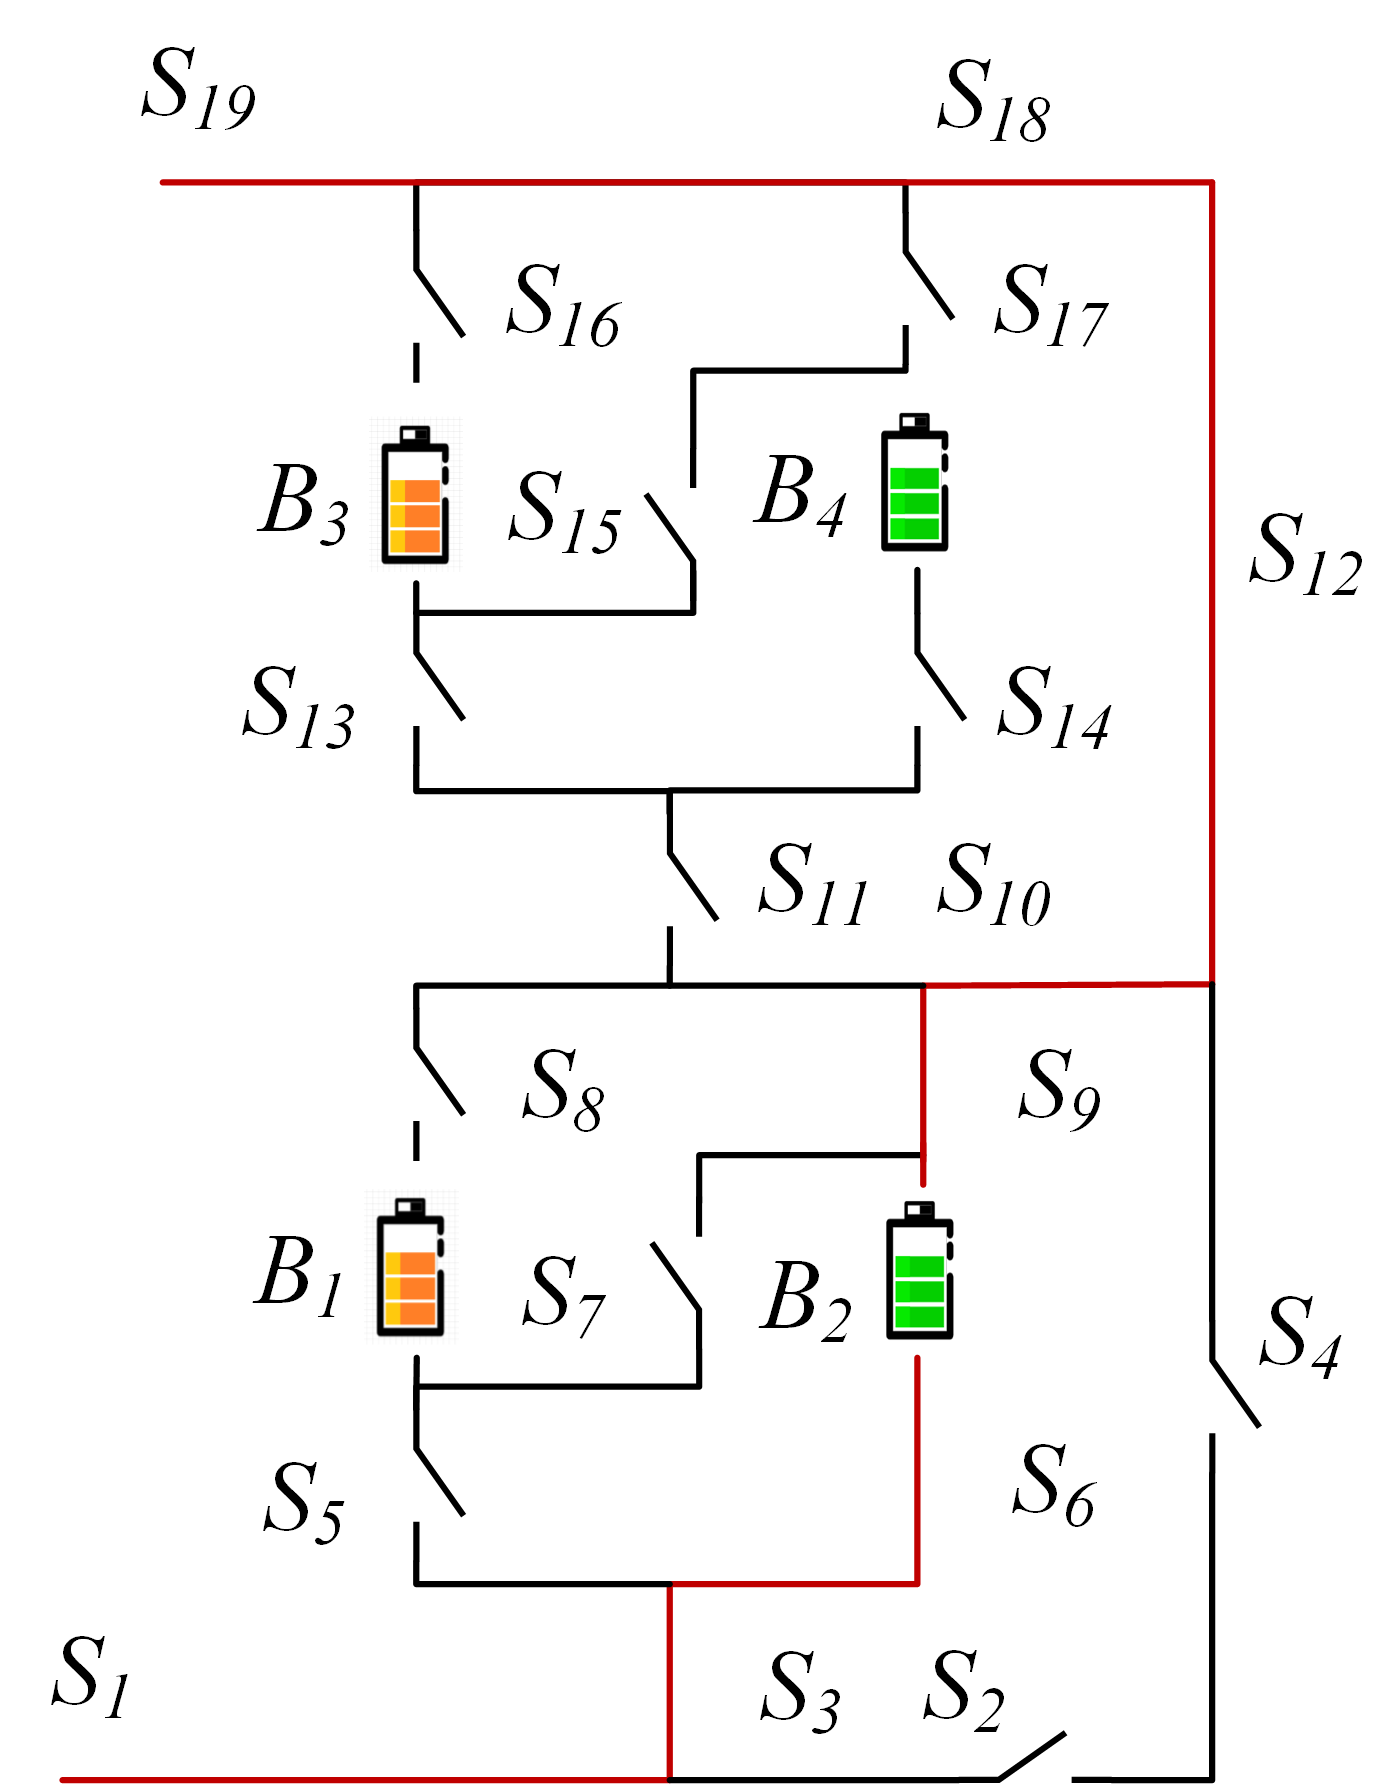
\includegraphics[width=\textwidth]{my-isolated-2w.png}
          \caption{}
          \label{fig:my-isolated-2w}
      \end{subfigure}
      \hspace{0.02\textwidth}
      \begin{subfigure}[b]{0.31\textwidth}
          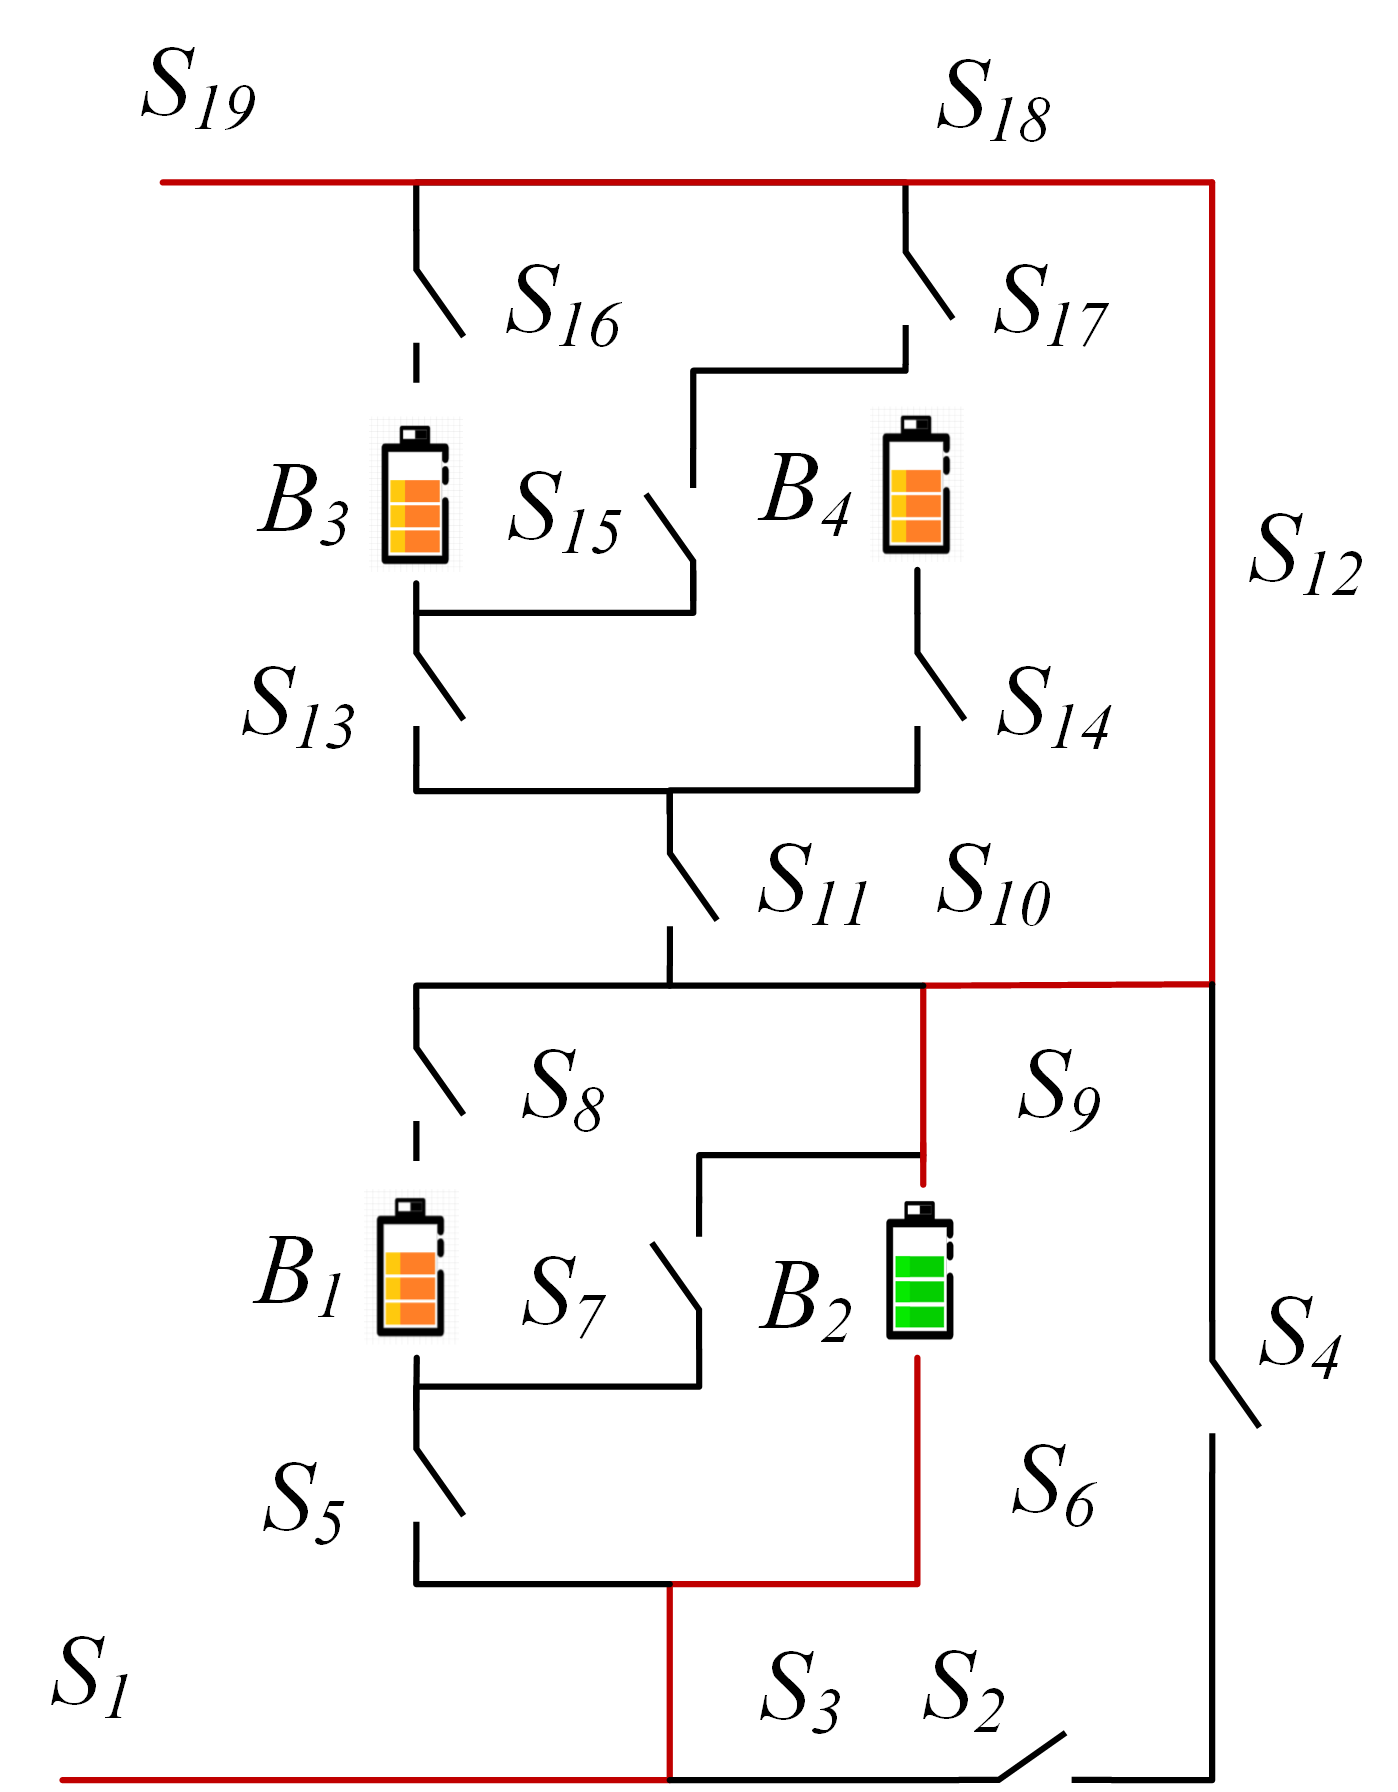
\includegraphics[width=\textwidth]{my-isolated-3.png}
          \caption{}
          \label{fig:my-isolated-3}
      \end{subfigure}
      \caption{
          \DIFdelbeginFL \DIFdelFL{The circuit }\DIFdelendFL \DIFaddbeginFL \DIFaddFL{Circuit }\DIFaddendFL states of MACs when isolating (a) one, (b) two (best case), (c) two (worst case)\DIFaddbeginFL \DIFaddFL{, }\DIFaddendFL and (d) three batteries for the structure in \DIFdelbeginFL \DIFdelFL{Figure }\DIFdelendFL \DIFaddbeginFL \DIFaddFL{Fig. }\DIFaddendFL \ref{fig:study-stru-my}.
          }
  \end{figure}

\subsection{Discussion}

\DIFdelbegin %DIFDELCMD < \replaced{As shown in Figure \ref{fig:all-results-my} and Table \ref{tab:study-results-my}}{In this subsection, we firstly discuss the correctness of the results presented in Figure \ref{fig:all-results-my} and Table \ref{tab:study-results-my}}%%%
\DIFdel{. }\DIFdelend \DIFaddbegin \DIFadd{Consider first the results shown in Fig. \ref{fig:all-results-my} and Table \ref{tab:study-results-my}.
}\DIFaddend When $B_1$ and $B_2$ or $B_3$ and $B_4$ are connected in parallel, the RBS \DIFdelbegin \DIFdel{can output }\DIFdelend \DIFaddbegin \DIFadd{outputs }\DIFaddend the maximum current, which is $\eta=2$ \DIFdelbegin \DIFdel{, }\DIFdelend \DIFaddbegin \DIFadd{(}\DIFaddend i.e., twice the current output of a single battery in \DIFdelbegin \DIFdel{RBS}\DIFdelend \DIFaddbegin \DIFadd{the RBS)}\DIFaddend . 
Adding more batteries to the main circuit \DIFdelbegin \DIFdel{can only form }\DIFdelend \DIFaddbegin \DIFadd{only forms }\DIFaddend a series structure and \DIFdelbegin \DIFdel{will }\DIFdelend \DIFaddbegin \DIFadd{does }\DIFaddend not improve the MAC. 
Therefore, the \DIFdelbegin \DIFdel{switches state }\DIFdelend \DIFaddbegin \DIFadd{state of the switches }\DIFaddend given in Table \ref{tab:study-results-my} \DIFdelbegin \DIFdel{can make }\DIFdelend \DIFaddbegin \DIFadd{maximizes }\DIFaddend the RBS output current\DIFdelbegin \DIFdel{reach the maximum.
}%DIFDELCMD < \added{The results of MAC obtained by brute force algorithm method is identical to the one by the greedy algorithm.}
%DIFDELCMD < %%%
\DIFdelend \DIFaddbegin \DIFadd{.
The MAC obtained by the brute-force algorithm is identical to the one obtained by the greedy algorithm.
}\DIFaddend 



\DIFdelbegin %DIFDELCMD < \added{
%DIFDELCMD < From the literature research we have conducted, no formal report on the algorithm for MAC in RBS has been found yet.
%DIFDELCMD < The brute force algorithm, which goes through all possible switch states, is the most straightforward way to solve the MAC problem and is used as a benchmark for the proposed greedy algorithm.
%DIFDELCMD < Assuming that a RBS has $N_b$ batteries and $N_s$ switches, and the corresponding directed graph has $N$ nodes, it requires $2^{N_s}$ iterations to traverse all reconfigured structures.
%DIFDELCMD < The calculation for each reconfigured structure by Equations \ref{eq:I_o}-\ref{eq:eta} requires matrix inversion and matrix multiplication, with a time complexity of $O(N^3+2N^2N_b+N^2N_s+NN^2_b)$.
%DIFDELCMD < Therefore, the time complexity of the brute force algorithm is $O(2^{N_s}(N^3+2N^2N_b+N^2N_s+NN^2_b))$.
%DIFDELCMD < The greedy algorithm proposed in this paper requires find the $SP$ for each battery, which requires $N_b$ iterations.
%DIFDELCMD < Each $SP$ can be obtained by couple Dijkstra algorithms.
%DIFDELCMD < Therefore, the total time complexity of calculating all $SP$s is $O(2N_b(N_b+2N_s)\log N)$.
%DIFDELCMD < According to the Appendix \ref{alg:greedy}, the RBS can reconfigure $C^{N_{set}}_{N_b}$ structures by selecting $N_{set}$ batteries from $N_b$ batteries, which is $\sum^{N_b}_{N_{set}=1}C^{N_{set}}_{N_b}/N_b \approx 2^{N_b}/N_b$ on average.
%DIFDELCMD < Hence, with bisection method, the time complexity of the greedy algorithm is $O(2^{N_b}/N_b(N^3+2N^2N_b+N^2N_s+NN^2_b)\log N_b+2N_b(N_b+2N_s)\log N)$, i.e., $O(2^{N_b}/N_b(N^3+2N^2N_b+N^2N_s+NN^2_b)\log N_b)$.
%DIFDELCMD < Based on currently proposed RBS structures\cite{ciNovelDesignAdaptive2007,alahmadBatterySwitchArray2008,kimDependableEfficientScalable2010b,kimBalancedReconfigurationStorage2011a,taesickimSeriesconnectedSelfreconfigurableMulticell2012a,6843711}, the number of batteries $N_b$, switches $N_s$, and nodes $N$ have the following quantitative relationships: $N_s \approx (3\sim 5)N_b$, $N \approx N_s$. 
%DIFDELCMD < After simplifying, the time complexity of the greedy algorithm is $O(2^{N_b}N_s^2\log N_b)$, while it is $O(2^{N_s}N_s^3)$ for brute force algorithm.
%DIFDELCMD < Therefore, it is reasonable to believe that as the size of the RBS increases, especially the number of the switches, the greedy algorithm will have an advantage over the algorithm that goes through all reconfigured structures.
%DIFDELCMD < This can be confirmed from the number of structures required for MAC determination in the previous subsection. 
%DIFDELCMD < Compared to the brute force algorithm, the efficiency of the method based on the greedy algorithm has been improved by 3000 to 75000 times, which is theoretically $N_s 2^{N_s - N_b} \log N_b$ times according to the above time complexity analysis.
%DIFDELCMD < Among the three RBS structures, the highest is the RBS structure with 19 switches (Figure \ref{fig:study-stru-my}).
%DIFDELCMD < This benefit from two key points:
%DIFDELCMD < (1) The $SP$s guide the RBS to reconfigure reasonable structures, rather than blindly going through all possible structures. This reduces the factor in complexity from $2^{N_s}$ to $2^{N_b}$, which is the main reason for the improvement in efficiency;
%DIFDELCMD < (2) The bisection method further accelerates this process.
%DIFDELCMD < However, the greedy algorithm proposed in this paper still contains exponential terms in the time complexity, which means it may not be able to handle extremely large-scale RBS structures.
%DIFDELCMD < }
%DIFDELCMD < %%%
\DIFdelend \DIFaddbegin \DIFadd{The literature contains no report on an algorithm for calculating the MAC of an RBS.
The brute-force algorithm, which goes through all possible switch states, is the most straightforward way to determine the MAC and is used as a benchmark for the proposed greedy algorithm.
If an RBS has $N_b$ batteries and $N_s$ switches and the corresponding directed graph has $N$ nodes,  $2^{N_s}$ iterations are required to traverse all reconfigured structures.
Calculating each reconfigured structure using Eqs. (\ref{eq:I_o})--(\ref{eq:eta}) requires matrix inversion and matrix multiplication, which has a time complexity of $O(N^3+2N^2N_b+N^2N_s+NN^2_b)$.
Therefore, the time complexity of the brute-force algorithm is $O\bm(2^{N_s}(N^3+2N^2N_b+N^2N_s+NN^2_b)\bm)$.
The greedy algorithm proposed in this paper requires  that $SP$ be found for each battery, which requires $N_b$ iterations.
Each $SP$ can be obtained by several applications of Dijkstra's algorithms.
Therefore, the total time complexity for calculating all $SP$s is $O\bm(2N_b(N_b+2N_s)\log_{10} N\bm)$.
According to  Appendix \ref{alg:greedy}, the RBS can reconfigure $C^{N_{\text{set}}}_{N_b}$ structures by selecting $N_{\text{set}}$ batteries from $N_b$ batteries, which gives $\sum^{N_b}_{N_{\text{set}}=1}C^{N_{\text{set}}}_{N_b}/N_b \approx 2^{N_b}/N_b$ on average.
Thus, with the bisection method, the time complexity of the greedy algorithm is $O\bm(2^{N_b}/N_b(N^3+2N^2N_b+N^2N_s+NN^2_b)\log_{10} N_b+2N_b(N_b+2N_s)\log_{10} N\bm)$ }[\DIFadd{i.e., $O\bm(2^{N_b}/N_b(N^3+2N^2N_b+N^2N_s+NN^2_b)\log_{10} N_b\bm)$}]\DIFadd{.
Based on currently proposed RBS structures \mbox{%DIFAUXCMD
\cite{ciNovelDesignAdaptive2007,alahmadBatterySwitchArray2008,kimDependableEfficientScalable2010b,kimBalancedReconfigurationStorage2011a,taesickimSeriesconnectedSelfreconfigurableMulticell2012a,6843711}}\hskip0pt%DIFAUXCMD
, the number $N_b$ of batteries, $N_s$ of switches, and $N$ of nodes are quantitatively related as follows: $N_s \approx (3\text{--} 5)N_b$, $N \approx N_s$. 
After simplifying, the time complexity of the greedy algorithm is $O(2^{N_b}N_s^2\log N_b)$, while it is $O(2^{N_s}N_s^3)$ for brute force algorithm.
Therefore, as the RBS grows, especially in the number of switches, the greedy algorithm gains an advantage over the brute-force algorithm.
}\DIFaddend 

\DIFdelbegin \DIFdel{It is important to note that }%DIFDELCMD < \deleted{when solving for MAC,} %%%
\DIFdelend \DIFaddbegin \DIFadd{This is confirmed by the number of structures required to determine the MAC in the previous section. 
Compared with the brute-force algorithm, the method based on the greedy algorithm is 3000 to 75\,000 times more efficient, which is theoretically $N_s 2^{N_s - N_b} \log_{10} N_b$ times according to the above time-complexity analysis.
Of the three RBS structures, the largest is the RBS structure with 19 switches (Fig. \ref{fig:study-stru-my}).
This benefits from two key points:
}\begin{enumerate}
\item[\DIFadd{(1)}] \DIFadd{The $SP$s guide the RBS to reconfigure reasonable structures rather than blindly going through all possible structures. This reduces the complexity from $2^{N_s}$ to $2^{N_b}$, which is the main reason for the improvement in efficiency.
}\item[\DIFadd{(2)}] \DIFadd{The bisection method further accelerates this process.
However, the greedy algorithm proposed in this paper still contains exponential terms in the time complexity, which means it may not be able to handle extremely large RBS structures. 
}\end{enumerate}



\DIFadd{Note that }\DIFaddend $\eta$ is used as the objective function instead of $I_o$ \DIFdelbegin %DIFDELCMD < \added{in solving MAC}%%%
\DIFdelend \DIFaddbegin \DIFadd{in solving for the MAC}\DIFaddend . 
This choice makes the \DIFdelbegin \DIFdel{result of }\DIFdelend \DIFaddbegin \DIFadd{resulting }\DIFaddend MAC more reasonable. 
As shown in Table \ref{tab:study-results-my}, $I_o$ and $\bm{I}_b$ are functions of $R_o$, $u_b$, and $r_b$. 
\DIFdelbegin %DIFDELCMD < \replaced{However, when}{If} %%%
\DIFdelend \DIFaddbegin \DIFadd{However, when }\DIFaddend $I_o$ \DIFdelbegin %DIFDELCMD < \replaced{was}{were} %%%
\DIFdelend \DIFaddbegin \DIFadd{is }\DIFaddend used as the objective function, even for the same RBS structure, the MAC \DIFdelbegin %DIFDELCMD < \replaced{solution}{result} %%%
\DIFdel{and corresponding switches state }\DIFdelend \DIFaddbegin \DIFadd{solution and corresponding switch states }\DIFaddend could change due to different external electrical appliances.
\DIFdelbegin \DIFdel{It }\DIFdelend \DIFaddbegin \DIFadd{This }\DIFaddend would increase the difficulty and uncertainty \DIFdelbegin \DIFdel{in RBS structuredesign. 
}%DIFDELCMD < \replaced{In order to eliminate the influences of such a problem, $\eta$, which is the ratio of $I_o$ and $\max\bm{I}_b$, is adopted as the objective function in our research.}{In contrast, by using $\eta$ as the objective function, which is defined as the ratio of $I_o$ and $\max\bm{I}_b$, the influence of these factors on the results can be eliminated.}
%DIFDELCMD < %%%
\DIFdelend \DIFaddbegin \DIFadd{of designing the RBS structure. 
To eliminate this problem, the ratio $\eta=I_o/\max\bm{I}_b$ is adopted as the objective function in our research.
Recall that }\DIFaddend $\eta$ \DIFdelbegin \DIFdel{solely reflects the maximum output current capability }\DIFdelend \DIFaddbegin \DIFadd{reflects only the MAC }\DIFaddend of the RBS structure. 
Assuming that the \DIFdelbegin \DIFdel{maximum allowed current }\DIFdelend \DIFaddbegin \DIFadd{MAC }\DIFaddend of batteries in the RBS is $I_m$, the maximum output current of the RBS structure can be calculated as $\eta I_m$ by determining the \DIFdelbegin \DIFdel{$\eta$ of }\DIFdelend \DIFaddbegin \DIFadd{value of $\eta$ for }\DIFaddend the structure. 
\DIFdelbegin %DIFDELCMD < \deleted{Therefore, compared to $I_o$, $\eta$ is more suitable for structure design.}
%DIFDELCMD < %%%
\DIFdelend 


The method proposed in this paper \DIFdelbegin \DIFdel{is significant for }\DIFdelend \DIFaddbegin \DIFadd{facilitates }\DIFaddend the design of \DIFdelbegin %DIFDELCMD < \deleted{next-generation} %%%
\DIFdelend RBSs in the following \DIFdelbegin \DIFdel{aspects.
Most of the }\DIFdelend \DIFaddbegin \DIFadd{ways:
Most }\DIFaddend currently proposed RBS structures \cite{ciNovelDesignAdaptive2007,alahmadBatterySwitchArray2008,kimDependableEfficientScalable2010b,kimBalancedReconfigurationStorage2011a,taesickimSeriesconnectedSelfreconfigurableMulticell2012a,6843711} \DIFdelbegin \DIFdel{exhibit }\DIFdelend \DIFaddbegin \DIFadd{have }\DIFaddend simple topological characteristics, \DIFdelbegin \DIFdel{and the calculation of }\DIFdelend \DIFaddbegin \DIFadd{so calculating the }\DIFaddend MACs is relatively straightforward, even intuitive.
However, these simple structures do not always fully satisfy the requirements of complex applications, such as dynamically adapting the circuit to variable and random operating conditions \DIFdelbegin \DIFdel{, and }\DIFdelend \DIFaddbegin \DIFadd{or }\DIFaddend actively equalizing differences \DIFdelbegin \DIFdel{among the }\DIFdelend \DIFaddbegin \DIFadd{between }\DIFaddend batteries in the RBS.
Moreover, \DIFdelbegin %DIFDELCMD < \replaced{isolation of}{isolating} %%%
\DIFdelend \DIFaddbegin \DIFadd{isolating }\DIFaddend the batteries disrupts the original regularity and symmetry of the topology, which complicates the otherwise simple structure, and the maximum output current of the system becomes more challenging to obtain.
\DIFdelbegin %DIFDELCMD < \replaced{On the contrary}{Owing to the advantages of pervasiveness and automation}%%%
\DIFdelend \DIFaddbegin \DIFadd{In contrast}\DIFaddend , the proposed method \DIFdelbegin \DIFdel{can be employed to calculate }\DIFdelend \DIFaddbegin \DIFadd{calculates }\DIFaddend the MAC of arbitrary RBS structures, \DIFdelbegin %DIFDELCMD < \replaced{especially for these above complex and flexible RBS structures}{which helps to address the aforementioned issues and paves the way for more complex and flexible RBS structure design}%%%
\DIFdelend \DIFaddbegin \DIFadd{notably the complex and flexible RBS structures}\DIFaddend .


To illustrate this point, the MACs of \DIFdelbegin %DIFDELCMD < \deleted{the} %%%
\DIFdelend three RBS structures mentioned above are calculated after \DIFdelbegin %DIFDELCMD < \replaced{one and more}{the} %%%
\DIFdel{batteriesare isolated}\DIFdelend \DIFaddbegin \DIFadd{isolating one or more of the batteries}\DIFaddend , as shown in Table \ref{tab:isolated_mac}. 
Specifically, for the structure presented in \DIFdelbegin \DIFdel{Figure }\DIFdelend \DIFaddbegin \DIFadd{Fig. }\DIFaddend \ref{fig:study-stru-my}, the corresponding circuit states \DIFdelbegin \DIFdel{of MACs }%DIFDELCMD < \replaced{of}{when} %%%
\DIFdel{isolating }%DIFDELCMD < \replaced{one to three}{different numbers of} %%%
\DIFdelend \DIFaddbegin \DIFadd{for the MACs when isolating one to three }\DIFaddend batteries are depicted in \DIFdelbegin \DIFdel{Figures \ref{fig:my-isolated-1}-}\DIFdelend \DIFaddbegin \DIFadd{Figs. \ref{fig:my-isolated-1}--}\DIFaddend \ref{fig:my-isolated-3}. 
This structure has two cases \DIFdelbegin \DIFdel{of isolating two batteries }\DIFdelend \DIFaddbegin \DIFadd{in which two batteries are isolated}\DIFaddend : 
one is to isolate two batteries within the same substructure (\DIFdelbegin \DIFdel{Figure }\DIFdelend \DIFaddbegin \DIFadd{Fig. }\DIFaddend \ref{fig:my-isolated-2b}), in which case $\eta=2$; the other is to isolate one battery in each of the two substructures (\DIFdelbegin \DIFdel{Figure }\DIFdelend \DIFaddbegin \DIFadd{Fig. }\DIFaddend \ref{fig:my-isolated-2w}), in which case $\eta=1$. 
\DIFdelbegin \DIFdel{From the results }%DIFDELCMD < \added{shown in Figure \ref{fig:my-isolated-1}-\ref{fig:my-isolated-3}}%%%
\DIFdel{, it can be observed }\DIFdelend \DIFaddbegin \DIFadd{The results in Figs. \ref{fig:my-isolated-1}--\ref{fig:my-isolated-3} show }\DIFaddend that the proposed method provides reasonable outcomes for isolating \DIFdelbegin \DIFdel{batteries with any number and }\DIFdelend \DIFaddbegin \DIFadd{any number of batteries in any }\DIFaddend position.


Furthermore, the \DIFdelbegin %DIFDELCMD < \deleted{performance of} %%%
\DIFdelend output current for the three \DIFdelbegin \DIFdel{RBS }%DIFDELCMD < \replaced{with isolated}{when isolating} %%%
\DIFdelend \DIFaddbegin \DIFadd{RBSs with isolated }\DIFaddend batteries is also shown in Table \ref{tab:isolated_mac}. 
For the structure proposed by Lawson et al., the MAC \DIFdelbegin %DIFDELCMD < \replaced{is independent on the number of isolated batteries}{remains the same as that without isolated battery cells, i.e., $\eta=1$, when the number of isolated battery cells increases, until all the cells in the RBS are isolated}%%%
\DIFdel{.
}%DIFDELCMD < \added{However,} \replaced{f}{F}%%%
\DIFdel{or }\DIFdelend \DIFaddbegin \DIFadd{is independent of the number of isolated batteries.
However, for }\DIFaddend Visairo's structure, the MAC decreases \DIFdelbegin %DIFDELCMD < \replaced{with the increasing number of isolated batteries}{as the number of isolated battery cells increases, until $\eta=0$}%%%
\DIFdel{. 
}%DIFDELCMD < \replaced{Nevertherless}{In contrast}%%%
\DIFdelend \DIFaddbegin \DIFadd{upon increasing the number of isolated batteries. 
Nevertheless}\DIFaddend , the MAC of the structure proposed in this work \DIFdelbegin \DIFdel{is positioned between }%DIFDELCMD < \replaced{these above}{the} %%%
\DIFdelend \DIFaddbegin \DIFadd{falls between the MACs of these }\DIFaddend two structures. 
This \DIFaddbegin \DIFadd{result }\DIFaddend indicates that the structure proposed in this paper \DIFdelbegin \DIFdel{, compared to Lawson's structure, }\DIFdelend has a larger MAC \DIFdelbegin \DIFdel{under }\DIFdelend \DIFaddbegin \DIFadd{than Lawson's for }\DIFaddend the same number of batteries \DIFdelbegin \DIFdel{, }%DIFDELCMD < \replaced{and exhibits}{which means} %%%
\DIFdel{a wider output current regulation range. 
}%DIFDELCMD < \deleted{On the other hand, by simply changing the states of $S_2$, $S_4$, $S_{11}$, and $S_{12}$ in the conversion structure, this structure can address the majority of battery isolation scenarios, whereas Visairo's structure requires specific battery targeting and switch control.}
%DIFDELCMD < \deleted{In summary, the structure proposed in this paper has the advantages of both Lawson's and Visairo's structures.}
%DIFDELCMD < %%%
\DIFdelend \DIFaddbegin \DIFadd{and has a wider range of regulation of the output current. 
}\DIFaddend 

\section{Conclusion}

This paper proposes a pervasive and \DIFdelbegin \DIFdel{automatical method for computing }\DIFdelend \DIFaddbegin \DIFadd{automated method to efficiently compute }\DIFaddend the MAC of \DIFdelbegin %DIFDELCMD < \replaced{a}{the} %%%
\DIFdel{given RBS}%DIFDELCMD < \added{efficiently}%%%
\DIFdel{.
}%DIFDELCMD < \added{
%DIFDELCMD < The method is implemented by a greedy algorithm combined with a directed graph model which considers the voltage, internal resistance, and maximum allowable current of the batteries, as well as the external load.
%DIFDELCMD < The main advantage of this method is its ability to calculate the MAC of RBSs with arbitrary structures.
%DIFDELCMD < Even in the scenarios with random isolated batteries, the method remains effective.
%DIFDELCMD < Compared with the brute force algorithm, the proposed method has higher computational efficiency under the same calculation results.
%DIFDELCMD < This is achieved by two key points when constructing the greedy algorithm: 
%DIFDELCMD < (1) Calculate the shortest path of each battery by Dijkstra algorithm to obtain the $SP$ of each battery; 
%DIFDELCMD < (2) determine the maximum number of available batteries by bisection method to reduce the computational complexity.
%DIFDELCMD < This method helps to fully tap the current output potential of the RBS, guide the RBS structure design and optimization in the design stage, and assist in evaluating the current overload risk of the system in practical applications.
%DIFDELCMD < }
%DIFDELCMD < \deleted{The method is implemented by a greedy algorithm combined with a directed graph model , whose effectiveness is tested on a novel and complex RBS structure.
%DIFDELCMD < The method remains effective for the application scenario of RBS battery isolation and demonstrates that the novel structure has the advantage on flexible output current and convenient battery isolation.
%DIFDELCMD < Future research could focus on developing new indictors to evaluate the performance of the RBS with the currents and voltages obtained by the method, as well as modifying the equivalent model of the battery to allow for more accurate simulations of the RBS, including transient analysis.}
%DIFDELCMD < %%%
\DIFdelend \DIFaddbegin \DIFadd{a RBS.
The method is implemented by a greedy algorithm combined with a directed graph model that considers the voltage, internal resistance, and MAC of the batteries, as well as the external load.
The main advantage of this method is its ability to calculate the MAC of RBSs with arbitrary structures.
Even in scenarios with random isolated batteries, the proposed method remains effective.
The proposed method is more computationally efficient than the brute-force algorithm for the same calculation results, which is achieved by two key points when constructing the greedy algorithm: 
}\begin{enumerate}
\item[\DIFadd{(1)}] \DIFadd{Calculate the shortest path of each battery by using the Dijkstra algorithm to obtain the $SP$ for each battery. 
}\item[\DIFadd{(2)}] \DIFadd{Determine the maximum number of available batteries by bisection to reduce the computational complexity.
}\end{enumerate}
\DIFadd{This method helps to fully tap the current output potential of the RBS, guide the RBS structure design and optimization in the design stage, and assist in evaluating the current-overload risk of the system in practical applications.
}\DIFaddend 


\section{Appendix} 

\begin{algorithm}
    \caption{Get the max available currents of a certain RBS}\label{alg:greedy}
    \KwData{Directed graph model $G(V,E)$ of the RBS}
    \KwResult{$\max \eta$}
    \For{$i \in E_b$}{
        $P_i \leftarrow \{path| \text{starts at $v_1$ and ends at $v_n$} \}$\;
        $SP_i \leftarrow p_i \text{ which has the minimum}~\omega(p_i)~\text{among all}~p_i \in P_i. $
    }
    get $\bm{A}$ by Equation \ref{eq:A}\;
    \While{not yet determine $\max \eta$ }
    {
        \DIFdelbegin \DIFdel{$N_{set} \leftarrow$ }\DIFdelend \DIFaddbegin \DIFadd{$N_{\text{set}} \leftarrow$ }\DIFaddend number of setected $SP$s calculated by dichotomy\;
        $C_b    \leftarrow$ set of all combinations of \DIFdelbegin \DIFdel{$N_{set} $}\DIFdelend \DIFaddbegin \DIFadd{$N_{\text{set}} $}\DIFaddend ~batteries from $N_b$\;
        \DIFdelbegin %DIFDELCMD < \For{$c_b \in C_b$}{
%DIFDELCMD <             $\bm{x}_s \leftarrow \text{list of all switches' state: $x_s[j]=1$ if $ j \in \bigcup_{i\in c_b}SP_i $ else 0}$\;
%DIFDELCMD <             $\bm{X} \leftarrow diag[1,1,\cdots,1,\bm{x}_s] $\;
%DIFDELCMD <             get $\bm{Y}_n$ by Equation \ref{eq:Yn}\;
%DIFDELCMD <             \eIf{$\bm{Y}_n$ is invertible}{
%DIFDELCMD <               \added{pass}
%DIFDELCMD <             }{construct an effective solution}
%DIFDELCMD <             get $I_o$ by Equation \ref{eq:I_o}\;
%DIFDELCMD <             get $\bm{I}_b$ by Equation \ref{eq:I_b}\;
%DIFDELCMD <             \eIf{$\max(\bm{I}_b)\leq I_m$}{
%DIFDELCMD <                 $\eta \leftarrow I_o/\max(\bm{I}_b)$\;
%DIFDELCMD <             }{break}
%DIFDELCMD <         }
%DIFDELCMD <     %%%
\DIFdelend \DIFaddbegin \For{$c_b \in C_b$}{
            $\bm{x}_s \leftarrow \text{list of all switches' state: $x_s[j]=1$ if $ j \in \bigcup_{i\in c_b}SP_i $ else 0}$\;
            $\bm{X} \leftarrow diag[1,1,\cdots,1,\bm{x}_s] $\;
            get $\bm{Y}_n$ by Equation \ref{eq:Yn}\;
            \eIf{$\bm{Y}_n$ is invertible}{
              pass
            }{construct an effective solution}
            get $I_o$ by Equation \ref{eq:I_o}\;
            get $\bm{I}_b$ by Equation \ref{eq:I_b}\;
            \eIf{$\max(\bm{I}_b)\leq I_m$}{
                $\eta \leftarrow I_o/\max(\bm{I}_b)$\;
            }{break}
        }
    \DIFaddend }
\end{algorithm}
% \begin{figure}[htbp]
%     \centering
%     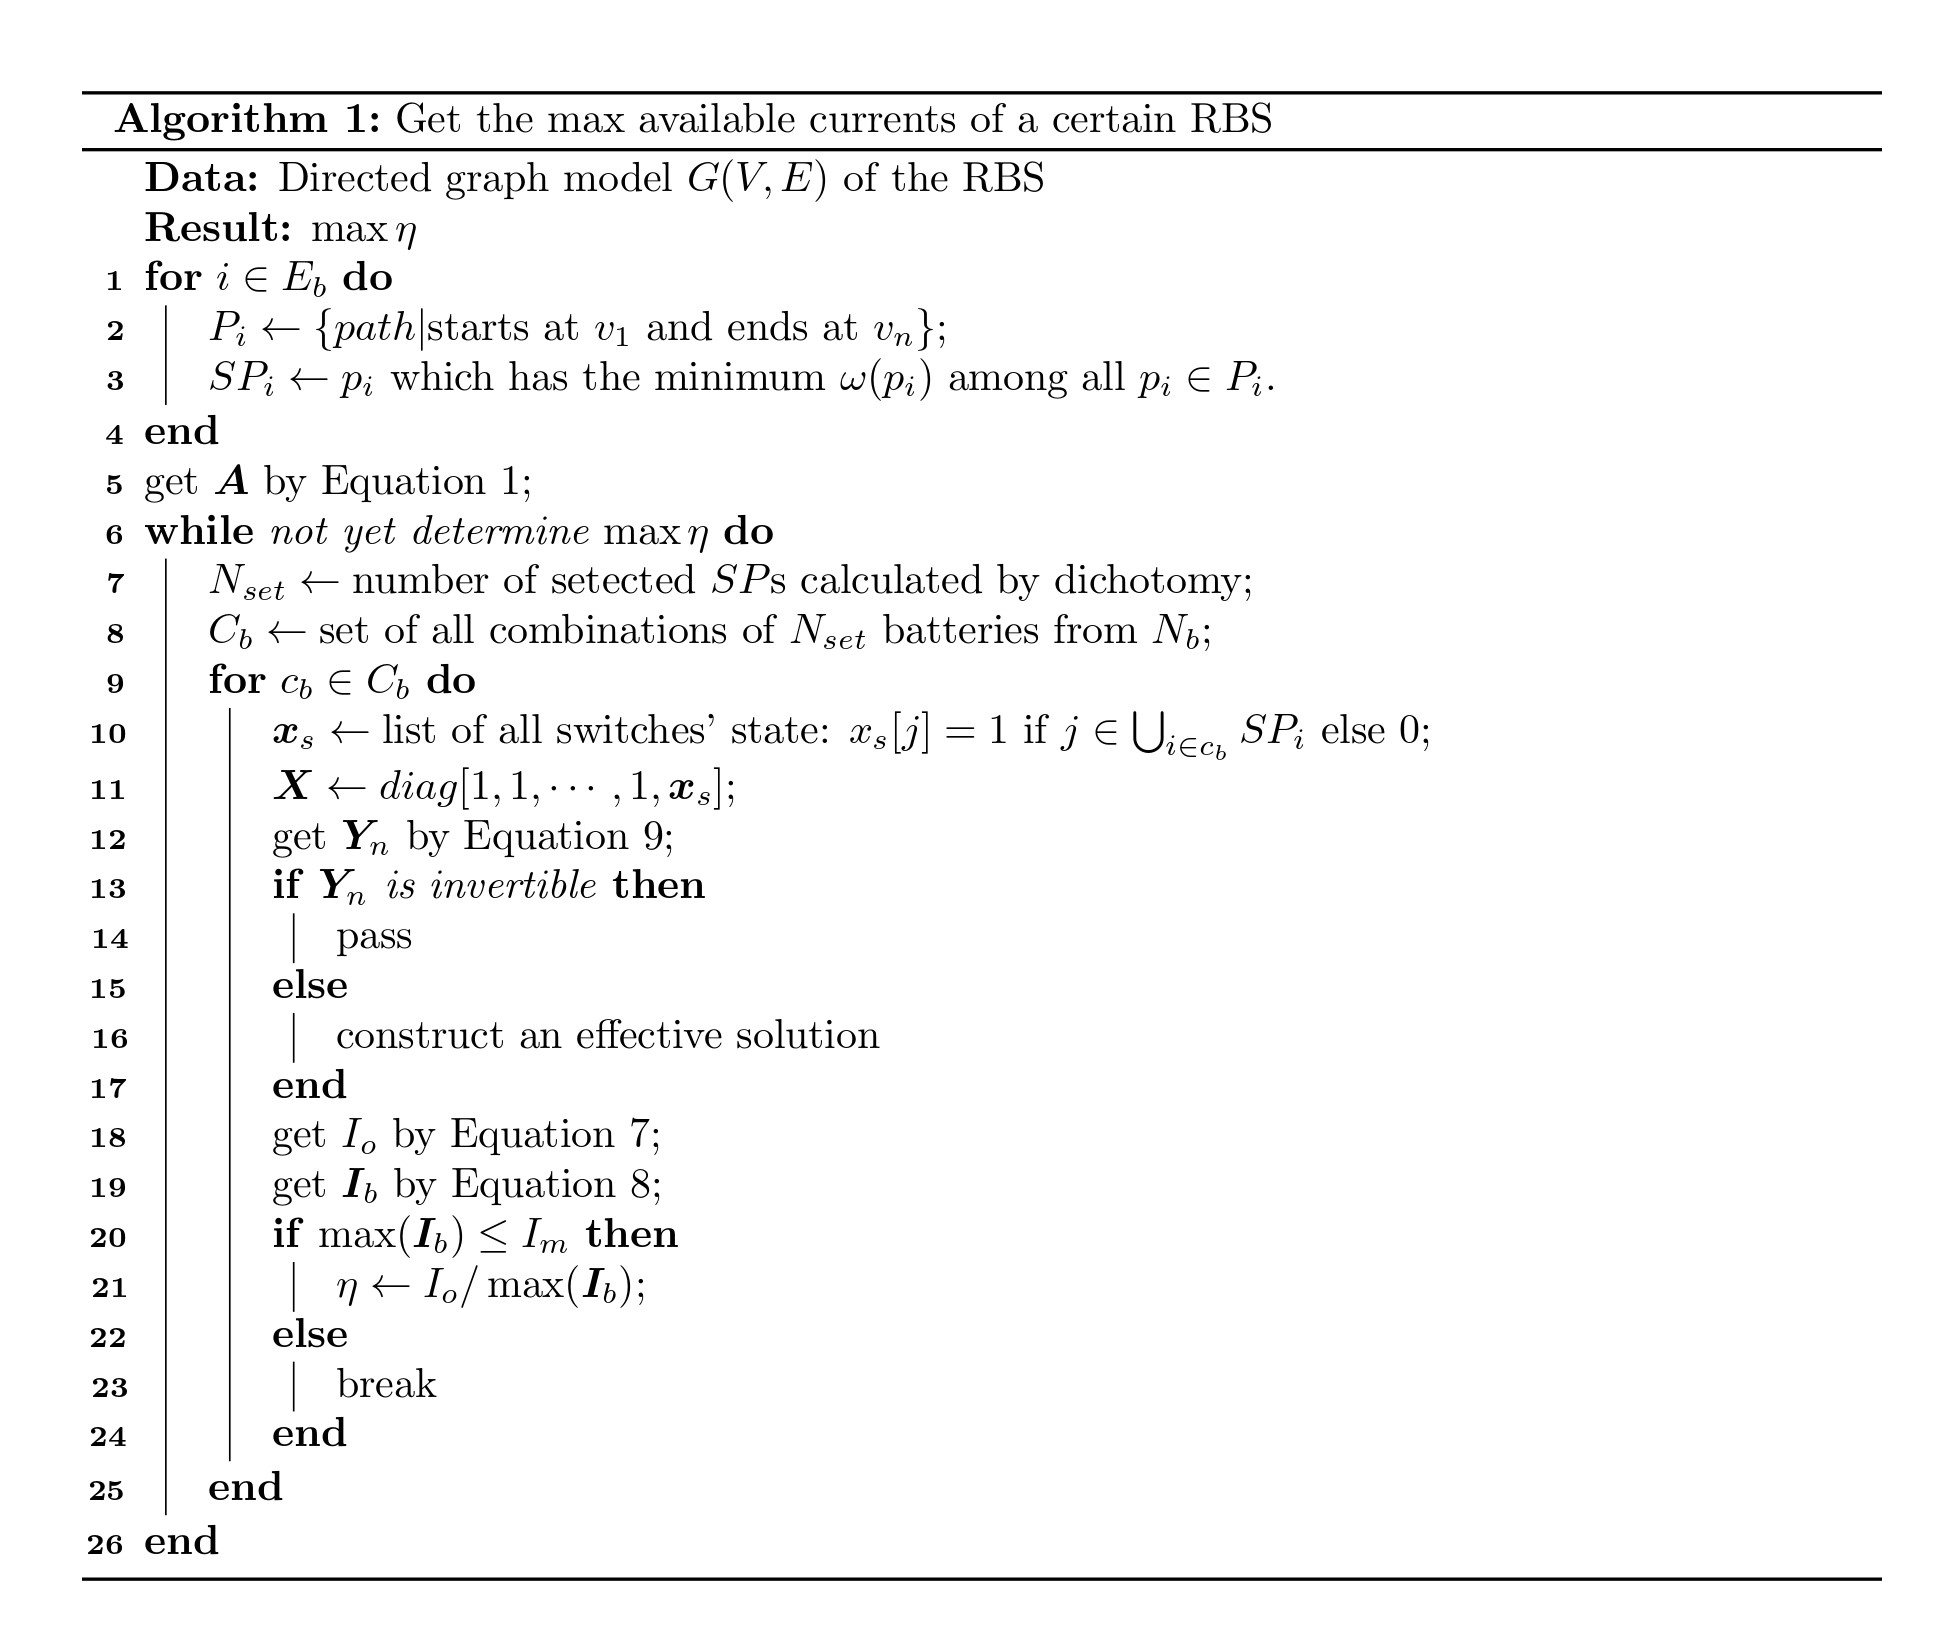
\includegraphics[width=\textwidth]{algorithm.jpg}
% \end{figure}


\section*{Acknowledgments}

\subsection*{Author Contributions} 

B. Xu conceived the main idea, formulated the overarching research goals and aims, designed the algorithm, and reviewed and revised the manuscript.
G. Hua developed and analyzed the model, implemented the code and supporting algorithms, and wrote the initial draft.
C. Qian provided critical review, commentary, and revisions.
Q. Xia contributed to shaping the research, analysis, and manuscript.
B. Sun conducted the research and investigation process.
Y. Ren secured the funding and supervised the project.
Z. Wang verified the results and provided necessary resources.

\subsection*{Funding}

This work was supported by the National Natural Science Foundation of China (NSFC, No.52075028).

\subsection*{Conflicts of Interest}

The authors declare that there is no conflict of interest regarding the publication of this article.

\subsection*{Data Availability}

This work does not require any data to be declared or publicly disclosed.

% \bibliographystyle{nejm}
% \bibliography{sst_main}

\printbibliography

\end{document}
